\documentclass{ufpatcc}

\include{include}
%% Packages used for the TCC

%\usepackage{booktabs}

%%%% Definitions and New commnads %%%%

\newcommand{\sen}{\operatorname{sen}}
\newcommand{\mbeq}{\overset{!}{=}}

\renewcommand\Re{\operatorname{Re}}
\renewcommand\Im{\operatorname{Im}}

%%%% New control sequences %%%%

\newcommand{\redeq}[1] {\textcolor{red}{#1}}
\newcommand{\blueeq}[1] {\textcolor{blue}{#1}}
\newcommand{\att}[1] {\textcolor{red}{#1}}
% Used Packages:
\usepackage{tikz}
\usepackage{float}
\usepackage{steinmetz}
\usetikzlibrary{arrows,shapes,shapes.multipart}
\usepackage[brazil]{babel}
\usepackage[T1]{fontenc}
\usepackage[utf8]{inputenc}
\usepackage{amsmath}
\usepackage{amsfonts}
%\usepackage{enumitem} % To adjust lists
\usepackage{verbatim} % Multi-line comments
\usepackage{mathabx} % Package that contains the circular convolution symbol
\usepackage{graphicx}
\usepackage{caption}
\usepackage{subcaption}
\usepackage{units}
\usepackage{adjustbox}
\usepackage{dirtytalk}
\usepackage{csquotes}
\usepackage{enumerate}
\usepackage{url} 
\usepackage[pdfusetitle]{hyperref}
\usepackage{breakurl}
\usepackage{array}  
\usepackage{eurosym}


\usepackage{siunitx} %símbolo OHM

%\usepackage[backend=bibtex8]{biblatex}
%\makeatletter
%\providecommand\@enumctr{}
%\makeatother

\ifpdf

\ifdefined\hyperref
\else
\usepackage[pdftex,colorlinks]{hyperref}
\fi

\hypersetup{%
pdftitle={Some title},
pdfauthor={Your name - LaPS - UFPA},
pdfkeywords={DSP,Signal},
pdfstartview={FitH}, %% <--
urlcolor=black,
%linkcolor=blue,
linkcolor=black,
%citecolor=red,
citecolor=black,
}

% Ensiar o Latex a separar silabas
\hyphenation{DMT En-ge-nhei-ro}


\hypersetup{%
	pdftitle={Trabalho de Conclusão de Curso},
	pdfauthor={Erick Modesto Campos},
	pdfkeywords={Tecnologia Assistiva, Acessibilidade},
	pdfstartview={FitH}, %% <--
	urlcolor=black,
	linkcolor=black,
	citecolor=black,
}

\graphicspath{{fig/}}
%Uma Proposta de Clique do \textit{Mouse} Baseado em Sopro
\ufpaTitulo{Uma Proposta de Acionador Externo de Baixo Custo Baseado em Sopro}

\ufpaAutor{Erick Modesto Campos}
\ufpaAno{2018}
\ufpaSegundoAutor{} % Segundo autor, se necessario
\ufpaOrientador{MSc. Cassio Trindade Batista}
\ufpaCoOrientador{Prof. Dr. Nelson Cruz Sampaio Neto}
\ufpaMembroBancaA{Prof. Dr. Filipe de Oliveira Saraiva}
\ufpaMembroBancaB{Prof. Dr. Marcos André Barros Galhardo}
\ufpaCoordenadorCurso{Prof. Dr. Marcos César da Rocha Seruffo}

\usepackage{titlesec}

\begin{document}

\ufpaPaginaDeRosto

\pagenumbering{roman}

\ufpaPagRostodo 

\ufpaPaginaDeAprovacao

%%%%%%%%%%%%%%%%%%%%
%   Oferecimento   %
%%%%%%%%%%%%%%%%%%%%

\begin{ufpaOferecimento}
	\index{Oferecimento@Oferecimento}%
	\addcontentsline{toc}{chapter}{Dedicatória} 
    “Dedico esse trabalho à minha família e amigos”

\end{ufpaOferecimento}

%%%%%%%%%%%%%%%%%%%%
%  Agradecimento   %
%%%%%%%%%%%%%%%%%%%%

\begin{ufpaAgradecimentos}
	\chapter*{Agradecimentos}
	\index{Agradecimentos@Agradecimentos}% 
	\addcontentsline{toc}{chapter}{Agradecimentos} 
    %ok
	Primeiramente, agradeço à minha família, por toda ajuda e apoio que foram de
fundamental importância tanto para a minha formação pessoal quanto profissional.
Em especial, à minha mãe Cláudia Modesto e meu padrasto Edevaldo Trindade, por
sempre confiarem e me apoiarem em todas as minhas decisões. Agradeço também aos
meus avós e a todos os meus tios e primos, que sempre estiveram, direta ou
indiretamente, ao meu lado. Amo vocês. Um dia espero retribuir tudo o que vocês
já fizeram por mim.

Agradeço em especial à Suzane Santos, pelo carinho, companhia, ajuda e
conselhos. Sem dúvidas, você foi uma das pessoas mais importantes para mim nos
últimos quatro anos. Não se esqueça que apenas vou atravessar a ponte do básico 
e que sempre vou estar ao seu lado. Amo você, mulher.  

Aos meus orientadores Cassio Batista e Nelson Neto, pela confiança no trabalho
que venho desenvolvendo há dois anos; pela paciência e também pelos ``puxões de
orelha'' que me ajudaram a crescer academicamente. 

Agradeço também aos meus amigos Daniel Breno, Israel Lucas, Rodrigo Lima pelas
inúmeras ajudas ao longo do curso. Certamente não poderia deixar de agradecer à
todos os demais colegas do curso de Engenharia da Computação e Engenharia de
Telecomunicações, os quais não conseguiria listar e, por isso, não ouso citar
nomes.

Aos professores da Engcomp/FCT, sem os quais não teria a disciplina e o
conhecimento necessários para o desenvolvimento deste trabalho.

Por fim, Agradeço aos voluntários que aceitaram participar dos testes, sem as quais
os resultados e conclusões deste trabalho não teriam sido possíveis.

	
	
\end{ufpaAgradecimentos}

%%%%%%%%%%%%%%%%%%%%
%      Epigrafe     %
%%%%%%%%%%%%%%%%%%%%

\begin{ufpaEpigrafe}
    ``Todas as vitórias ocultam uma abdicação''
    \begin{flushright}Simone De Beauvoir\end{flushright}
\end{ufpaEpigrafe}

%%%%%%%%%%%%%%%%%%%%
%      Resumo      %
%%%%%%%%%%%%%%%%%%%%


%sumário
\tableofcontents
\clearpage

%\begin{ufpaResumo}
%
%    Resumo do TCC
%
%\end{ufpaResumo}
%
%\begin{abstract}
%
%    Abstract written in english
%
%\end{abstract}

%%%%%%%%%%%%%%%%%%%%%
%  Lista de Siglas  %
%%%%%%%%%%%%%%%%%%%%%

%\chapter*{Lista de Abreviaturas} \label{sec:siglas}
%\addcontentsline{toc}{chapter}{Lista de Abreviações e Siglas}
%\begin{description}
	\item[AGR]   \emph{Active Gesture Recognition}
	\item[ASR]   \emph{Automatic Speech Recognition}
	\item[IBGE]  Instituto Brasileiro de Geografia Estat\'istica
	\item[LED]   \emph{Light Emitting Diode}
	\item[PCD]   Pessoas com Deficiência
	\item[TA]    Tecnologia Assistiva
	\item[TTS]   \emph{Text to Speech}
	\item[USB]   \emph{Universal Serial Bus} 
\end{description}
 \label{sec:siglas} 
%\clearpage

%\chapter*{Lista de Símbolos} \label{sec:simbolos}
%\addcontentsline{toc}{chapter}{Lista de Símbolos}
%\input{list/simbolos} \label{sec:simbolos} \clearpage

%%%%%%%%%%%%%%%%%%%%%%%%%%%%%%%%%%%%%%%%%%%%
%  Insere a lista de Figuras e de Tabelas  %
%%%%%%%%%%%%%%%%%%%%%%%%%%%%%%%%%%%%%%%%%%%%
\listoffigures 
\addcontentsline{toc}{chapter}{Lista de Figuras} 
\clearpage

\listoftables 
\addcontentsline{toc}{chapter}{Lista de Tabelas} 
\clearpage

\chapter*{Lista de Abreviaturas} \label{sec:siglas}
\addcontentsline{toc}{chapter}{Lista de Abreviações e Siglas}
\begin{description}
	\item[AGR]   \emph{Active Gesture Recognition}
	\item[ASR]   \emph{Automatic Speech Recognition}
	\item[IBGE]  Instituto Brasileiro de Geografia Estat\'istica
	\item[LED]   \emph{Light Emitting Diode}
	\item[PCD]   Pessoas com Deficiência
	\item[TA]    Tecnologia Assistiva
	\item[TTS]   \emph{Text to Speech}
	\item[USB]   \emph{Universal Serial Bus} 
\end{description}
 \label{sec:siglas} 
\clearpage


%%%%%%%%%%%%%%%%%%%%
%      Summary     %
%%%%%%%%%%%%%%%%%%%%
%\makeatletter
%\chapter*{\centerline{\contentsname}}
%\@mkboth{\MakeUppercase\contentsname}{\MakeUppercase\contentsname}%
%\@starttoc{toc}%
%\makeatother
%\tableofcontents 


\begin{ufpaResumo}
\chapter*{Resumo}
\addcontentsline{toc}{chapter}{Resumo}
\textit{Mouse} e teclado há muito tempo são os principais dispositivos de
entradas para computadores. No entanto, eles ainda representam uma grande
barreira --- especialmente para pessoas cujas habilidades motoras dos membros
superiores estão comprometidas. Este trabalho propõe um dispositivo de baixo
custo baseado em sopro, já que esta ação de expelir o ar pela boca não requer
tanto esforço físico por parte do usuário. O dispositivo desenvolvido é capaz de
realizar o clique do \textit{mouse} em plataformas computacionais. Além disso,
um \textit{software} foi desenvolvido para permitir que o dispositivo proposto
se comunique com o computador através da interface de áudio P2 Jack a fim de
reduzir o custo de produção do dispositivo em relação a outras interfaces, como
a USB. O cursor do \textit{mouse} é controlado pelo \textit{software} eViacam
que utiliza os movimentos da cabeça do usuário como método alternativo de
controle. A avaliação ocorreu comparando o equipamento desenvolvido com o
\textit{dwell time}, já que este é o método de clique mais utilizado por
ferramentas alternativas de controle do \textit{mouse}, como rastreadores de
cabeça ou de olhos. Um questionário qualitativo foi aplicado aos voluntários
mostrando que o clique realizado através do sopro é mais estável, ou seja, menos
suscetível a erros do que o \textit{dwell time}. Isso também pode ser observado
pelo menor número de erros de clique e o tempo de execução alcançado ao utilizar
o dispositivo proposto.
\end{ufpaResumo}

\begin{abstract}
\chapter*{Abstract}
\addcontentsline{toc}{chapter}{Abstract}
    Computer mice and keyboards have for long been the dominant input devices
	for desktop computers. Nonetheless, they still represent quite a barrier ---
	especially for people whose upper-limb motor skills are compromised.
	% --
	This work proposes a low-cost, mouth-puffing-based device, since the action
	of exhaling air from the mouth does not require so much physical effort 
	from the user. The device created is able to perform the mouse click on
	computing platforms. 
	% --
	Additionally, a software driver was developed to allow the device to
	communicate with the computer via audio jack P2 interface in order to reduce
	the device's cost of production in comparison to some other common
	interfaces, such as USB. The mouse cursor itself is controlled by head
	tracking thanks to eViacam software.
	% --
	The evaluation took place by comparing the proposed equipment with the dwell
	time method for mouse clicking, since the latter is the technique that is
	most used by alternative mouse control tools such as head- or eye-trackers.
	A qualitative questionnaire was then applied to volunteers, showing that
	clicking by puffing is more stable, that is, less prone to commit errors
	than dwell time. This can also be observed by the lower number of clicks by
	mistake and execution times achieved when using the proposed device.
\end{abstract}

%%%%%%%%%%%%%%%%%%%%%
%   Corpo do TCC    %
%%%%%%%%%%%%%%%%%%%%%
\pagenumbering{arabic}
\begin{chapter}{Introdução}

\section{Contextualização}
Grande parte das tecnologias disponíveis no mercado já estão economicamente
acessíveis para uma grande parte da população. O uso de dispositivos eletrônicos
--- como os \textit{smatphones} e os computadores pessoais --- para o auxílio de
diversas tarefas tornou-se mais recorrente no cotidiano das pessoas. Com mais
pessoas utilizando essas ferramentas está surgindo inúmeras formas de melhorar a
interação entre usuários e aparelhos eletrônicos.

Sistemas de reconhecimento ativo de gestos(AGR, do inglês \textit{actice gesture
recognition})~\cite{Darrel96}, reconhecimento automático de voz (ASR, do inglês
\textit{automatic speech recognition})~\cite{Taylor09}, síntese de voz (TTS, do inglês \textit{
text-to-speech})~\cite{Huang01}, e acionadores externos são utilizados para melhorar a 
interação humano-computador (IHC). Um sistema AGR é responsável por aplicar
técnicas de computação visual para realizar o processamento \textit{frames} de
vídeos de entrada e definir, então, na saída, qual a ação referente ao movimento
motor realizado por uma determinada parte do corpo do usuário. O ASR é o sistema
que recebe um sinal de fala digitalizado como entrada e gera um texto transcrito
na saída. O sistema TTS possui a função de gerar um sinal de voz sintetizado a
partir de um texto posto como entrada. Já os acionadores externos são
equipamentos que auxiliam as pessoas com deficiência (PCD) a utilizarem
aparelhos eletrônicos. Essas ferramentas ajudam  no controle de dispositivos
eletrônicos promovendo comodidade e praticidade às pessoas e são normalmente
enquadradas no conceito de Tecnologia Assistiva.

A Tecnologia Assistiva (TA) é uma área do conhecimento, de característica
interdisciplinar, que engloba produtos, recursos, metodologias, estratégias,
práticas e serviços que objetivam promover a funcionalidade, relacionada à
atividade e participação, de pessoas com deficiência, incapacidades ou
mobilidade reduzida, visando sua autonomia, independência, qualidade de vida e
inclusão social~\cite{cat09}.

Através da TA é possível reduzir as dificuldades vivenciadas por pessoas que
necessitam de soluções que não as deixem à margem da utilização de aparelhos
eletrônicos. Visando diminuir a exclusão digital imposta às PCD pela dificuldade
ou total incapacidade para manipular certos equipamentos, a acessibilidade é
vista como elemento fundamental para elevar a autoestima e o grau de
independência dessas pessoas.

\section{Justificativa}

Segundo dados da Organização Mundial de Saúde (WHO, do inglês \textit{World
Health Organization}), aproximadamente 15\% da população mundial possui algum
tipo de deficiência~\cite{WHO15}. Esse número é realmente expressivo, pois
revela que, em uma população de 7,6 bilhões de pessoas, cerca de um sétimo
(1~bilhão de pessoas) é portadora de deficiência. A WHO também afirma que, em
2013, 80\% das pessoas com deficiência viviam em países ainda em
desenvolvimento, o que sugere que o predomínio da condição de deficiência está
bastante relacionado com a situação econômica dos países.

No Brasil, segundo o censo realizado em 2010 pelo Instituto Brasileiro de
Geografia e Estatística (IBGE), aproximadamente 23,9\% da população (cerca de
uma entre quatro pessoas, um total de 46~milhões de habitantes) declarou ter
alguma deficiência~\cite{tIBGE}. Os dados também mostram que, desse total, quase
7\% (cerca de de 13,2~milhões) apresentam dificuldades motoras. A
Tabela~\ref{tab:ibge} mostra o perfil da população brasileira com deficiência.

\begin{table}[!h]
\centering
\caption{Perfil da população brasileira com deficiência.}
\label{tab:ibge}
\def\arraystretch{1.25}
\begin{tabular}{lccr}
	\hline
	\hline
	\textbf{Deficiência} & \textbf{Descrição} & \textbf{Número de Pessoas} &
\textbf{Porcentagem} \\
	\hline
	Visual    & Cegueira ou dificuldades gerais   & 35.774.392  & 18,754 \%  \\
	Motora    & Paralisia ou dificuldades gerais  & 13.265.599  & 6,95 \% \\
	Auditiva  & Surdez ou dificuldades gerais     & 9.717.318   &  5,094 \%  \\
	Cognitiva & Problemas mentais ou intelectuais & 2.611.536   &  1,369 \%  \\ 
	\hline
	\hline
\end{tabular}
\end{table}

Apesar da atual existência de inúmeros instrumentos voltados para Tecnologia
Assistiva como cadeiras de rodas e \textit{software} que facilitam a utilização
de computadores, grande parcela das PCD ainda não tem acesso a essas
ferramentas. A Organização Mundial de Saúde estima, por exemplo, que em países
subdesenvolvidos, aproximadamente 15\% das PCD têm acesso a essas Tecnologias
Assistivas\cite{WHO15}. Um fator que pode contribuir para esse cenário são os altos preços
de algumas dessas tecnologias. Os acionadores externos, por exemplo, apesar de
existir uma grande variedade de tipos e funcionalidades, possuem um preço bem
elevado. A Tabela~\ref{tab:acionadores} mostra os preços de alguns acionadores externos
disponíveis no mercado.

\begin{table}[!h]
\centering
\caption{Acionadores externos comerciais.}
\label{tab:acionadores}
\def\arraystretch{1.25}
\begin{tabular}{lcp{3cm}cp{3cm}}
	\hline
	\hline
	\textbf{Nome} & \textbf{Ref.} & \textbf{Método de acionamento} & \textbf{Comunicação} & \textbf{Custo (USD)} \\
	\hline
	Big Candy Corni&~\cite{CandyCorn}            & Aproximação  & Jack 3.5mm   & 215              \\
	Pal Pad&~\cite{PalPad}                       & Pressão      & Jack 3.5mm   &  48 à 61   \\
	Jelly Bean&~\cite{JellyBean}                 & Pressão      & Jack 3.5mm   &   65             \\
	Chin Switch&~\cite{Chin}                     & Pressão      & Jack 3.5mm   & 220              \\
	Micro Light&~\cite{MicroLight}               & Toque        & Jack 3.5mm   & 85               \\ 
	HoneyBee&~\cite{HoneyBee}                    & Aproximação  & Jack 3.5mm   & 149              \\
	AbleNet string Switch&~\cite{StringSwitch}   & Puxa corda & Jack 3.5mm & 65  \\
	Blue2 Switch&~\cite{Blue2}                   & Pressão      & Bluetooth    & 185              \\
	Savant Elite2&~\cite{SavantElite2}           & Pressão      & USB          & 38 à 181         \\
	Foot Pedal&~\cite{FootPedal}                 & Pressão      & USB          & 267              \\
	Foot Switch&~\cite{FootSwitch}               & Pressão      & USB          & 26               \\
	Sip/Puff Switch&~\cite{SipPuff}              & Sopro ou sucção & USB & 319  \\  
	
	\hline
	\hline
\end{tabular}
\end{table}

Acionadores que possuem como saída de comunicação o P2 Jack
como~\cite{CandyCorn}, ~\cite{PalPad}, ~\cite{JellyBean}, ~\cite{Chin}, ~\cite{
MicroLight}, ~\cite{HoneyBee} e~\cite{StringSwitch} são mais utilizados como
atuadores de um determinado circuito. Um grande exemplo disso pode ser visto no
vídeo~\cite{ATswitchYT} que mostra a ativação da fala programada de uma boneca
através do pressionamento de um acionador. Como forma de controle de uma
determinada função do computador --- como o clique de um \textit{mouse} ---
através de um acionador externo, não foi encontrado nenhum dispositivo que
utiliza a comunicação P2 Jack conectado diretamente no computador que
realiza essa tarefa. É até possível controlar o clique de um mouse com a
comunicação P2 Jack, mas é necessário o auxílio de um \textit{mouse},
como~\cite{MouseJack}, mostrado na Figura~\ref{fig:mouse}, que possua uma
adaptação que receba como entrada o P2 Jack de um acionador. Já para
acionadores como~\cite{Blue2}, ~\cite{SavantElite2}, ~\cite{FootPedal},
~\cite{FootSwitch} e ~\cite{SipPuff} que possuem comunicação Bluetooth ou USB, 
conseguem realizar o controle dos evento de
clique de \textit{mouse} facilmente sem o auxílio de outros dispositivos,
bastando apenas realizar uma pequena configuração no próprio acionador.

\begin{figure}[!h]
	\centering
	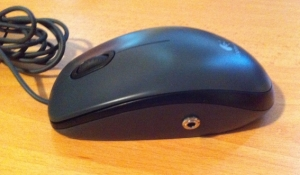
\includegraphics[width=1.0\textwidth]{fig/mouse13}
	\caption{Mouse adaptado para receber a interface P2 Jack de um acionador.}
	\label{fig:mouse}
\end{figure}

Como pode ser visto, o preço desses acionadores comerciais são bem elevados.
Algum deles possuem um mecanismo bem simples e ainda assim são vendidos a preços
absurdos. Por exemplo, o acionador~\cite{StringSwitch}, como mostrado no
vídeo~\cite{videoStringSwitch}, possui apenas uma simples corda que puxa uma
chave de fim de curso. O pino de referência é soldado no pino de refêrencia do
P2 Jack e o pino de estado da chave é soldado do pino se saída do P2 Jack.
Assim, quando o corda do acionador é puxada, os pinos de referência e saída do
P2 Jack são curto circuitados, ``simulando'' no P2 Jack os mesmos estados de
aberto e fechado da chave de fim de curso. Realizando pesquisas em sites como
MercadoLivre~\footnote{\url{https://www.mercadolivre.com.br/}}, é possível
encontrar a unidade de uma chave similar a utilizada nesse acionador custando 
cerca de R\$ 2.50. Já o pino de P2 jack custa cerca de R\$ 1. Com esses dois
materiais é possível construir um acionador semelhante ao discutido custando
menos de R\$ 10, valor bem abaixo dos U\$ 65 cobrado por esse acionador.

Na atual crise em que o Brasil se escontra, uma família de baixa renda, por
exemplo, difilcilmente iria adquidir um acionador externo devido ao elevedo
preço desses produtos, pois certamente comprometeria a renda mensal dessa
família.  Considernado que uma família possua a renda mensal de um salário
mínimo, e que esse salário está custe R\$ 954, e com o preço do dólar custando
R\$ 3.38, seria comprometido aproximadamente 23\% do salário dessa família caso
optassem por comprar esse acionador. Sendo assim, PCD de baixa renda ficam
impossibilitadas de adquirir esses produtos, excluindo-as de usufruir de
dispositivos que são voltadas para facilitar o uso de certos equipamentos que
não são adaptados para esse determinado público.

Nesse sentido, esta pesquisa tem como intuito apresentar uma solução para
diminuir a exclusão digital vivenciada pelas PCD, que muitas vezes não conseguem
utilizar aparelhos eletrônicos como \textit{smartphones} e computadores devido a
limitação de recursos que se adaptem às suas necessidades. Além disso a solução
proposta, apesar de ser voltada para o uso de uma determinada função em
aparelhos eletrônicos como computador, pode ser utilizada em outros dispositivos
que necessitem de uma interação através do pressionamento de um botão, como
ligar ou desligar televisores e lâmpadas. O uso de acionadores externos são bons
exemplos de dispositivos que auxiliam na utilização de diversos dispositivos,
porém como grande parte dos acionadores disponíveis no mercado possuem um custo
muito elevado, há a necessidade da solução proposta ser mais acessível
economicamente para que mais PCD possam ter acesso a essas ferramentas que
auxiliam o uso de tarefas em dispositivos que normalmente não possuem interfaces
alternativas de controle. 
 
\subsection{Trabalhos Relacionados}
A ideia de ajudar PCD a utilizar aparelhos eletrônicos com o auxílio de 
acionadores externos é alvo de inúmeras pesquisas. Uma grande parte dessas
pesquisas foca em auxiliar tarefas de controle das funções básicas do
\textit{mouse} de um computador. Para controlar o ponteiro do \textit{mouse}, o
método mais utilizado é o que utiliza os movimentos da cabeça ou dos olhos. Para
esse tipo de abordagem há uma certa dificuldade em emular a função de clique.
Geralmente, para essa determinada função,  é utilizada o \textit{dwelltime}, 
um método que utiliza um tempo específico em segundos em que o ponteiro do mouse
fica sobre um determinada área da tela para realizar  o clique. Por exemplo, se
o usuário posicionar o ponteiro sobre o ícone de fechar uma aba de um navegador
por um determinado tempo, irá ser chamado a função de clique sob esse ícone,
fechando essa aba do navegador. Um dos problemas desse tipo de abordagem está no
fato de que o usuário é obrigado a ficar com a cabeça os com os olhos parados
em uma determinada posição por algum tempo para que a função de clique seja
ativada. Isso gera uma um certo incômodo e fadiga no pescoço e nos olhos, para o 
caso de o  ponteiro ser controlado com os movimentos da cabeça e dos olhos, 
respectivamente, além de ,naturalmente, aumentar o tempo de utilização a medida em
que o número de tarefas realizadas também aumentar.

Devido isso há diversas pesquisas que tentam solucionar esse problema através de
métodos alternativos para a emulação do clique do \textit{mouse}.
Em~\cite{Aanand18} foi proposto um algoritmo chamado de OptiDwell para emular a
função de clique. Esse algoritmo utiliza o mesmo princípio do
\textit{dwelltime}, mas com a difirença de que o usuário sabe exatamente quando
o evento de clique irá acontecer. No \textit{dwelltime} o usuário sabe qual é o
tempo especifico em que o ponteiro deve ficar sobre uma área que se deseja
clicar, mas não tem a noção exata desse tempo. Por exemplo, se a pessoa deseja
pausar um vídeo no YouTube, ela deve posicionar o ponteiro sobre o ícone de
pause do vídeo e esperar o tempo de 2 segundos --- caso o \textit{dwelltime}
esteja configurado para 2 segundos --- para que a função de clique seja ativada.
Se em 1.99 segundos após ponteiro ficar sobre o ícone de pause, o cursor sair
dessa posição, a função de clique não é chamada, sendo necessário, então,
posicionar o ponteiro novamente em cima do ícone desejado. Com o método
proposto, o usuário tem uma noção mais exata do tempo para que a função de clique
seja realizada. O usuário sabe que o clique está para ser realizado através da
mudança de cor do ícone onde o ponteiro está posicionado. Por exemplo, se a
pessoa deseja clicar em uma letra no teclado virtual disponibilizado em vários
sistemas operacionais, essa letra ficará trocando de cor ao longo do tempo,
quando estiver em uma determinada cor, a função de clique será chamada, além de
ser ativado som de estalo (clique). Com isso a pessoa tem uma noção mais precisa
do tempo para realizar o clique, através de um \textit{feedback} visual e
sonoro. Contudo, o tempo de execução dessa função continua sendo um problema,
pois o tempo de execução de tarefas simples, como a digitação, demanda mais
tempo do que outros métodos alternativos.

O trabalho proposto em~\cite{Skim10} utiliza um acionador baseado em dois
sensores ópticos: um LED (do inglês, ~\textit{light emitting diode})
infravermelho emissor e um receptor. Esse método levou em consideração o
clique simples e duplo, descartando a implementação da função ``clicar e
arrastar''. Os sensores foram posicionados bem próximos de um dos olhos do
usuário e através da tensão no LED infravermelho receptor foi possível
identificar se a pessoa estava de olho aberto ou fechado. Quando o usuário fica
de olho fechado há um certo sinal de tensão no LED emissor, mas quando o usuário
abre o olho, a o sinal infravermelho refletido no olho aberto geral uma tensão
bem abaixo da tensão percebida quando a pessoa está com o olho fechado. Com
isso foi possível detectar os eventos de clique identificando os piscar dos
olhos --- transição aberto-fechado dos olhos --- do usuário. A detecção foi
baseada na amplitude do sinal de tensão do LED receptor e o tempo em que o
usuário ficava de olho fechado, evitando que o sistema identificasse um clique
de involuntário quando a pessoa piscasse de forma natural. Esse acionador
construído para realizar o clique de um \textit{mouse} é bastante interessante,
porém, como descrito em~\cite{Batista17}, onde foi elaborado um acionador que
utiliza esse mesmo princípio de funcionamento, pode acarretar em uma série de
reconhecimentos equivocados de clique devido o sensor utilizado ser bastante
influenciado pelas condições do ambiente, como iluminação de lâmpadas
fluorescentes e do sol.

O método proposto em~\cite{Karimullah02} utilizou o reconhecimento de voz para
controlar o ponteiro do \textit{mouse} e o evento de clique simples. Para mover 
o ponteiro foi implemento o reconhecimento para quatro comandos: \textit{move
left, move right, move up, move down} e \textit{stop} para mover o cursor para
esquerda, direita, cima, baixo e parar o cursor, respectivamente. Quando o
usuário realiza um comando para mover o cursor --- \textit{move right}, por 
exemplo ---, o ponteiro começa a se mover a 20 \textit{pixels} por segundo na
direção dado no comando e só para de se movimentar quando for reconhecido o
camando \textit{stop}. Em relação ao evento de clique, foi implementado apenas o
clique simples do \textit{mouse}, sendo necessário realizar o comando 
\textit{click} para que o sistema emule essa função. O trabalho proposto é
bastante interessante, mas pode apresentar problemas, caso o usuário desejar
mover o cursor para uma determinada área que esteja muito próxima da posição
atual do ponteiro e não houver tempo suficiente entre os comandos de mover e
parar o cursor para que o ponteiro fique exatamente sobre a área desejada.
Contudo, se a função de clique proposta pelo autor for combinada com outros
métodos alternativos de controle de \textit{mouse} que utilizam o
\textit{dwelltime}, o tempo de realização das tarefas que envolvem o clique
seria mais otimizado.

Há trabalhos que utilizam acionadores baseados em sinais obtidos por
eletromiografia (EMG) --- um método de registro da tividade de um músculo quando
realiza contração~\cite{Amadio07} --- para implementar a função de clique.
Em~\cite{Pinheiro12}, por exemplo, foi implementado a função de clique simples e
duplo através de sinais de EMG. Os eletrodos que capturam os sinais elétricos
foram colocados no músculo frontal. A Figura~\ref{fig:frontal} mostra a
localização do músculo frontal. Para o clique simples, basta o usuário levantar
as sobrancelhas. Já para o clique duplo, a sobrancelha deve ser levantada duas
vezes de forma consecutiva. Assim, o sinal elétrico capturado pelo circuito de
EMG é convertido nesses dois eventos de clique.

\begin{figure}[H]
	\centering
	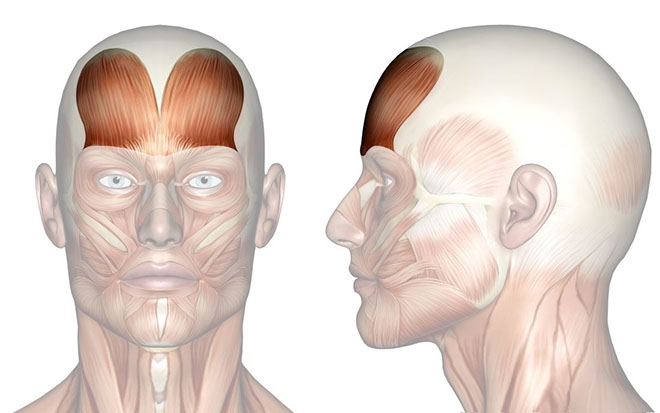
\includegraphics[width=0.5\textwidth]{fig/frontal}
	\caption{Músculo frontal.}
	\label{fig:frontal}
\end{figure}

Já em~\cite{Kaushik12} foi proposto um acionador que permitia controlar o
movimento do ponteiro do mouse assim como as funções de clique esquerdo e
direito, através de EMG e meconomiografia (MMG). A MMG, é uma técnica
não-invasiva que registra as vibrações ou sons produzidos pelo músculo
esquelético ao se contrair~\cite{Vaz99}. Os eletrodos de EMG foram colocados nos
músculo masseter e risório, mostrados na Figura~\ref{fig:masseter} e na
Figura~\ref{fig:risorio}, respectivamente. %Para o MMG foi utilizado um
\begin{figure}[H]
    \centering
    \begin{minipage}{.5\textwidth}
        \centering
        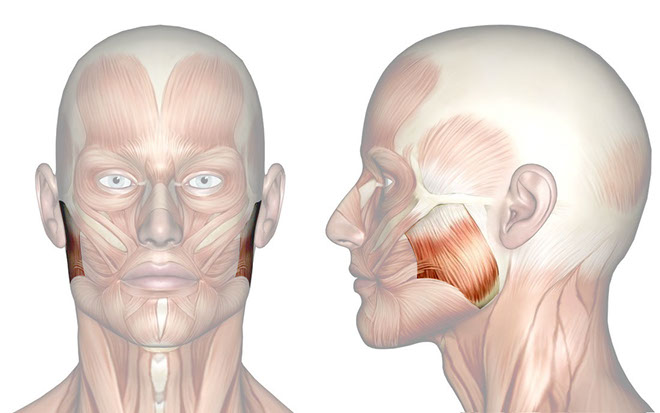
\includegraphics[width=0.9\linewidth, height=0.2\textheight]{fig/masseter}
        \caption{Músculo masseter.}
        \label{fig:masseter}
    \end{minipage}%
    \begin{minipage}{0.5\textwidth}
        \centering
        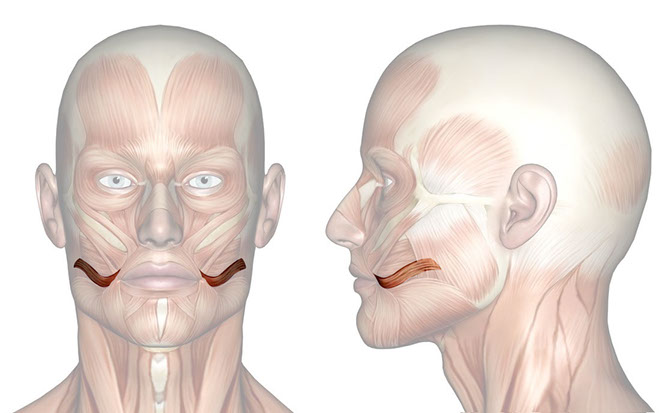
\includegraphics[width=0.91\linewidth, height=0.2\textheight]{fig/risorio}
        \caption{Músculo risório}
        \label{fig:risorio}
    \end{minipage}
\end{figure}
Para o MMG foi utilizado um Piezoelétrico --- um transdutor que sob estresses
mecânicos, como vibrações e compressões, gera sinais elétricos --- que foi
colocado no músculo platisma localizado no pescoço, como mostrado na
Figura~\ref{fig:platisma}. As palavras \textit{up, down, left} e \textit{right}
foram usadas para controlar o ponteiro do \textit{mouse}. Já para a função de
clique esquerdo e direito, foram utilizadas as palavras \textit{left click} e
\textit{right click}, respectivamente.
\begin{figure}[H]
	\centering
	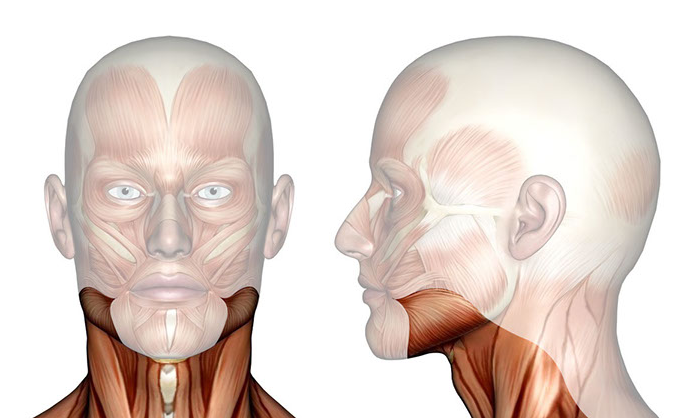
\includegraphics[width=0.5\textwidth]{fig/platisma}
	\caption{Músculo platisma.}
	\label{fig:platisma}
\end{figure}

O trabalho~\cite{Simpson08} que utiliza os movimentos da cabeça para controlar o
ponteiro do \textit{mouse}, utilizou um acionador muito interessante que
utilizava os sinais de um acelerômetro para realizar os eventos de clique. O
sensor acelerômetro foi posicionado atrás da orelha, de modo semelhante como
ficam posicionados alguns aparelhos auditivos que ajudam pessoas que possuem
dificuldade de audição a melhorar sua capacidade auditiva. Esse acionador é
dividido em dois módulos: transmissor e receptor. O módulo transmissor é o que
fica, de fato, posicionado atrás da orelha do usuário. Já o receptor fica
conectado diretamente no computador via USB. Os módulos se comunicam entre si
utilizando sinais de rádiofrequência. Para ativar a função de clique, o usuário
deve realizar uma pressão entre os dentes superiores e inferiores, de forma
semelhante como funciona a mastrigação. Portanto, quando o usuário realiza essa
pressão entre os dentes, é enviado um sinal do módulo transmissor, para o
receptor que, por sua vez, passa o comando referente ao clique para o computador
via USB. O sensor é capaz de distinguir o comando de clique através da pressão
entre os dentes, da vibração causado no sensor quando o usuário movimenta a
cabeça e até mesmo da vibração causada pelo ato de abrir a boca ao falar ou
bocejar. Isso evita que cliques do \textit{mouse} sejam detectados de forma
equivocada, tornando o acionador mais confiável para o função do clique. 

Já em~\cite{Antunes16} foi utilizado os movimentos da cabeça capturados ao longo
de \textit{frames} por uma \textit{webcam} para controlar o ponteiro do mouse,
sendo que, para o evento de clique, foi utilizado o auxílio de um acionador
baseado em pressão. O acionador é do tipo pedal e é bem semelhante aos pedais
utilizados por guitarristas para realizar distorções em notas musicais
produzidas pela guitarra. O acionador possui uma comunicação direta com o
computador através da tecnologia Bluetooth. Portanto, para realizar um clique no
computador, o usuário deve pressionar com os pés o acionador. Quando o acionador
é pressionado, o comando de clique é enviado via Bluetooth para o computador.
Com isso uma que tenha os movimentos dos membros inferiores preservados,
consegue utilizar a função de clique no computador sem a necessidade de utilizar
a mãos. 

%\section{Objetivos}

%\section{Síntese de Conteúdo}


\end{chapter}

\begin{chapter}{Referencial Teórico}
Este capítulo tem como objetivo apresentar o referencial teórico das ferramentas
mais importantes para o desenvolvimento do dispositivo proposto neste trabalho,
como i) piezoeletricidade; ii) amplificadores operacionais; iii) Conectores de
áudio; iv) ferramenta de desenvolvimento de placas de circuito impresso; v)
captura de sinais através da interface de áudio do computador; e, finalmente vi)
ferramenta para a emulação dos eventos de clique do \textit{mouse}.

\begin{section}{Piezoeletricidade}

Há certos elementos capazes de converter uma grandeza física em outra. Por
exemplo, transformar temperatura em tensão elétrica. Esses elementos são
chamados de transdutores~\cite{william}. Um grande exemplo de transdutor é o
microfone, que é capaz de converter o som, uma onda mecânica, em sinais
elétricos que são amplificados posteriormente por um circuito. %Muitas vezes
%transdutores são chamados de sensores, porém esta denominação não é correta,
%pois, segundo~\cite{usher}, sensor é um dispositivo capaz de medir uma grandeza
%física, como é o caso do termômetro que realiza a medição de temperatura. 

Além disso, há certos transdutores que são capazes de converter mais de uma
grandeza física, como é o caso do transdutor piezoelétrico. Esse transdutor
opera sob o fenômeno físico conhecido como piezoeletricidade e é bastante
utilizado em diversas aplicações. Seu principio de funcionamento é dividido em
efeito piezoelétrico direto e reverso, os quais são brevemente descritos a
seguir.
  
\begin{subsection}{Efeito Piezoelétrico Direto}

O efeito piezoelétrico direto refere-se a capacidade de um material gerar tensão
elétrica quando submetido a estresses mecânicos como compressão ou
vibração~\cite{jaffe2012piezoelectric}. Muitos aparelhos eletrônicos utilizam
essa propriedade da piezoeletricidade. Por exemplo, piezos são bastantes
utilizados na indústria como uma ferramenta que ajuda a detectar a presença de
objetos em determinadas áreas. Quando há algum objeto sobre uma área desejada,
o peso desse objeto realiza uma força de compressão sobre o material
piezoelétrico, produzindo uma diferença de potencial elétrico. Dessa
forma, uma máquina pode ``perceber'' que há um objeto sobre a área desejada e
pode então realizar a sua função pré-programada. %É importante perceber que o
%piezo converte, nesse caso a força peso causada pela massa do objeto, em uma
%energia elétricacapaz de ser .
  
\begin{figure}[!h]
	\centering
	\begin{minipage}[c]{\textwidth}
	\centering
	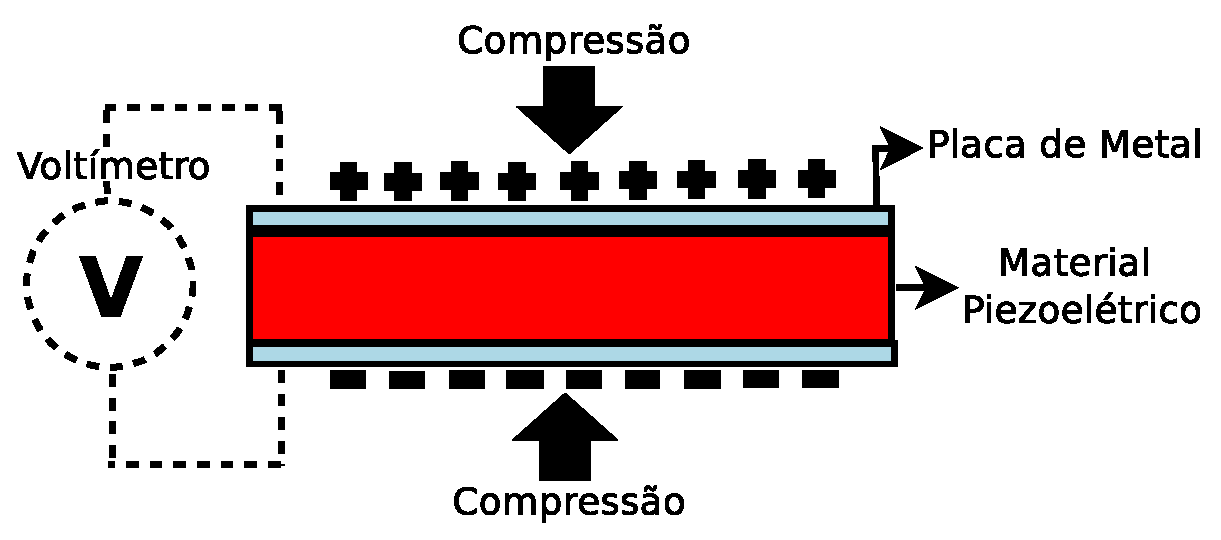
\includegraphics[width=0.8\linewidth]{fig/EfeitoPiezoEletricoDireto}
	\caption{Efeito piezoelétrico direto.}
	\vspace{-1cm}
	\caption*{\textbf{Fonte: }Elaborada pelo autor.}
	\label{fig:direto}
	\end{minipage}
\end{figure}

\vspace{-0.5cm}
A Figura~\ref{fig:direto} mostra o princípio de funcionamento do efeito
piezoelétrico direto. Um material piezoelétrico --- um cristal de quartzo, por
exemplo --- é posicionado entre duas placas de metal. Para ocorrer a geração de
energia elétrica, é necessário algum tipo de estresse mecânico no material, como
compressão ou vibração. Quando as placas de metal são pressionadas, ocorre uma
diferença de potencial elétrico na superfície das placas como consequência do
chamado efeito piezoelétrico direto.  É possível inclusive armazenar a
energia gerada pela compressão do material piezoelétrico e utilizá-la para
alimentar circuitos elétricos, ao invés de usar baterias~\cite{twitter}. 

\end{subsection}


\begin{subsection}{Efeito Piezoelétrico Reverso}

A Figura~\ref{fig:reverso} ilustra o princípio de funcionamento do efeito
piezoelétrico reverso, processo contrário ao efeito piezoelétrico direto. Dadas
duas placas de metal separadas por um material piezoelétrico, é possível gerar
perturbações mecânicas nessas placas. Para isso, é necessário aplicar uma
diferença de potencial elétrico nas placas que vibram proporcionalmente a tensão
aplicada~\cite{Lin12}. Ondas de sons audíveis podem ser geradas a partir das
vibrações das placas de metal, mas para que isso ocorra, as placas devem
necessariamente vibrar em uma faixa de frequência entre 20~Hz e 20~kHz (faixa de
frequência audível ao ser humano).


\begin{figure}[!h]
	\centering
	\begin{minipage}[c]{\textwidth}
	\centering
	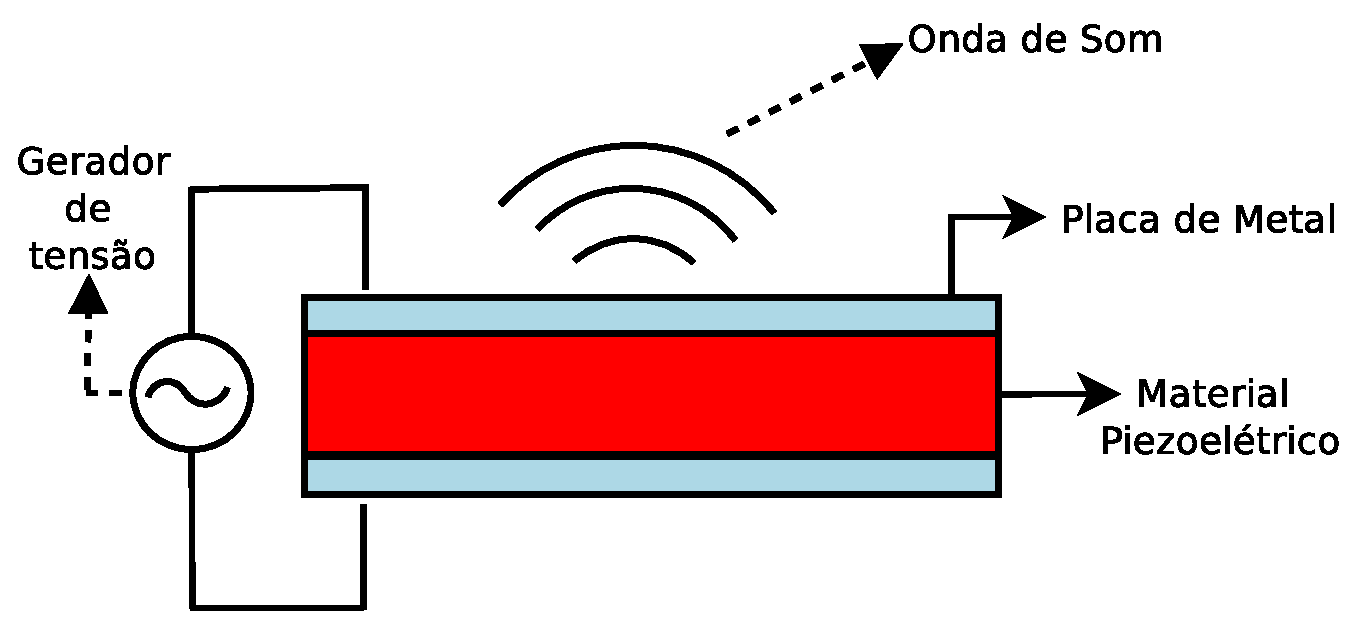
\includegraphics[width=0.8\linewidth]{fig/EfeitoPiezoEletricoReverso}
	\caption{Efeito piezoelétrico reverso.}
	\vspace{-1cm}
	\caption*{\textbf{Fonte: }Elaborada pelo autor.}
	\label{fig:reverso}
	\end{minipage}
\end{figure}

\vspace{-1cm}
Muitos aparelhos eletrônicos utilizam o efeito piezoelétrico reverso. Os sons de
sinalizações emitidos por computadores ao serem ligados (\textit{beeps}) ou
quando há algum tipo de problema no funcionamento no computador, são gerados por
um dispositivo chamado \textit{buzzer}, o qual é um bom exemplo de utilização do
efeito piezoelétrico reverso.  Até mesmo alguns sonares utilizam o princípio
desse fenômeno da piezoeletricidade, onde é aplicada uma tensão modulada por PWM
(do inglês \textit{pulse with modulation}) em um material piezoelétrico que
emite um sinal ultrassom. Alguns desses instrumentos ultrassônicos são
utilizados na área médica na realização de cortes em cirurgias, como a
maxilofacial onde é necessário realizar cortes em tecidos
ósseos~\cite{Carvalho17}. 
 
\end{subsection}

\end{section}

\begin{section}{Amplificadores Operacionais} 

O circuito eletrônico conhecido como amplificador operacional é um componente
muito importante em circuitos elétricos que realiza operações especiais de
processamento de sinais~\cite{Richard2000}. 

\begin{figure}[!h]
	\centering
	\begin{minipage}[c]{\textwidth}
	\centering
	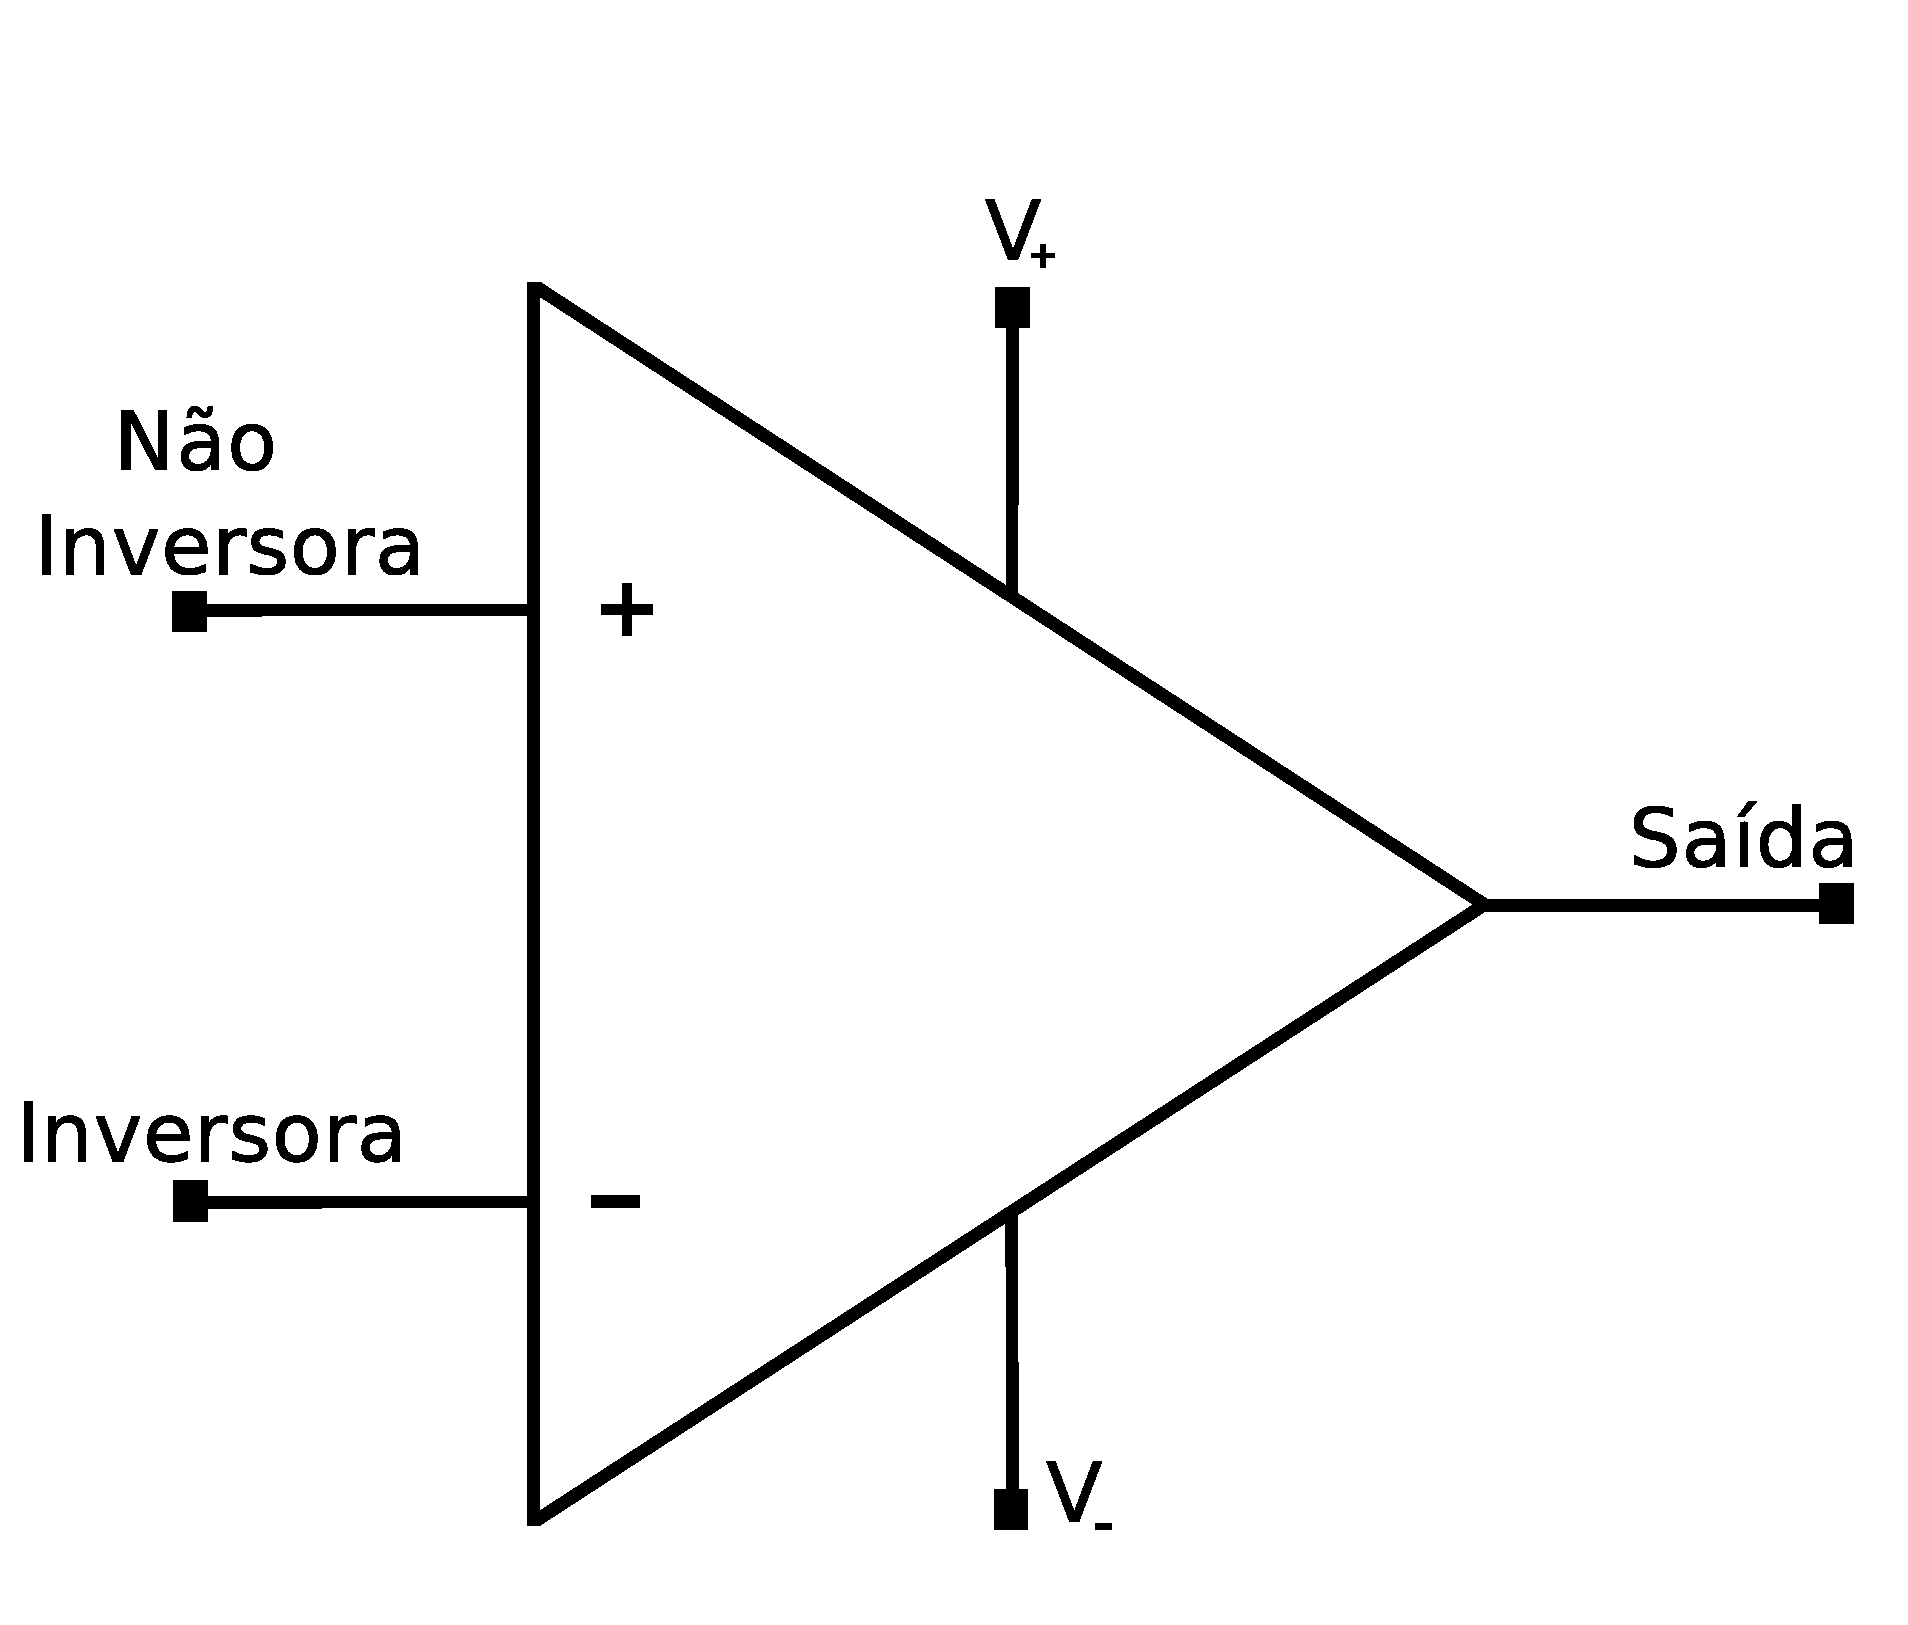
\includegraphics[width=0.4\linewidth]{fig/opamp}
	\caption{Representação de um amplificador operacional.}
	\vspace{-1cm}
	\caption*{\textbf{Fonte: }Elaborada pelo autor.}
	\label{fig:opamp}
	\end{minipage}
\end{figure}

O amplificador operacional ilustrado na Figura~\ref{fig:opamp} possui dois
terminais de alimentação, duas entradas, inversora e não inversora ($V_{-}$ e
$V_{+}$), e uma saída. A entrada não inversora é convencionalmente representada
pelo símbolo ``+'' e a entrada inversora é representada pelo símbolo ``-''.
Alguns autores omitem a representação dos terminais de alimentação por
considerarem desnecessários e tenderem a sobrecarregar visualmente os esquemas
de circuitos, tornando-os mais difíceis de serem interpretados. Contudo, fica
subentendido que os terminais de alimentação fazem parte do circuito, embora
muitas vezes não sejam mostrados.

A partir de várias combinações de resistores nos terminais do amplificador
operacional, é possível executar funções muito úteis com os sinais de entrada, 
como multiplicação por um fator constante, soma, mudança de fase e
subtração~\cite{Nilson09}. Outra função bastante importante que pode ser
implementada com amplificadores operacionais é a comparação de sinais. Dado dois
sinais, um em cada entrada, a saída é determinada a partir de uma comparação de
intensidade entre os dois sinais de entrada~\cite{Terrell96}.  
 

\begin{figure}[!h]
	\centering
	\begin{minipage}[c]{\textwidth}
	\centering
	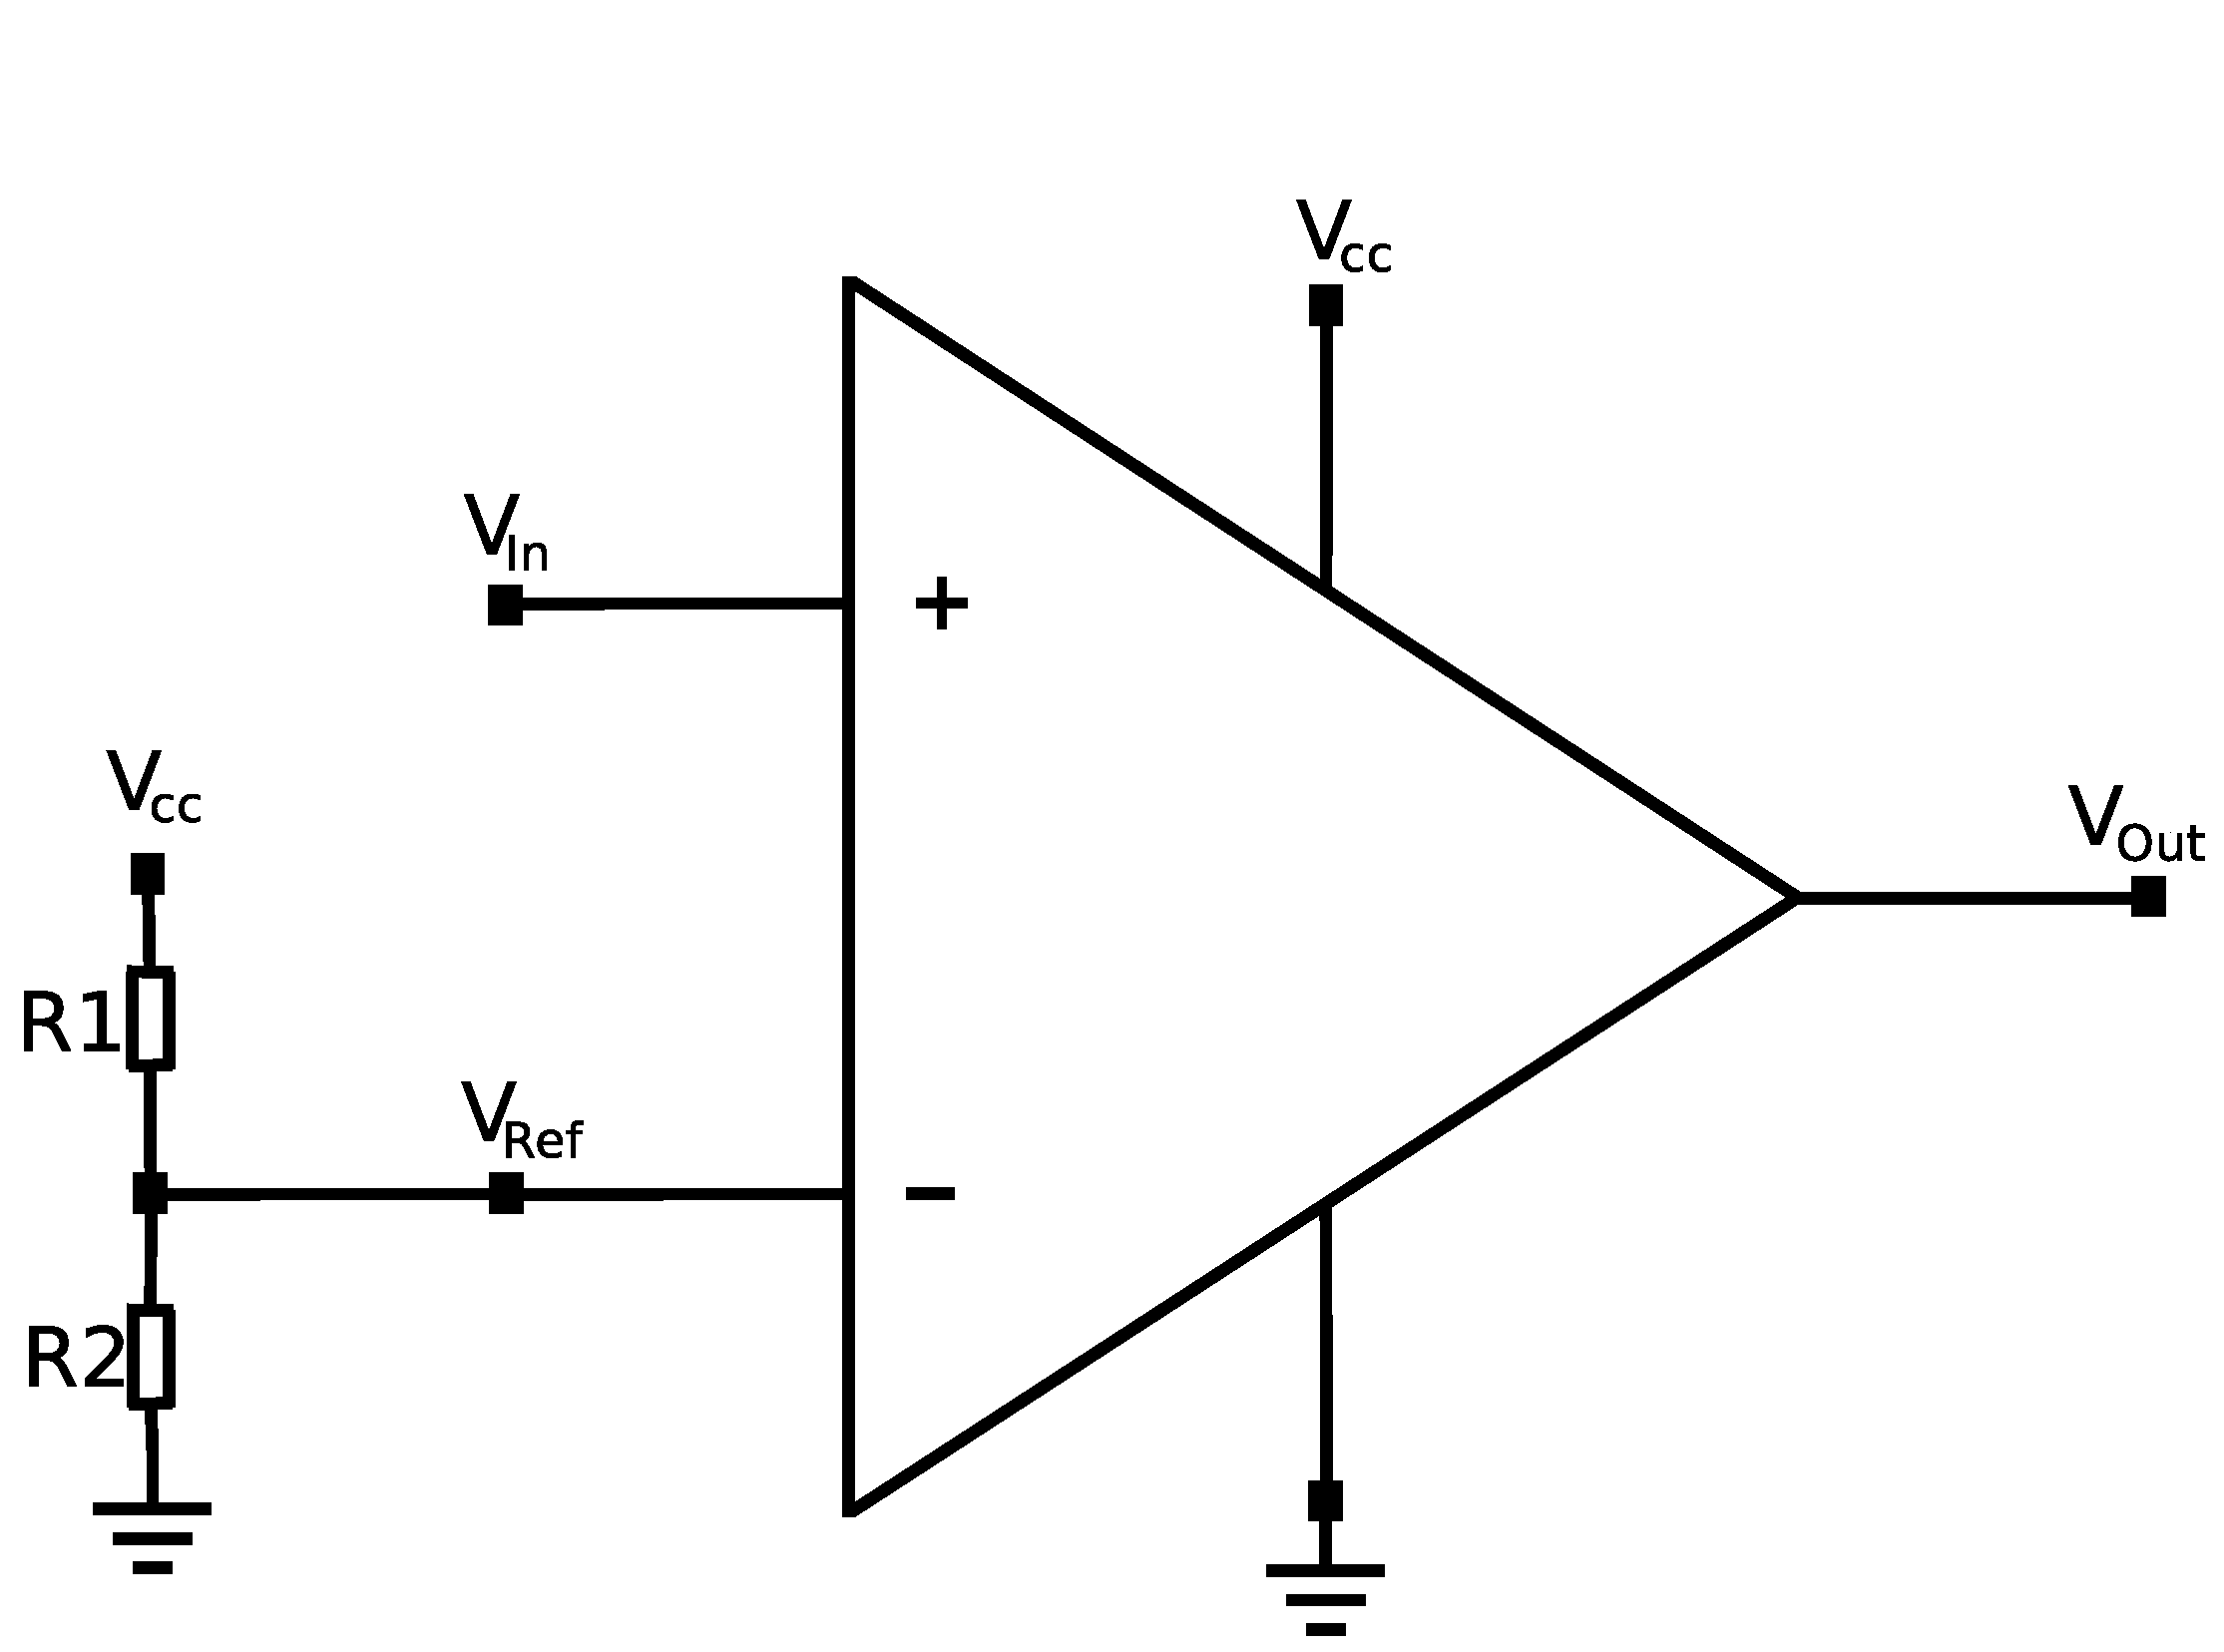
\includegraphics[width=0.45\linewidth]{fig/nao_inversor}
	\caption{Circuito comparador não inversor.}
	\vspace{-1cm}
	\caption*{\textbf{Fonte: }Elaborada pelo autor.}
	\label{fig:comparador1}
	\end{minipage}
\end{figure}

A Figura~\ref{fig:comparador1} mostra um comparador de tensão utilizando a
configuração não inversora. Nessa configuração de comparação, uma tensão como
referência ($V_{Ref}$) é utilizada na entrada inversora. A
Figura~\ref{fig:sinal1} mostra o comportamento dos sinais utilizando essa
configuração.

\begin{figure}[!h]
	\centering
	\begin{minipage}[c]{\textwidth}
	\centering
	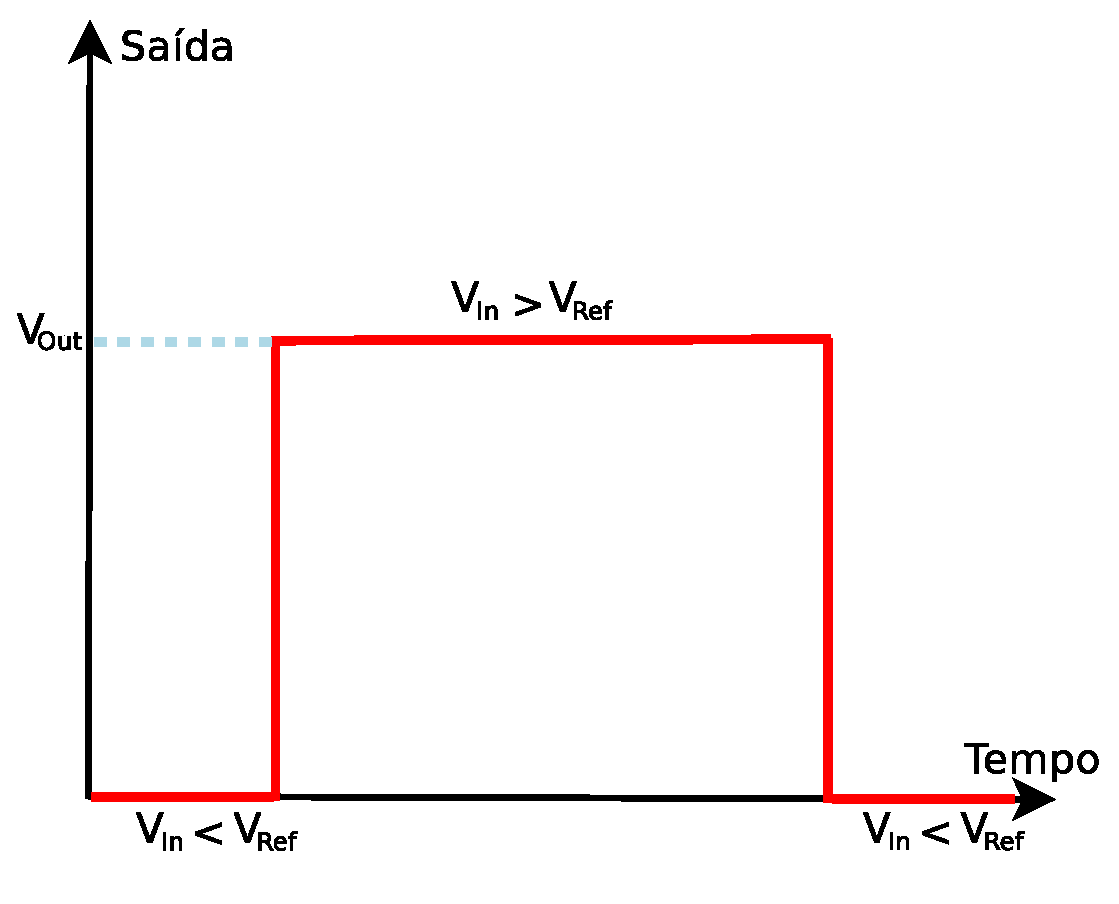
\includegraphics[width=0.55\linewidth]{fig/comparador_nao_inversor}
	\caption{Comportamento do sinal de saída do comparador não inversor.}
	\vspace{-1cm}
	\caption*{\textbf{Fonte: }Elaborada pelo autor.}
	\label{fig:sinal1}
	\end{minipage}
\end{figure}

Enquanto a tensão de referência for maior que o sinal da entrada na porta não
inversora ($V_{In}$), a saída ($V_{Out}$) tende para 0~V. Contudo, quando a
tensão da entrada não inversora é maior que a tensão de referência, a saída
tende para a magnitude da tensão utilizada como alimentação do amplificador
operacional ($V_{cc}$). Por exemplo, se o amplificador for alimentado com 15~V a
saída desse componente se aproximaria de 15~V, porém nunca chegaria a essa
magnitude de tensão. Idealmente, o valor de saída deveria ser exatamente 15~V,
porém na prática isso não acontece devido a diversos fatores físicos do
componente.

\begin{figure}[!h]
	\centering
	\begin{minipage}[c]{\textwidth}
	\centering
	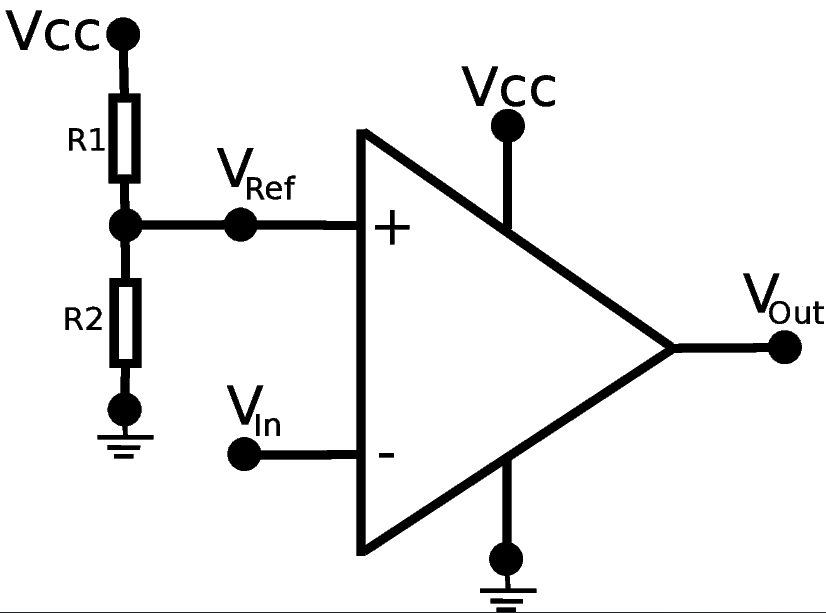
\includegraphics[width=0.5\linewidth]{fig/inversor}
	\caption{Circuito comparador não inversor.}
	\vspace{-1cm}
	\caption*{\textbf{Fonte: }Elaborada pelo autor.}
	\label{fig:comparador2}
	\end{minipage}
\end{figure}
\break
Já a Figura~\ref{fig:comparador2} mostra um comparador de tensão utilizando a
configuração inversora. Nessa configuração, também é utilizada uma tensão de
refêrencia, porém é colocada na entrada não inversora. O comportamento dos sinais
utilizando a configuração inversora é mostrado na Figura~\ref{fig:sinal2}. 


\begin{figure}[!h]
	\centering
	\begin{minipage}[c]{\textwidth}
	\centering
	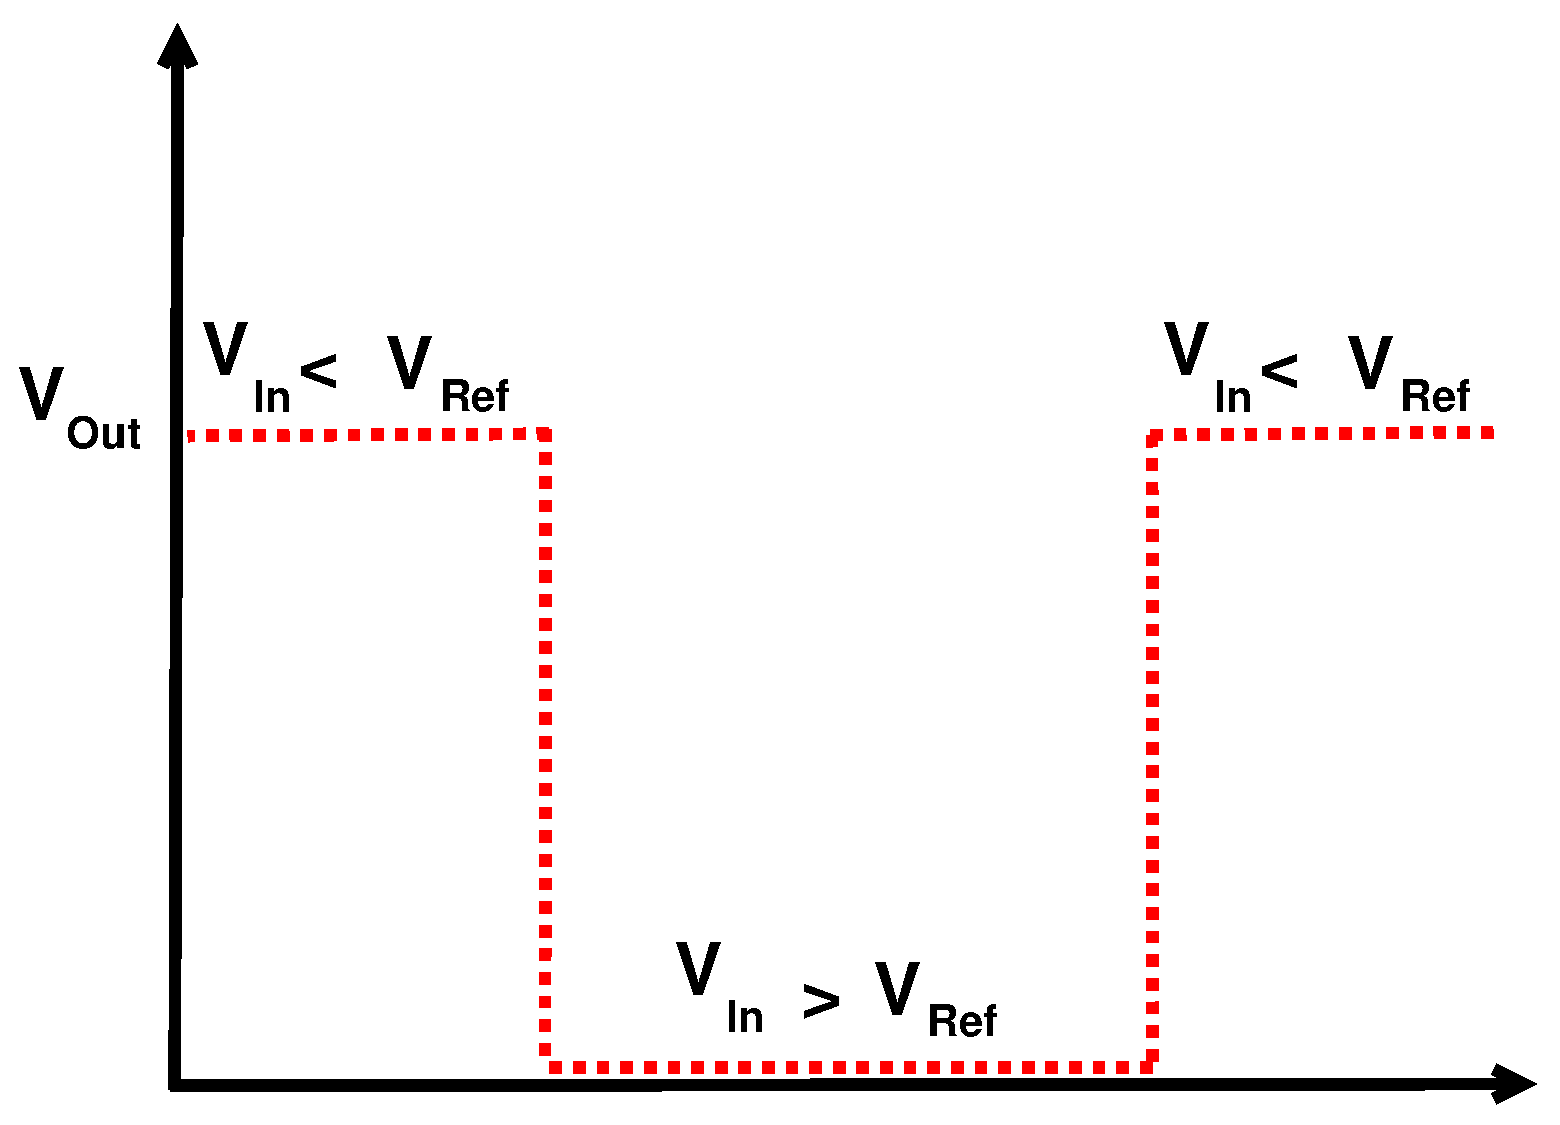
\includegraphics[width=0.55\linewidth]{fig/comparador_inversor}
	\caption{Comportamento do sinal de saída do comparador inversor.}
	\vspace{-1cm}
	\caption*{\textbf{Fonte: }Elaborada pelo autor.}
	\label{fig:sinal2}
	\end{minipage}
\end{figure}

A configuração de comparador inversor ocorre, como o próprio nome sugere, um
comportamento oposto ao comparador não inversor. Enquanto a tensão de referência
é maior que a tensão da entrada, a saída tende para a magnitude da tensão de
alimentação do amplificador operacional. Já quando ocorre o contrário,  a tensão
da saída tende para 0~V.

\end{section}


\begin{section}{Conectores de Áudio TS e TRS}

Sinais de áudio podem ser transmitidos através de vários tipos de conectores.
Por exemplo, é possível reproduzir os sinais de áudio produzidos por uma
guitarra para uma caixa acústica amplificada. Geralmente, utiliza-se o conector
P10 para realizar a transmissão de áudio da guitarra para a caixa acústica. Já
para fones de ouvidos, o conector P2 é mais comumente utilizado. Segundo uma
matéria disponível na BBC News~\cite{BBC}, o conector P2 é utilizado desde o
século XIX, mas nessa época eram mais utilizados para conectar e desconectar 
conexões em painés telefônicos antigos. Os conectores mais utilizados são os 
conectores TS e TRS, também conhecidos como conectores Jack, que serão 
brevemente descritos a seguir.  
\newpage
O TS é um conector utilizado para transmitir sinais analógicos e são mais
utilizados natransmissão de áudio. Esse conector é chamado de TS por ser as
iniciais das palavras Tip e Sleeve. Há diversos tamanhos de
conectores TS e são comercializados com diferentes diâmetros, como 2,5~mm,
3,5~mm e 6,35~mm. A Figura~\ref{fig:ts} mostra a ilustração de um conector TS.
Esse conector possui somente um canal de transmissão de sinal analógico, por
isso é um conector mono~\cite{ts}. O TS possui dois pinos que são separados
entre si por um anel isolante. O pino Tip que  fica localizado no final do
conector é utilizado para realizar a  transmissão do sinal. Já o pino Sleeve é
responsável por ser a referência (GND, \textit{ground}, ou terra) do conector.

O TRS, mostrado na Figura~\ref{fig:trs}, também é um conector utilizado para
transmissão de sinais analógicos. Esse conector às vezes é chamado de P3, por
possuir três pinos, porém este nome está tecnicamente incorreto pois a
nomenclatura é denominada de acordo com o diâmetro de cada conector. Sendo assim
a nomenclatura P2, por exemplo, podendo ser tanto TS quanto TRS,  refere-se a
conectores com diâmetro de 3,5~mm, assim como P10 refere-se a conectores de
6,35~mm. 

%\begin{figure}[!h]
%	\centering
%	\begin{minipage}[c]{\textwidth}
%	\centering
%	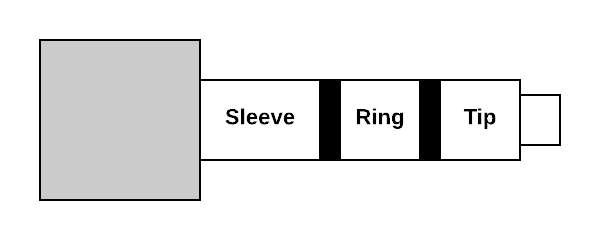
\includegraphics[width=0.9\linewidth]{fig/trs}
%	\caption{Conector TRS.}
%	\label{fig:TRS}
%	\end{minipage}
%\end{figure} 

%%casso
%\begin{figure}
%\centering
%\begin{subfigure}{.4\textwidth}
%  \centering
%  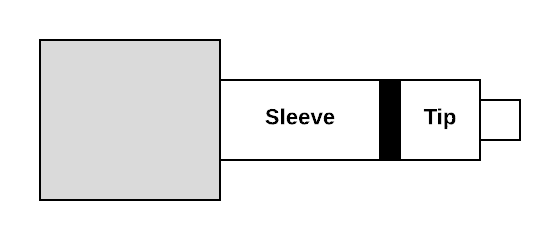
\includegraphics[width=1\linewidth, height=0.2\textheight]{fig/ts}
%  \caption{Conector TS.}
%  \label{fig:ts}
%\end{subfigure}%
%\begin{subfigure}{0.4\textwidth}
%  \centering
%  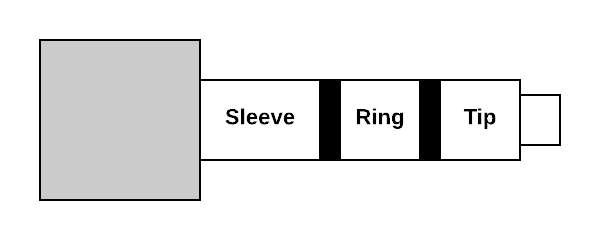
\includegraphics[width=1\linewidth, height=0.2\textheight]{fig/trs}
%  \caption{Conector TRS.}
%  \label{fig:trs}
%\end{subfigure}
%\caption{Conectores de áudio.}
%\label{fig:conector}
%\end{figure}

\begin{figure}
	\centering
	\subfloat[Conector TS.\label{fig:ts}]  {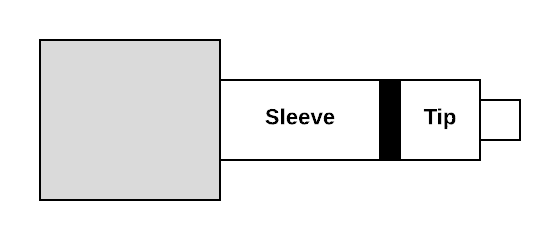
\includegraphics[width=0.50\linewidth]{fig/ts}}
	\subfloat[Conector TRS.\label{fig:trs}]{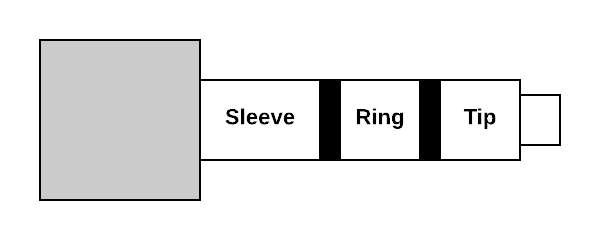
\includegraphics[width=0.50\linewidth]{fig/trs}}
	\caption{Conectores de áudio.}
	\vspace{-1cm}
	\caption*{\textbf{Fonte: }Elaborada pelo autor.}
	\label{fig:conector}
\end{figure}

O conector TRS possui três pinos que, assim como o TS, são separados 
entres si por anéis isolantes. Contudo, o TRS pode transmitir dois sinais
analógicos simultaneamente, sendo, portanto, um conector estéreo~\cite{ts}. O
pino Sleeve, ou GND, é a referência do conector. O pino Ring, também chamado de
Right (canal direito da transmissão) é o  pino central do conector. Já Tip,
pino localizado no final do conector, também é conhecido por Left, pois é 
responsável por transmitir um sinal pelo canal esquerdo.

\break 
É possível transformar um conector TRS em TS, ou seja, transformar um conector
estéreo em mono. Para isso, é necessário realizar um curto-circuito entre os
pinos Ring e Tip do conector estéreo. Quando um sinal é enviado para o Ring e
Tip, como eles estão curto circuitados, os dois canais transmitem o mesmo
sinal em somente um canal, agindo como um conector TS.


\end{section}


\begin{section}{Ferramentas de Desenvolvimento de Placas de Circuito Impresso}

Para o desenvolvimento de placas de circuito impresso (PCB, do inglês
\textit{printed circuit board}), primeiramente é
preciso desenvolver o \textit{layout} do circuito que deseja-se transferir
para a placa. Para realizar essa tarefa é necessário a utilização de um
\textit{software} EDA (do inglês, \textit{electronic design automation}). O
Eagle~\cite{eagle} é um dos \textit{software} EDA mais utilizados para o
desenvolvimento de placas de circuito impresso, contudo possui a desvantagem de
não ser um \textit{software} livre, sendo liberado gratuitamente apenas para uso
pessoal e não comercial. Além disso, a versão gratuita possui uma quantidade
limitada de ferramentas de desenvolvimento. Para ter acesso a essas ferramentas,
o desenvolvedor tem que adquirir uma assinatura que pode ser mensal ou anual. Os
valores dessa assinatura variam de R\$~52,91 a
R\$~3.227,40~\cite{EagleAssinatura}. 
 
No entanto, existem ferramentas EDA que são de código aberto e totalmente
gratuitas. O Kicad~\cite{kicad} é o  \textit{software} de código aberto e
gratuito mais utilizado entre os desenvolvedores. Essa ferramenta oferece
recursos necessários para o desenvolvimento de quase todo tipo de projeto.
Obviamente, devido à vasta quantidade de componentes eletrônicos existentes no
mundo, não existem bibliotecas para todos os componentes possíveis. Contudo, há
a possibilidade de desenvolvimento de bibliotecas próprias, sendo possível
disponibilizá-las em repositórios gratuitos, como o GitHub~\cite{github}, para
que qualquer pessoa possa utilizá-la em projetos pessoais.  
\end{section}


\begin{section}{Captura de Áudio}

Para o desenvolvimento de uma aplicação de captura ou reprodução de áudio é
imprescindível a utilização de alguma API. Uma API (do inglês,
\textit{application programing interface}) é uma interface que define o contrato
para que duas aplicações se comuniquem entre si~\cite{API17}. A utilização de
uma API pode simplificar o desenvolvimento de aplicações, contudo há algumas
limitações, como linguagem e plataforma utilizada. 

Existem várias APIs para o desenvolvimento de aplicações de áudio. Agumas APIs
são nativas do sistema operacional, portanto cada sistema operacional possui
APIs específicas. A grande desvantagem de utilizar APIs nativas de um
determinado sistema operacional é questão da portabibidade. Para a utilização da
mesma aplicação em outro sistema operacional, é necessário a reescrita do código
utilizando um API suportada pelo sistema operacional onde deseja-se executar a
aplicação. Isso é um grande problema, pois reescrever um código praticamente do
início, uma vez que uma nova API deve ser utilizada, demanda tempo e muitas vezes
recursos finaceiros adicionais para o desenvolvimento do projeto.


A camada de áudio de sistemas operacionais baseados em Linux, por
exemplo, possui o ALSA~\cite{alsa} e também o OSS~\cite{oss} (mais antigo e
menos utilizado) como
\textit{drivers} que permitem a manipulação de áudios e cada \textit{driver}
possui uma API para o desenvolvimento de aplicações. Uma alternativa para ajudar
a portabilidade da aplicação de áudio desenvolvida é utilizar APIs
multiplataformas.

Uma ferramenta bastante utilizada para o desenvolvimento de aplicações que
realizam manipulações de áudio é o PortAudio~\cite{portaudio}, uma biblioteca de
código aberto, multiplataforma, que permite escrever programas em C/C++ para
realizar gravação e reprodução de áudios. A Figura~\ref{fig:portaudio} mostra a
arquitetura do PortAudio para sistemas Linux e Windows.

~

\begin{figure}[!h]
	\centering
	\begin{minipage}[c]{\textwidth}
	\centering
	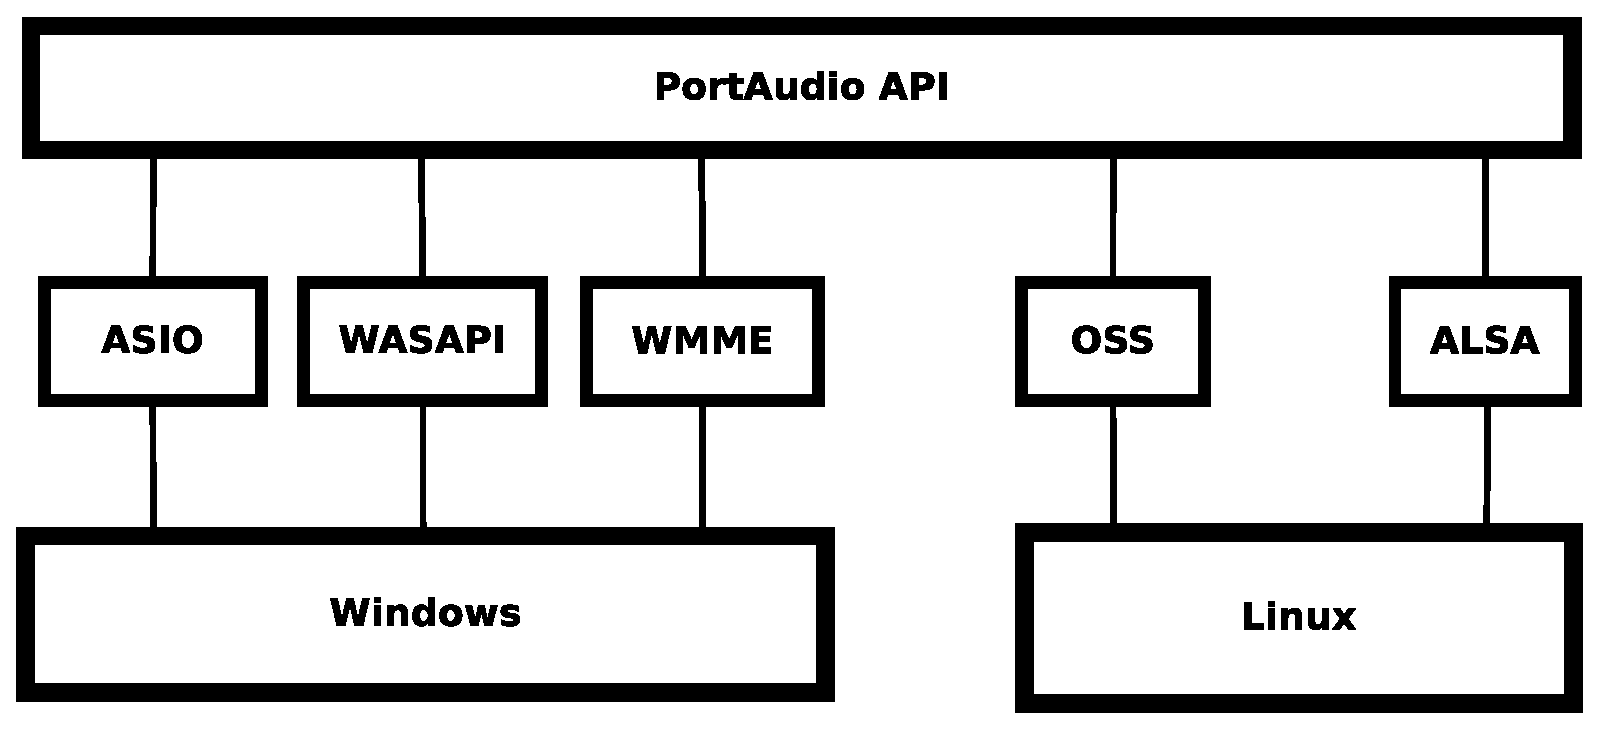
\includegraphics[width=0.75\linewidth]{fig/portaudio}
	\caption{Arquitetura do PortAudio.}
	\vspace{-1cm}
	\caption*{\textbf{Fonte: }Elaborada pelo autor.}
	\label{fig:portaudio}
	\end{minipage}
\end{figure} 

O PortAudio possui suporte para maioria das APIs nativas de cada sistema
operacional. A grande vantagem de utilizar essa ferramenta é que não é
necessário aprender cada API nativa dos sistemas operacionais. Dessa forma é
possível utilizar o mesmo código em diferentes sistemas operacionais,
facilitando a portabilidade do \textit{software} desenvolvido.

A desvantagem de utilizar o PortAudio é que essa ferramenta não fornece total
suporte para toas as funcionalidades de cada API nativa. Por exemplo, o PortAudio não
fornece conversão de taxa de amostragem se for solicitado uma taxa de amostragem
que não seja suportada pela API de áudio nativa. Outro bom exemplo é que o ASIO
SDK permite apenas que uma aplicação seja executada por vez, dessa forma o
PortAudio, atualmente, não suporta a execução de várias aplicações
simultaneamente~\cite{portaudio}.

\end{section}

\begin{section}{X Window System}

O X Window System, também conhecido como X ou X11, é um sistema de janelas
criados pela MIT. Esse sistema atualmente está na sua décima primeira versão
(por isso é também chamado de X11), publicada em 1987. O X11 também é um
protocolo que funciona no modelo cliente-servidor e é utilizado como padrão para
GUIs (do inglês, \textit{graphical user interface}) em sistemas baseados em UNIX
e Linux. Uma visão geral da arquitetura do X Window System é mostrado na
FIgura~\ref{fig:x11}.

\begin{figure}[!h]
	\centering
	\begin{minipage}[c]{\textwidth}
	\centering
	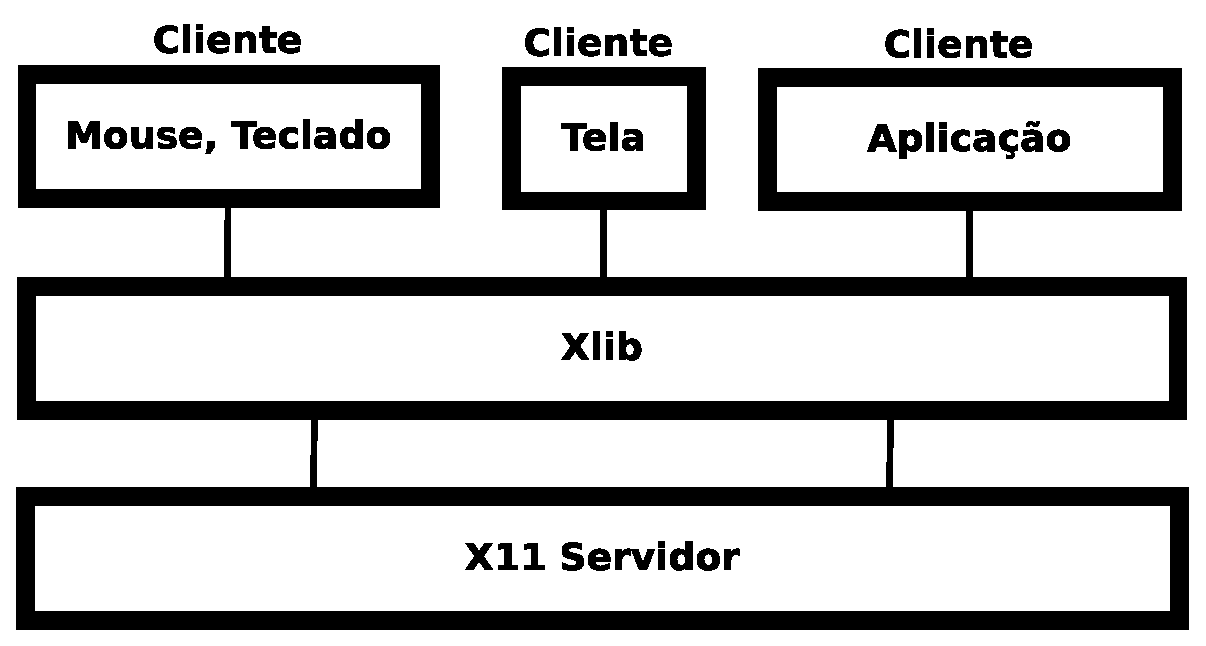
\includegraphics[width=0.6\linewidth]{fig/X11}
	\caption{Arquitetura do modelo cliente-servidor do X11.}
	\vspace{-1cm}
	\caption*{\textbf{Fonte: }Elaborada pelo autor.}
	\label{fig:x11}
	\end{minipage}
\end{figure} 

\vspace{-0.5cm}
O servidor X é executado em computadores com telas de bitmap. O servidor
distribui a entrada do usuário e aceita pedidos de saída de vários programas
cliente através de uma variedade de diferentes canais de comunicação entre
processos~\cite{suse}. É possível criar diversas aplicações utilizando o X11,
como criação de interfaces gráficas para usuários e execução dos movimentos e
eventos de clique do \textit{mouse}. 

As aplicações funcionam como cliente e são desenvolvidas utilizando 
principalmente a API Xlib~\cite{xlib}, uma biblioteca cliente do protocolo X escrita
em C. A Xlib realiza o intermédio entre o cliente (aplicação) e o servidor X.  
\end{section}

\end{chapter}

\begin{chapter}{Protótipo}
O acionador baseado em sopro foi desenvolvido com a intenção de ser
\textit{open-source} e de baixo custo, para que mais pessoas possam ter acesso
a essa ferramenta que pode ser utilizada como método alternativo para o clique
do \textit{mouse}. O circuito do protótipo desenvolvido neste trabalho é mostrado 
na Figura~\ref{fig:circuito}

\begin{figure}[!h]
	\centering
	\begin{minipage}[c]{\textwidth}
	\centering
	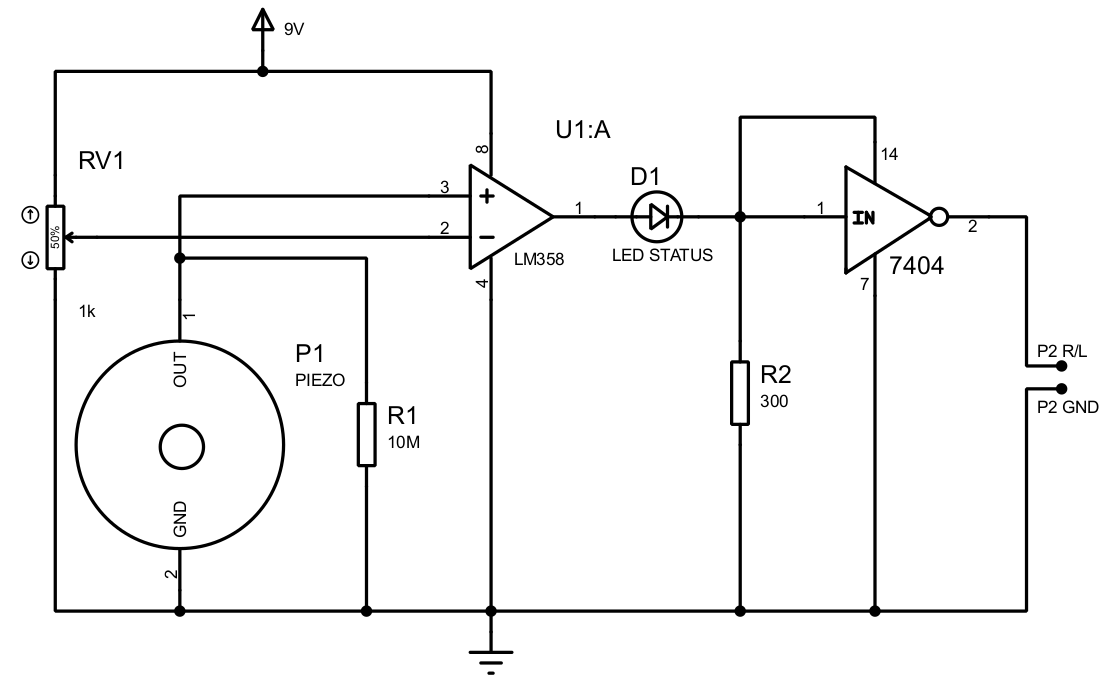
\includegraphics[width=0.9\linewidth]{fig/acionador}
	\caption{Esquemático do acionador baseado em sopro.}
	\label{fig:circuito}
	\end{minipage}
\end{figure} 

O princípio de funcionamento do acionador externo proposto é relativamente
simples. A percepção do sopro é realizada graças ao piezo encapsulado em um
disco redondo que fica acoplado na parte superior do dispositivo. Quando o
usuário realiza o sopro diretamente no piezo, há um estresse mecânico que produz
uma diferença de potencial elétrica nas extremidades do material piezoelétrico. 
Através dessa tensão produzida no piezo, é possível gerar um evento de
clique de \textit{mouse} no computador. O resistor colocado em paralelo com o
piezo é responsável por determinar a sensibilidade com que o transdutor gera
tensão após ser submetido a algum tipo de estresse mecânico. Portanto, quanto
maior o valor de resistência do resistor, maior será a sensibilidade do piezo.
No protótipo desenvolvido, utilizou-se um resistor de 10~M\si{\ohm}, o que
proporcionou uma boa sensibilidade no piezo. Resistores com valores de
resistência maiores que 10~M\si{\ohm}, como 15~M\si{\ohm}, 20~M\si{\ohm} e
30~M\si{\ohm}, também foram testados, contudo a sensibilidade com resistências
maiores que 15~M\si{\ohm} deixava o transdutor muito suscetível a detectar
estresses mecânicos com intensidades não desejadas. Já a
resistência de 
15~M\si{\ohm} não apresentou diferenças significativas na sensibilidade do piezo 
em relação ao resistor de 10~M\si{\ohm}, portanto, a resistêcia de 10~M\si{\ohm}
foi escolhida. 

O sinal da tensão gerado nas extremidades do material piezoelétrico é analógico.
Contudo, como o clique do \textit{mouse} possui uma natureza binária, pois há
apenas dois estados possíveis (clique ativado e clique não ativado), não
seria possível utilizar diretamente essa tensão produzida como forma de ativação
do clique devido a grande quantidade de ruído que esse sinal possui. Por isso 
houve a necessidade de digitalizar a saída do acionador.

A solução encontrada para realizar a tarefa de ``converter'' o sinal analógico
do acionador para um sinal digital, foi a utilização de um amplificador
operacional LM358. Esse componente eletrônico possui a função de comparar duas
tensões que determinam a saída do acionador. Há uma tensão de referência, que
pode ser variável graças a um potenciômetro de 10~k\si{\ohm}, e a tensão
produzida pelo transdutor piezo. O amplificador operacional atua, neste caso,
como um comparador de tensões na configuração não inversora. Quando a tensão de
referência é superior a tensão do piezo, a saída do amplificador é de nível
lógico baixo. Contudo, quando a tensão de referência é inferior a tensão do
piezo, a saída do amplificador é de nível lógico alto. Não há possibilidade da
saída do amplificador ser diferente desses dois casos. Dessa forma, a leitura do
sinal de tensão produzido pelo sopro, com o auxílio do piezo, é binária, o que
ajuda a implementar a emulação dos eventos de clique. É importante ressaltar
que, como o valor de referência pode ser ajustável, graças ao potenciômetro,
esse componente também atua como um ferramenta de ajuste de sensibilidade. Sendo
assim, a intensidade do sopro necessária para que a saída do amplificador seja
de nível lógico alto, configurando assim um clique, pode ser determinada pela
tensão de referência ajustada pelo potenciômetro.

Como um dos objetivos do acionador é ser de baixo custo, a comunicação entre o
acionador desenvolvido e o computador é realizada através da interface de áudio
P2 Jack. Para gerar um pulso na interface de áudio, basta curto-circuitar o pino
de GND com o \textit{Right} e \textit{Left} do P2 Jack do acionador. Para fazer
isso, foi necessário a utilização de uma porta lógica inversora do componente
SN7404, ilustrado na Figura~\ref{fig:sn7404}. Essa porta lógica captura o sinal
da saída do LM358 somente quando a saída do amplificador é de nível lógico alto,
pois a saída desse componente também é utilizado como alimentação do SN7404.
Portanto, quando a saída do amplificador é de nível lógico baixo, o inversor não
funciona, pois não há tensão suficiente para alimentar esse componente. Quando a
saída do LM358 é de nível lógico alto, o inversor é alimentado com uma tensão
suficiente para realizar o funcionamento correto. Essa tensão é utilizada como
entrada do SN7404 que inverte o sinal de entrada para nível lógico baixo. A
saída do inversor é conectada nos pinos  \textit{Right} e \textit{Left} do P2
Jack --- que estão curto circuitados --- gerando um pulso na entrada da
interface de áudio do computador. A partir desse pulso reconhecido pelo
computador é possível realizar a implementação da emulação dos evento de clique
do \textit{mouse}.

\begin{figure}[!h]
	\centering
	\begin{minipage}[c]{\textwidth}
	\centering
	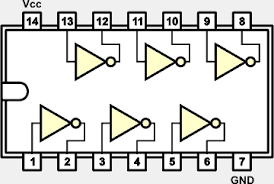
\includegraphics[width=0.45\linewidth]{fig/sn7404}
	\caption{Circuito interno do componente sn7404.}
	\label{fig:sn7404}
	\end{minipage}
\end{figure} 

É importante ressaltar que a tensão de saída do amplificador operacional, quando
está em nível lógico alto, é bem próximo de 9~V. Essa tensão é superior a tensão
recomendada (5,5~V) pela fabricante do componente~\cite{7404}.  Para diminuir
essa tensão para a recomendada, foi utilizado um LED vermelho em série com um
resistor de 300~\si{\ohm}. Quando a saída do amplificador é de nível lógico
alto, há uma queda de tensão do cátodo do LED que é suficiente para alimentar o
inversor. Sendo assim, além de ser utilizado como divisor de tensão, o LED
também funciona como um \textit{feedback} visual, indicando quando o acionador
foi ativado pelo sopro do usuário.  


\begin{section}{Confecção da Placa de Circuito Impresso}

Para a construção da placa do acionador baseado em sopro, o \textit{software}
KiCad foi utilizado como ferramenta para desenvolver o \textit{layout} do
circuito do acionador. Todo o projeto da construção do acionador proposto está
disponível em~\cite{ErickGit} para que qualquer pessoa possa acessar o projeto
e, se desejar, construir seu próprio acionador. É importante ressaltar que
alguns componentes, como o piezo, não possuíam biblioteca nativa no Kicad. Por
isso foi necessário desenvolver uma biblioteca para cada um desses componentes.

Após a construção do \textit{layout} do circuito no Kicad etapa de confecção da
placa foi iniciada. A técnica de transferência térmica, um método bem primitivo,
porém bastante prático e barato, foi utilizada. O circuito é impresso em papel
fotográfico em uma impressora a \textit{laser} na melhor qualidade possível. Em
seguida, o circuito é transferido para uma placa de fenolite ou de fibra de
vidro através de um processo térmico, onde a placa é pressionada por uma
superfície em temperatura relativamente alta. No caso do protótipo construído
neste trabalho, um ferro de passar roupa foi utilizado para realizar esse
processo térmico. É importante pressionar bastante o ferro de passar roupa
contra a placa e realizar movimentos em todas as direções a fim de transferir
totalmente o \textit{layout} do circuito desenhado para a placa. Após o processo
térmico, se algum trecho do circuito não for transferido para a placa, é
possível corrigir, com um pincel marcador permanente de CD/DVD, as trilhas não
transferidas do circuito. 

O processo seguinte a transferência do circuito para a placa é a sua corrosão.
Para isso, é utilizada uma solução de percloreto de ferro. Essa solução é
muito fácil de ser encontrada, pois muitas lojas de eletrônica vendem esse
produto. Geralmente, o percloreto de ferro é vendido em pó, porém é necessário
apenas misturar o produto com água para obter a solução desejada. A placa com o
circuito recém transferido é mergulhada nessa solução e todo o cobre da placa é
corroído, restando apenas o \textit{layout} do circuito desejado. Apos a
corrosão realiza-se a limpeza do circuito com uma água corrente e detergente a
fim de retirar todas as impurezas do circuito. A etapa final consiste em furar a
placa nos locais desejados e realizar a soldagem dos componentes da placa.

\begin{figure}[!h]
	\centering
	\begin{minipage}[c]{\textwidth}
	\centering
	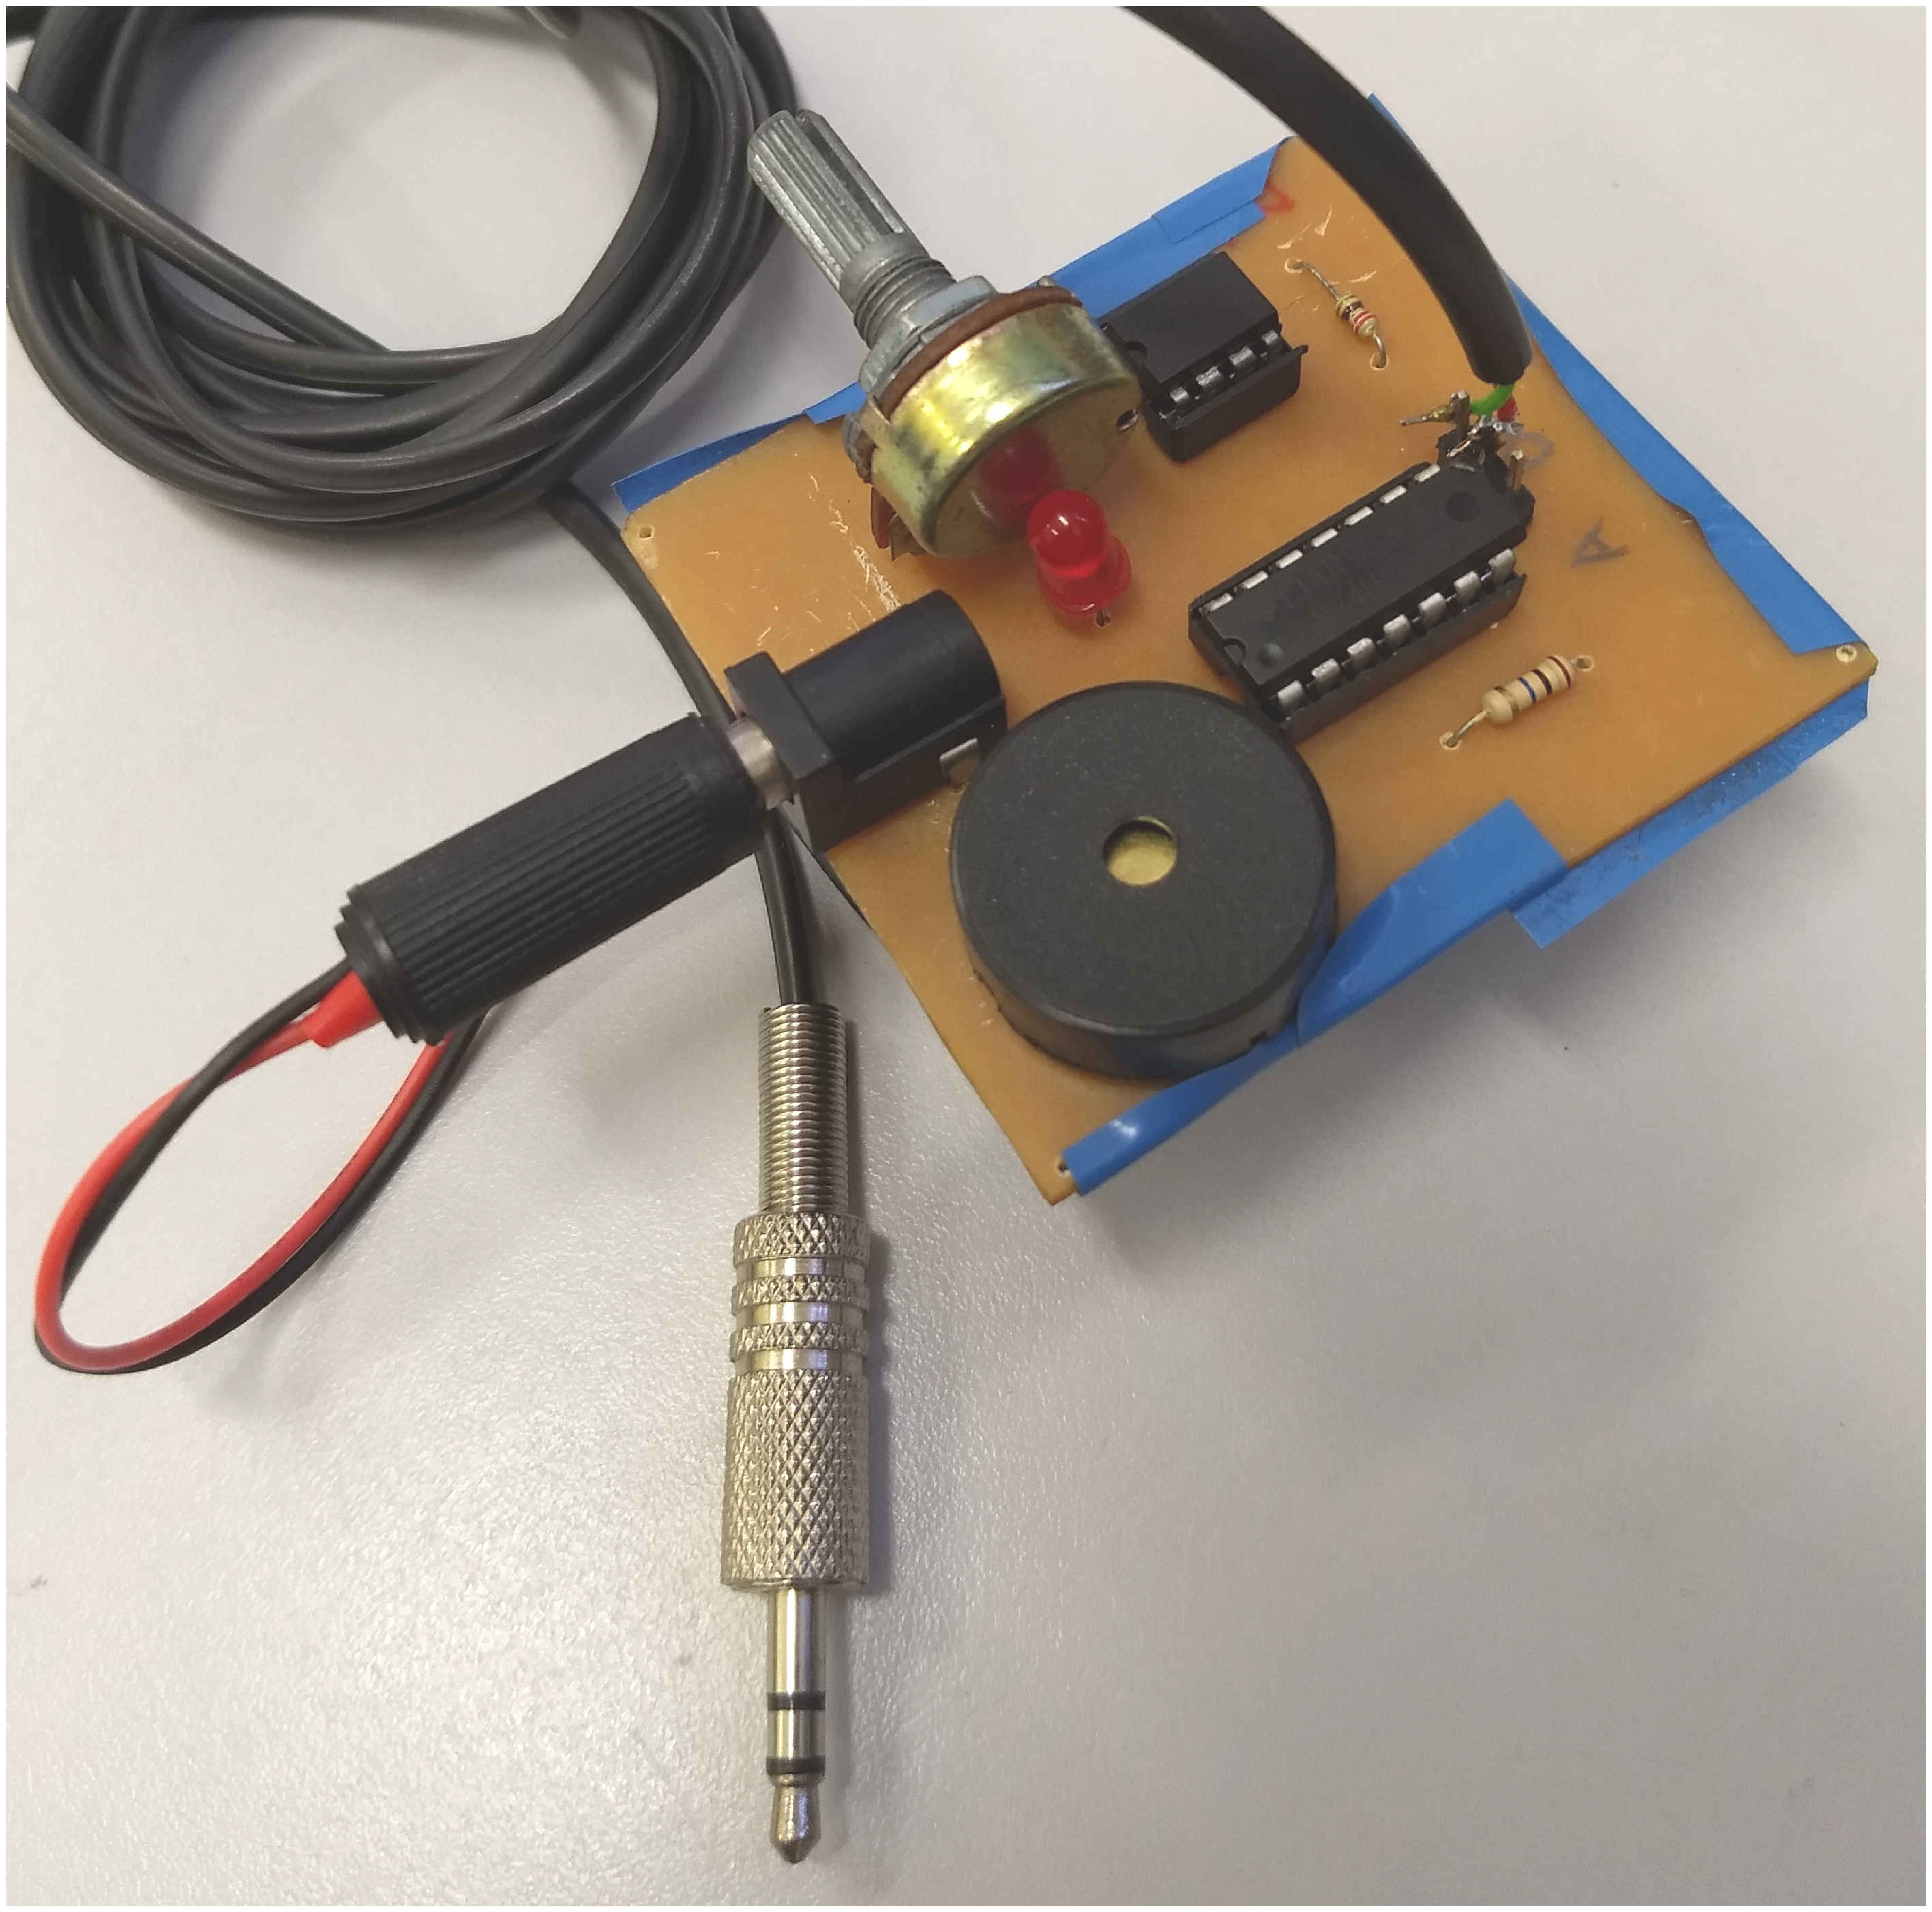
\includegraphics[width=0.45\linewidth]{fig/puff2}
	\caption{Placa de circuito impresso construído como acionador baseado em sopro.}
	\label{fig:placa}
	\end{minipage}
\end{figure} 

A Figura~\ref{fig:placa} mostra a placa confeccionada neste trabalho. É possível
notar que o dispositivo é relativamente pequeno: mede cerca de 7$\times$7
centímetros. Os componentes mais caros utilizados para o desenvolvimento do
acionador externo baseado em sopro foram o disco piezoelétrico, o amplificador
operacional LM358, o inversor SN7404 e a placa de fenolite. 

Cerca de R\$ 30 reais
foram gastos para na protótipo proposto neste trabalho. Esse valor é bem mais
barato que outros acionadores que utilizam o sopro como método não-convencional
para o clique \textit{mouse}, como~\cite{SipPuff}. Os preços tomados como
parâmetro neste trabalho foi baseado na loja Tip
Eletrônica\footnote{\url{http://tipeletronica.com.br/}}. 

\end{section}


\begin{section}{Suporte de Sustentação do Acionador}

O maior desafio encontrado no desenvolvimento deste trabalho foi de encontrar
uma forma que o usuário conseguisse realizar o sopro diretamente no piezo. Os
acionadores baseados em sopro disponíveis no mercado utilizam soluções com tubos
de PVC, onde a pessoa sopra através desse tubo para conseguir utilizar o
acionador. Todavia, esse tipo de solução restringe demais a possibilidade de
mais de uma pessoa utilizar a mesma ferramenta, pois para utilizar esse tipo de
ferramenta, é necessário manter contato direto da boca com o tubo, e isso não é
recomendado devido as questões de higiene pessoal e prevenção de doenças que
podem ser transmitidas pela saliva~\cite{Li2000}.

Algumas soluções, como em~\cite{CorpPuff}, utilizam uma espécie de 
\textit{headset} para sustentar os tubos de PVC próximos a boca do usuário. Isso
serviu como base para a construção do suporte de sustentação desenvolvido neste
trabalho. Inicialmente, a ideia era desenvolver uma ferramenta baseada em
\textit{headsets}, como o mostrado na Figura~\ref{fig:headset}.

\begin{figure}[!h]
	\centering
	\begin{minipage}[c]{\textwidth}
	\centering
	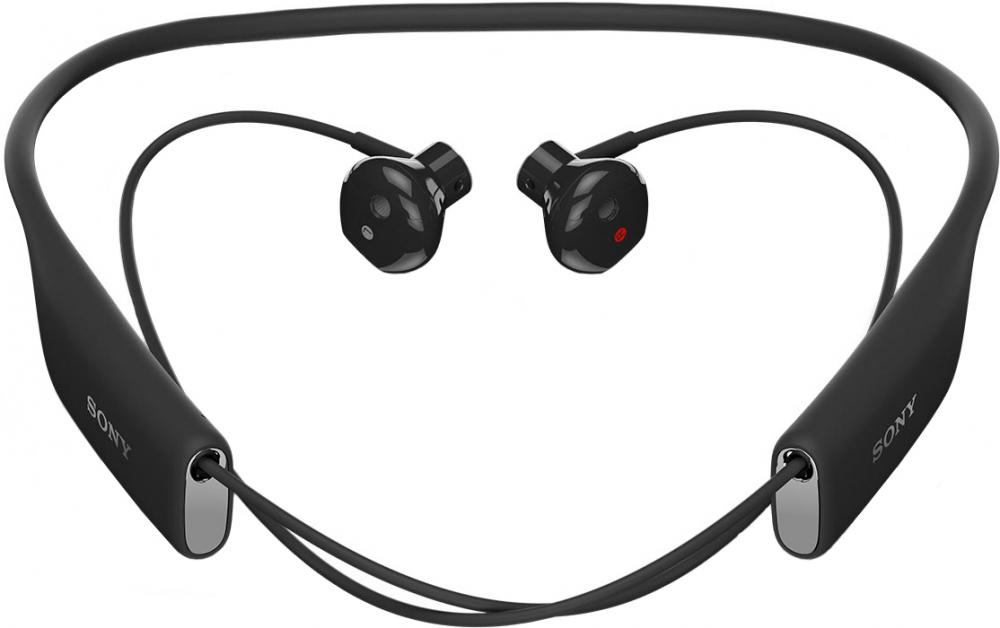
\includegraphics[width=0.3\linewidth]{fig/heaset}
	\caption{Modelo de \textit{headset} inicialmente idealizado.}
	\label{fig:headset}
	\end{minipage}
\end{figure} 

A intenção era desenvolver toda a armação do suporte utilizando arame recozido.
A estrutura ficaria acoplada na parte de trás da cabeça do usuário, se estenderia
pela orelha e as duas extremidades da estrutura seriam responsáveis por segurar
o acionador próximo a boca do usuário. Entretanto, essa solução poderia ser
bastante incômoda, pois o peso do acionador sustentado pela estrutura em volta
da orelha do usuário poderia gerar muito desconforto e insatisfação.

 
\begin{figure}[!h]
	\centering
	\begin{minipage}[c]{\textwidth}
	\centering
	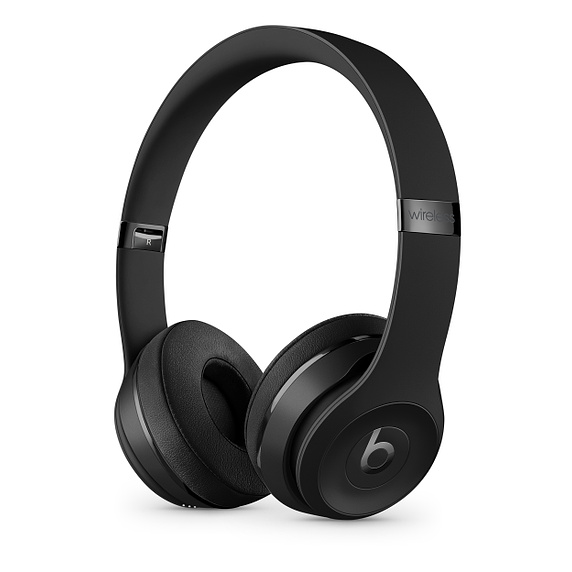
\includegraphics[width=0.35\linewidth]{fig/fone}
	\caption{\textit{Headset} utilizado como base para o suporte de sustentação
do acionador.}
	\label{fig:fone}
	\end{minipage}
\end{figure}


A ideia de utilizar uma ferramenta em forma \textit{headset} não foi totalmente
descartada, dando lugar à ideia de utilizar como base um \textit{headset}
semelhante ao mostrado na Figura~\ref{fig:fone}. 
Essa foi a ideia utilizada para desenvolver o suporte de sustentação do
acionador. Os arames recozidos pensados na solução anterior foram reaproveitados
para a estrutura desenvolvida. A função dos arames é de manter fixo o acionador
próximo a boca do usuário. Os arames foram acoplados nas laterais do
\textit{headset} utilizado e foram curvados de uma forma que as extremidades
dos arames ficassem na frente da boca do usuário. Duas garras do tipo jacaré
foram colocadas nas extremidades  dos arames a fim de acoplar o acionador na
estrutura construída. O resultado do suporte desenvolvido é mostrado na
Figura~\ref{fig:suporte}. 

\begin{figure}[!h]
	\centering
	\begin{minipage}[c]{\textwidth}
	\centering
	\includegraphics[width=0.45\linewidth]{fig/erick}
	\caption{Usuário testando o acionador baseado em sopro em conjunto com o
suporte de sustentação desenvolvido.} %Note que o LED de \textit{status} fica no campo de visão
%do usuário. Sendo assim, o suporte não compromete a visualização do LED que
%informa quando o acionador foi ativado pelo sopro.}
	\label{fig:suporte}
	\end{minipage}
\end{figure}

Com essa estrutura o acionador sempre ficará na frente da boca do usuário,
independentemente da posição da cabeça da pessoa. Além disso, o LED de
\textit{status} fica sempre no campo de visão do usuário. Sendo assim, o suporte
não compromete a visualização do LED que informa quando o acionador foi ativado
ou não pelo sopro. É importante também ressaltar que, como o \textit{headset}
utilizado possui uma estrutura de ajuste de tamanho, o suporte pode ser
utilizado por varias pessoas bastando apenas ajustar o tamanho desejado para
cada tamanho de cabeça. 

\end{section}

\begin{section}{Software}
\textcolor{red}{escrever aqui sobre o software}
\end{section}


\begin{section}{Controle do Cursor do \textit{Mouse}}

O dispositivo baseado em sopro proposto neste trabalho foi desenvolvido para ser
utilizado em conjunto com algum \textit{software} que permite controlar o
ponteiro do \textit{mouse} através de métodos não convencionais. Neste trabalho
não foi desenvolvido nenhum programa que realiza essa função de controle do
cursor. No entanto, foi utilizado o \textit{software} eViacam~\cite{eviacam}.
Esse programa, distrubuído livremente, é multiplataforma e permite controlar os
movimentos do cursor do \textit{mouse} através dos movimentos da cabeça
capturados por uma \textit{webcam}. Além de ser \textit{software} livre e de
código aberto, o motivo principal para a escolha do eViacam foi as suas
configurações que podem ser adaptadas para cada perfil de usuário.

O método de clique habilitado por padrão no eViacam é o \textit{dwell time}. No
entanto, esse método de clique pode ser desabilitado, o que deixa a
possibilidade de utilizar o acionador externo baseado em sopro para realizar a
função de clique. A aba de configuração do clique no eViacam, mostrada na
Figura~\ref{fig:click}, também permote definir o tempo de ativação do clique, no
caso do \textit{dwell time}, que é estabelecido como 10~ds(ou seja, 1 segundo)
como tempo padrão. 

\begin{figure}[!h]
	\centering
	\begin{minipage}[c]{\textwidth}
	\centering
	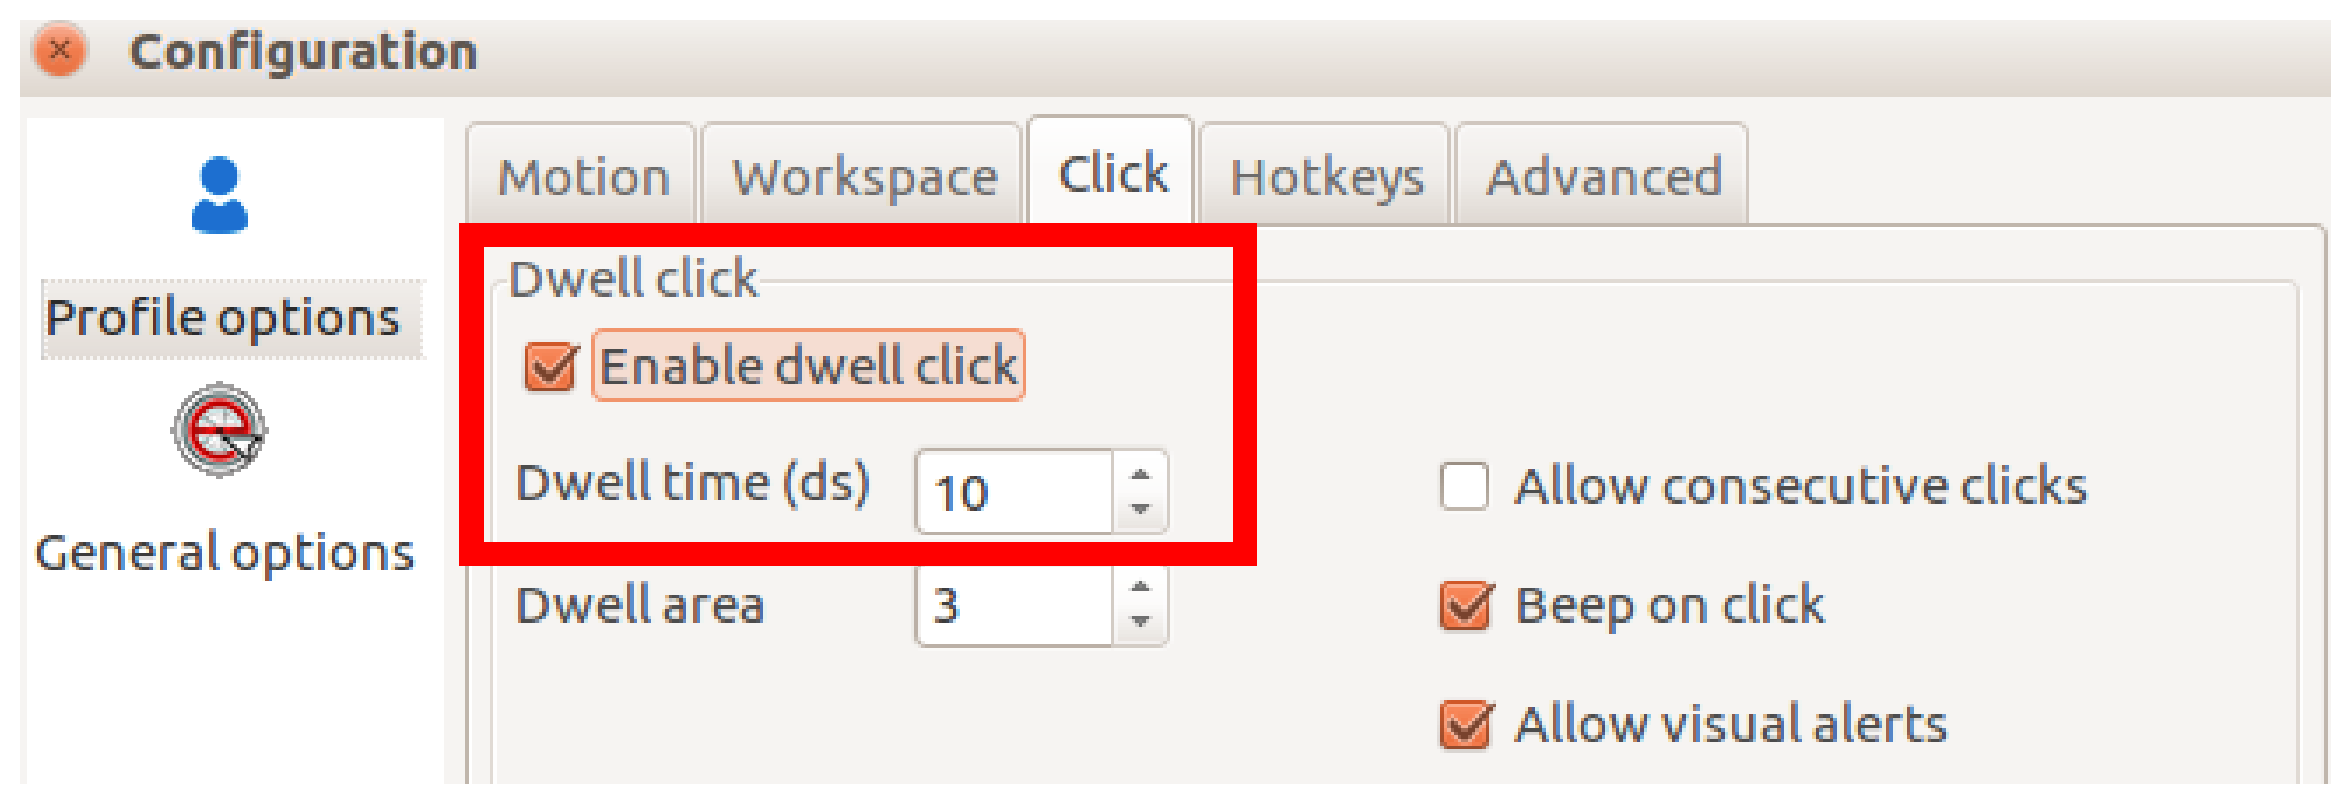
\includegraphics[width=0.7\linewidth]{fig/eviacamclick}
	\caption{Configuração do \textit{dwell time}.}
	\label{fig:click}
	\end{minipage}
\end{figure}
 
Há também a possibilidade de configurar a velocidade de movimentação do cursor
do \textit{mouse}. A Figura~\ref{fig:mouse} mostra, destacado em azul, a
configuração da velocidade do ponteiro nos eixos X e Y. O valor padrão é 10.

\begin{figure}[!h]
	\centering
	\begin{minipage}[c]{\textwidth}
	\centering
	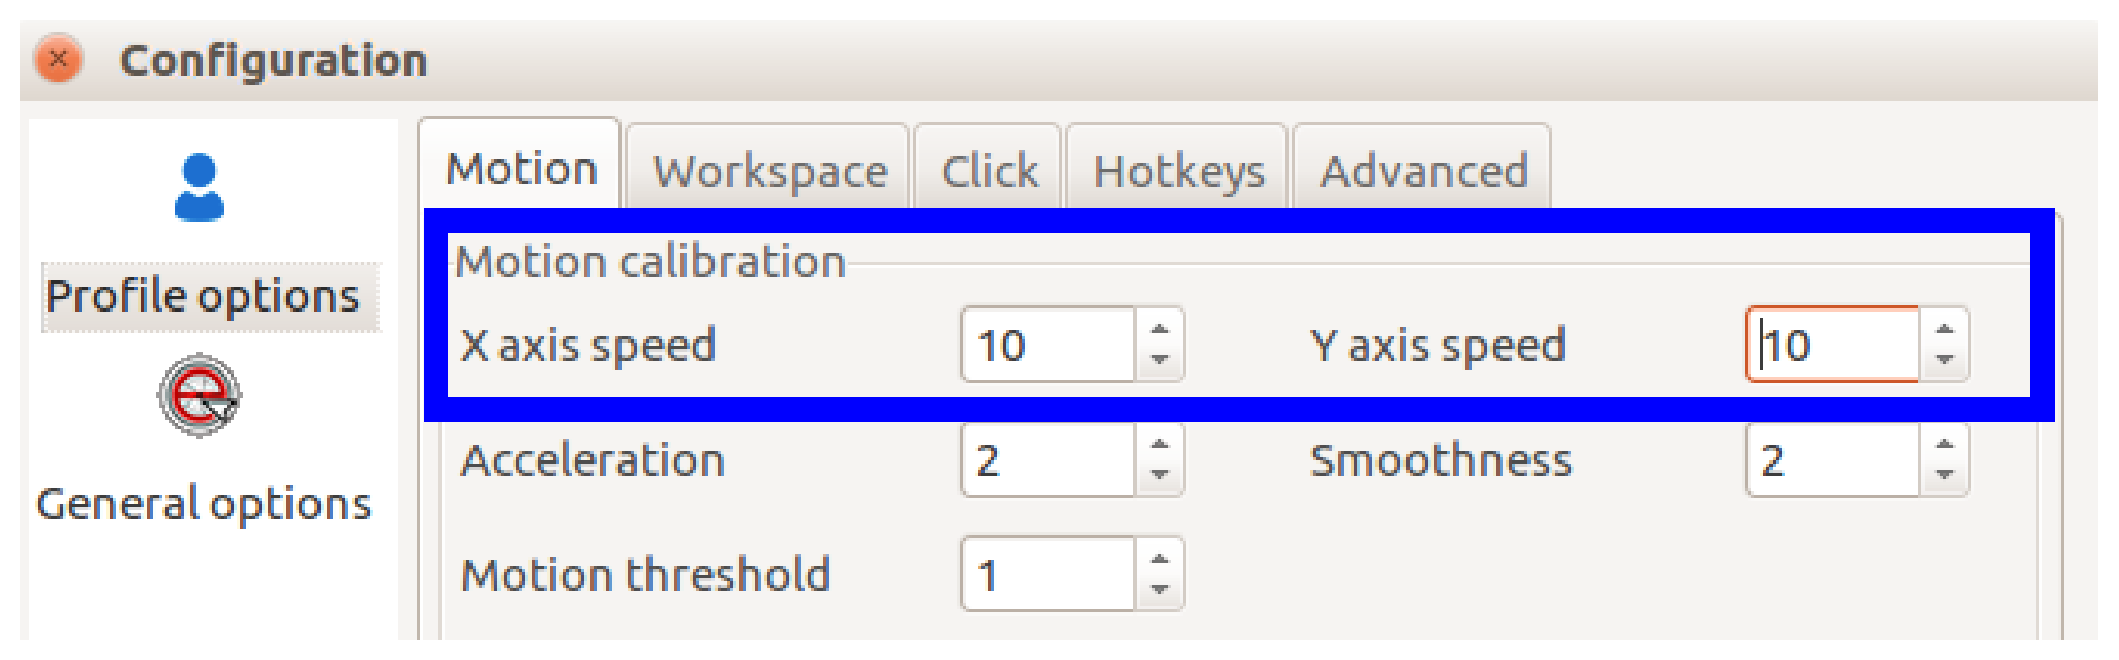
\includegraphics[width=0.7\linewidth]{fig/EviacamConfiguration}
	\caption{Configuração da velocidade de movimento do cursor do \textit{mouse}.}
	\label{fig:mouse}
	\end{minipage}
\end{figure}

\end{section}

\end{chapter}

\begin{chapter}{Testes e Resultados}

Neste capítulo mostra o perfil dos participantes que aceitaram realizar os
testes com o protótipo desenvolvido neste trabalho, bem como o ambiente onde os
testes ocorreram e as tarefas elaboradas para serem realizadas pelos
participantes.  Por último serão apresentados os resultados quantitativos e
qualitativos do teste.  %ok 


\begin{section}{Participantes}

O estudo foi realizado com 7 pessoas do sexo masculino e 3 pessoas do sexo
feminino, totalizando 10 participantes, com idades entre 21 e 28 anos.
Todos os participantes são estudantes de graduação ou pós-graduação da
Universidade Federal do pará (UFPA). O único critério exigido para participar
dos testes era que o participante deveria ter uma certa familiaridade com os
\textit{websites} utilizados nas tarefas.  

A seleção dos voluntários ocorreu através de uma breve conversa com o
participante do experimento, convidando-o a realizar o teste aplicado neste
trabalho. Após a aceitação do participante, o trabalho desenvolvido foi então
apresentado verbalmente, demonstrando a motivação do estudo, todos os objetivos,
a estimativa do tempo de duração do teste e as etapas de cada tarefa que
seria realizada. 
 
Logo após a apresentação do trabalho, o voluntário deveria ler o TCLE (Termo de
Consentimento Livre e Esclarecido), onde foi estabelecido que, ao assinar o
termo, o participante declarava estar ciente de que os dados coletados nos
testes seriam utilizados unicamente para fins de pesquisa acadêmica. Este termo
deixa claro o objetivo do trabalho, informando alguns pontos sobre a restrição
dos dados do participante e declarando por fim que o participante aceitaria os
termos. Após assinar o TCLE, o voluntário estava habilitado a realizar as
tarefas elaboradas. 

\end{section}

\begin{section}{Ambientes de Testes e Procedimentos}

O ambiente onde os testes foram realizados é mostrado na
Figura~\ref{fig:ambiente}.  Como pode ser visto, uma \textit{webcam} foi
posicionada em frente do usuário para capturar os \textit{frames} em tempo real
de seu rosto. O dispositivo de sopro desenvolvido foi fixado próximo a boca do
usuário graças a um \textit{headset} modificado que serviu como suporte de
sustentação que, independentemente da posição da cabeça do usuário, sempre
mantinha o dispositivo de sopro em frente à sua boca.

\begin{figure}[!h]
	\centering
	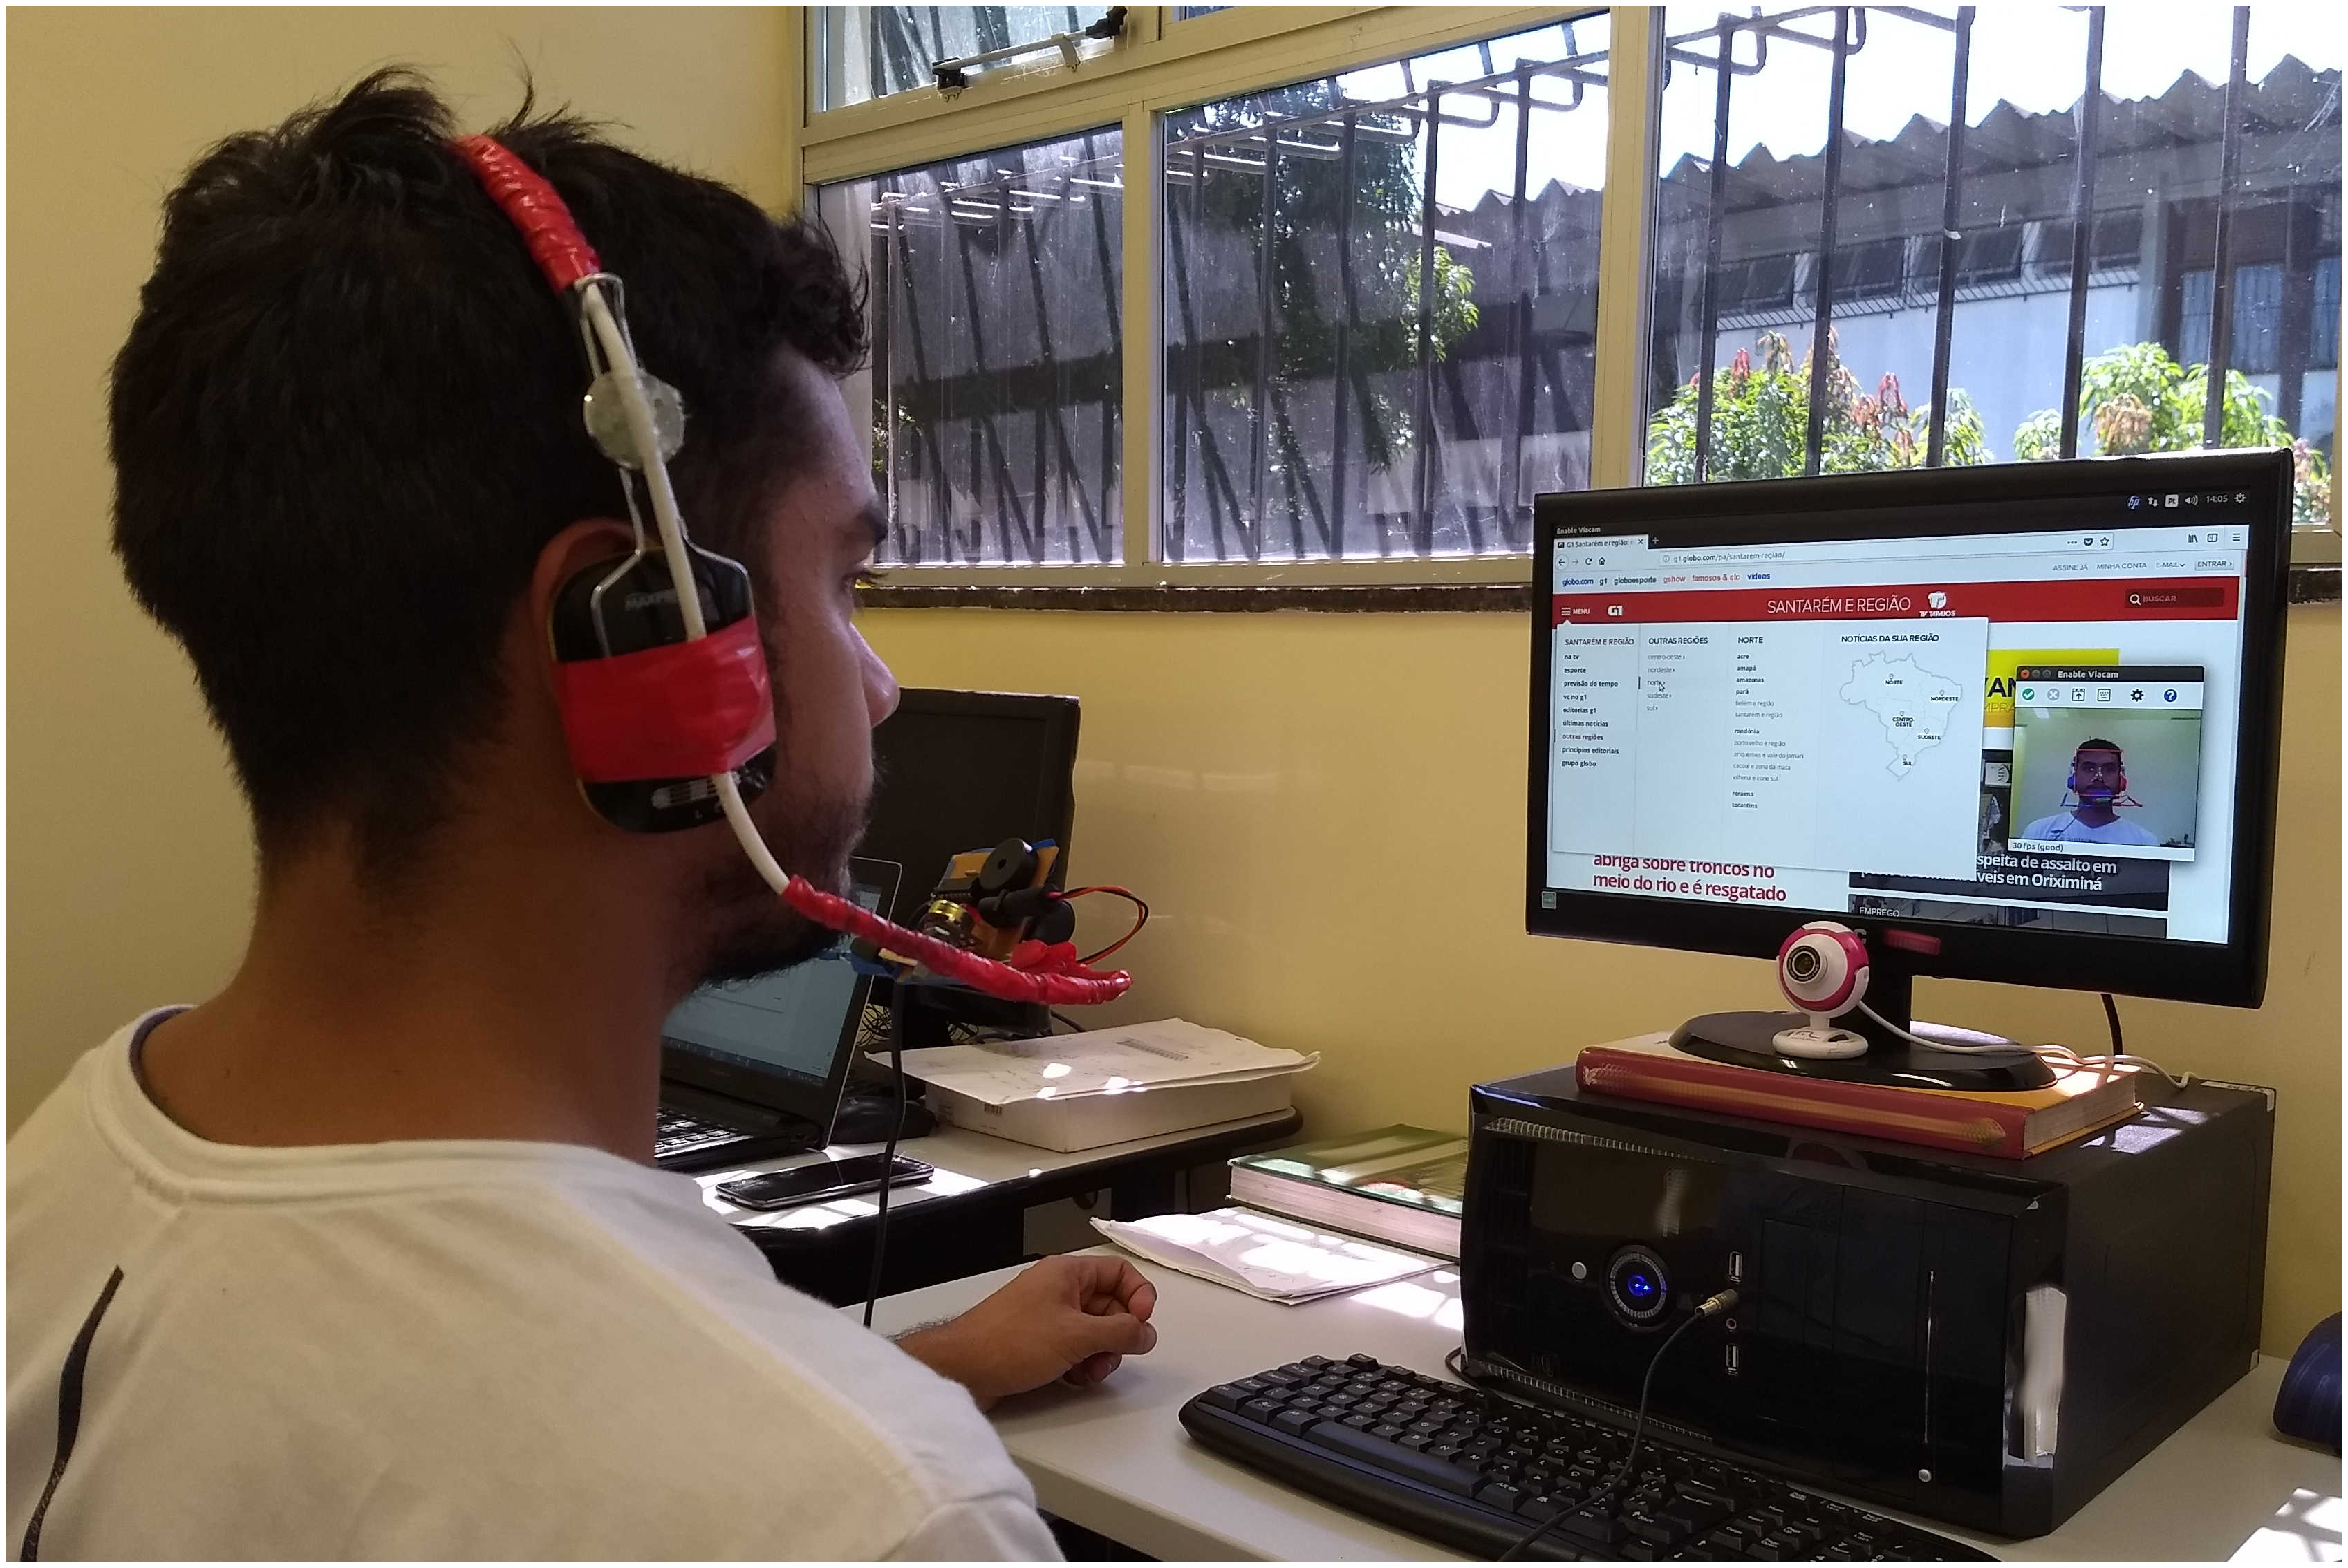
\includegraphics[width=1.00\linewidth]{fig/denes}
	\caption{Um usuário realizando as tarefas no ambiente de teste.}
	\label{fig:ambiente}
\end{figure}

Os testes foram realizados individualmente com todos os participante durante a
luz do dia. Todos estavam devidamente acomodados em uma cadeira com apoio para
a costa. O ambiente estava totalmente iluminado com a luz do sol e também com 
lâmpadas fluorescentes. Os participantes foram questionados se estariam
sentido algum desconforto  no ambiente de teste e todos relataram que
estavam confortáveis. 

O computador utilizado possui um processador Intel Core i5 da 4ª geração,
memória RAM de 4~GB e 1~TB de espaço de armazenamento com o sistema operacional
Ubuntu 16.04 Xenial Xerus x64. O monitor é um AOC E1670SWU de LED com 15,6
polegadas e com resolução de 1366 $\times$ 768.

\begin{figure}[!b]
	\centering
	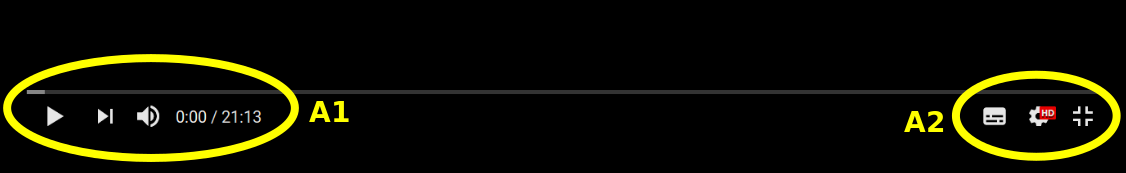
\includegraphics[width=.8\linewidth]{fig/YT}
	\caption{Áreas de interesse do \textit{website} YouTube.}
	\label{fig:youtube}
\end{figure}

\begin{figure}[!b]
	\centering
	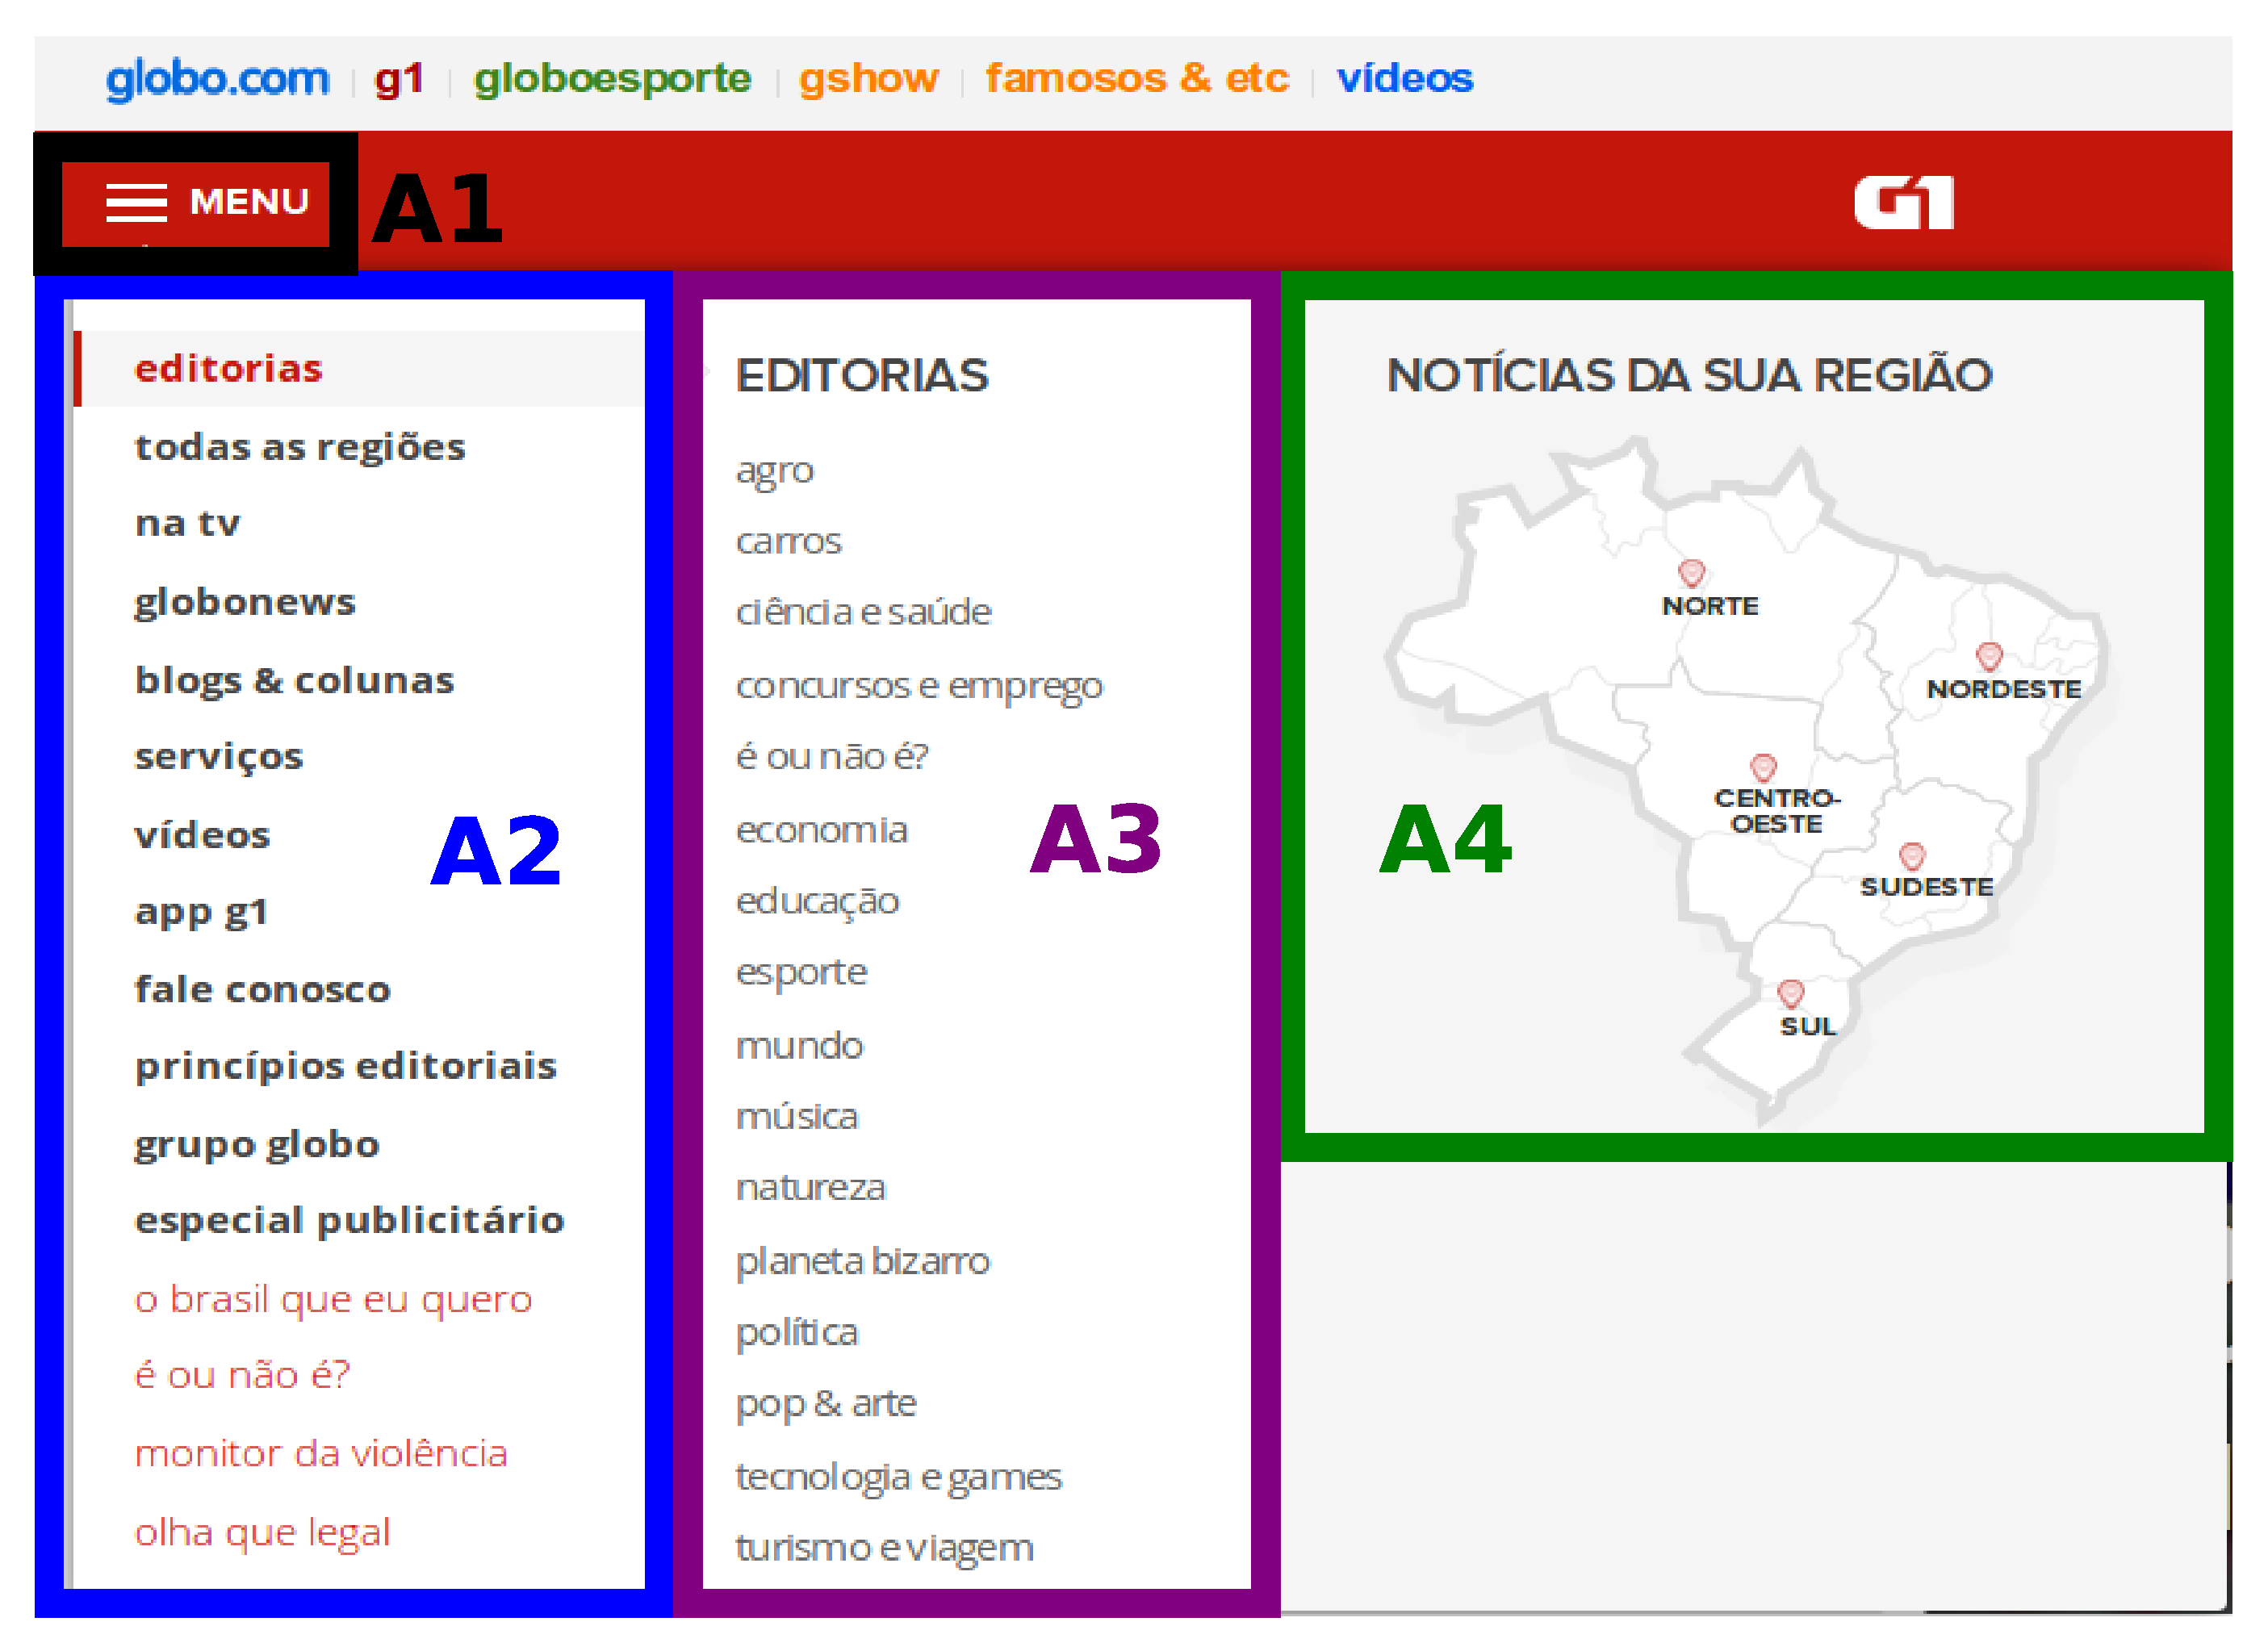
\includegraphics[width=.8\linewidth]{fig/g1}
	\caption{Áreas de interesse do \textit{website} G1.}
	\label{fig:g1}
\end{figure}

As tarefas dos testes foram realizadas nos \textit{websites}
YouTube (\url{https://www.youtube.com/}) e
G1 (\url{https://g1.globo.com/}), mostrados nas
Figuras~\ref{fig:youtube} e~\ref{fig:g1}, respectivamente, com suas respectivas
áreas de interesse destacados em retângulos coloridos e rotulados como A1, A2,
etc. Os \textit{websites} foram escolhidos por não serem totalmente adaptados
para tecnologias alternativas que facilitam a navegação para pessoas com
deficiência. Quando é utilizado o \textit{dwell time} como método de clique, por
exemplo, assistir um vídeo no modo de tela cheia no YouTube torna-se um desafio,
pois o usuário é forçado a mover o cursor do \textit{mouse} a todo o momento
a fim de evitar que cliques involuntários ocorram. Já para o G1, o menu
interativo é um grande problema para aplicações alternativas de controle
do cursor do \textit{mouse}, como o eViacam, visto que os itens na barra de
navegação do menu se expandem e mudam apenas com o simples ato de passar o
ponteiro em cima desses itens (\textit{hover}).

Os testes foram realizados, tanto no YouTube quanto no G1, utilizando o método
baseado em sopro proposto neste trabalho e o \textit{dwell time}. Para controlar
o ponteiro do \textit{mouse}, os participantes utilizaram o \textit{software}
eViacam. Quando os voluntários executaram as tarefas com o protótipo baseado em
sopro desenvolvido neste trabalho, a opção de clique utilizando o 
\textit{dwell time} foi desativada. 

Houve também uma pré-configuração na velocidade de movimentação do cursor do
mouse e também no tempo de clique do \textit{dwell time}. Por meio de testes
exaustivos, verificou-se que a velocidade do cursor do \textit{mouse} que
oferece maior conforto aos usuários ao utilizar o eViacam é 11 em ambos os eixos.
Além disso, o tempo de 15 décimos de segundo (ou seja, 1,5 segundo) para o
clique com o \textit{dwell time} foi estabelecido. O valor padrão no eViacam é
de 10 décimos de segundo, porém foi-se verificado que esse tempo estava
demasiadamente rápido, o que poderia afetar a experiência do usuário.

Os participantes foram instruídos a seguir a mesma rotina de tarefas duas vezes,
utilizando primeiramente o acionador externo proposto neste trabalho e, em
seguida, o \textit{dwell time}. As tarefas mostradas abaixo foram
apresentadas aos usuários com uma breve descrição e em ordem de execução.
Para o G1, a tarefa se iniciou na página principal do \textit{website} enquanto
que para o YouTube, a tarefa se iniciou em um vídeo em modo de tela cheia.  

\begin{itemize}
\item Teste no YouTube (ver Figura~\ref{fig:youtube}):
	\begin{itemize}
	\renewcommand\labelitemi{--}
	\item Clicar no botão de \textit{play} do vídeo.                   \hfill(Área A1)
	\item Clicar no botão de ativar a legenda do vídeo.                \hfill(Área A2)
	\item Diminuir o volume em cerca de 50\%.                          \hfill(Área A1)
	\item Retroceder o vídeo em exebição para os 10 segundos iniciais. \hfill(Área A1)
	\item Clicar no botão de avançar vídeo.                            \hfill(Área A1)
	\item Clicar no botão de sair do modo de tela cheia.               \hfill(Área A2)
	\end{itemize}

\item Teste no G1 (ver Figura~\ref{fig:g1}):
	\begin{itemize}
	\item[$\ast$] Subtarefa 1:
		\begin{itemize}
		\item[--] Mover o cursor para o ícone de menu.        \hfill (Área A1)
		\item[--] Mover para ``editorias''.                   \hfill (Área A2)
		\item[--] Clicar em ``economia''.                     \hfill (Área A3)
		\end{itemize}
	\item[$\ast$] Subtarefa 2:
		\begin{itemize}
		\item[--] Mover o cursor para o ícone de menu.        \hfill (Área A1)
		\item[--] Mover para ``todas as regiões''.            \hfill (Área A2)
		\item[--] mover para ``norte''.                       \hfill (Área A3)
		\item[--] Clicar em ``belém e região''.               \hfill (Área A4)
		\end{itemize}
	\item[$\ast$] Subtarefa 3:
		\begin{itemize}
		\item[--] Mover o cursor até o ícone de menu.         \hfill(Área A1)
		\item[--] Mover para ``todas as regiões''.            \hfill(Área A2)
		\item[--] Clicar no mapa da região norte.             \hfill(Área A4)
		\item[--] Mover para ``pará''.                        \hfill(Área A4)
		\item[--] Clicar em ``santarém e região''             \hfill(Área A4)
		\end{itemize}
	\end{itemize}
\end{itemize}

É importante ressaltar que os voluntários estavam livres para desistir de
qualquer etapa de ambas as tarefas a qualquer momento, porém todos concluíram as
tarefas sem desistir de nenhuma etapa. Cada vez que um participante terminava
uma tarefa, ele era convidado a responder um questionário com seis questões de
múltipla escolha sobre os aspectos do respectivo método de clique utilizado.
Além disso, no final do teste, os usuários responderam uma questão subjetiva
onde eles estavam livres para dar opiniões e sugestões apenas sobre o dispositivo
de sopro utilizado.
\end{section}

\begin{section}{Resultados e Discussão}

O acionador externo baseado em sopro foi comparado, como
método alternativo de clique esquerdo do mouse, com o \textit{dwell time}. Para
isso, foram coletados os dados referentes a: i) tempo gasto para completar cada
tarefa; ii) o número total de cliques executados em comparação com a quantidade
mínima de cliques necessários para executar cada tarefa; iii) a quantidade de
erros de cliques de cada tarefa iv); um questionário de seis perguntas de
múltipla escolha. Por fim, uma pergunta subjetiva foi realizada, onde o usuário
poderia expressar sua opinião acerca do dispositivo desenvolvido neste trabalho.

\begin{subsection}{Tempo de Execução}

A Figura~\ref{fig:tempo} mostra o \textit{boxplot} do tempo de execução de cada
tarefa tanto para o método baseado em sopro quanto para o \textit{dwell time}. A
linha vermelha representa a mediana das distribuições. As ``caixas'',
representadas em linhas azuis, identifica a metade central da distribuição, ou
seja, 25\% dos valores acima da mediana e 25\% abaixo.

\begin{figure}[!h]
	\centering
	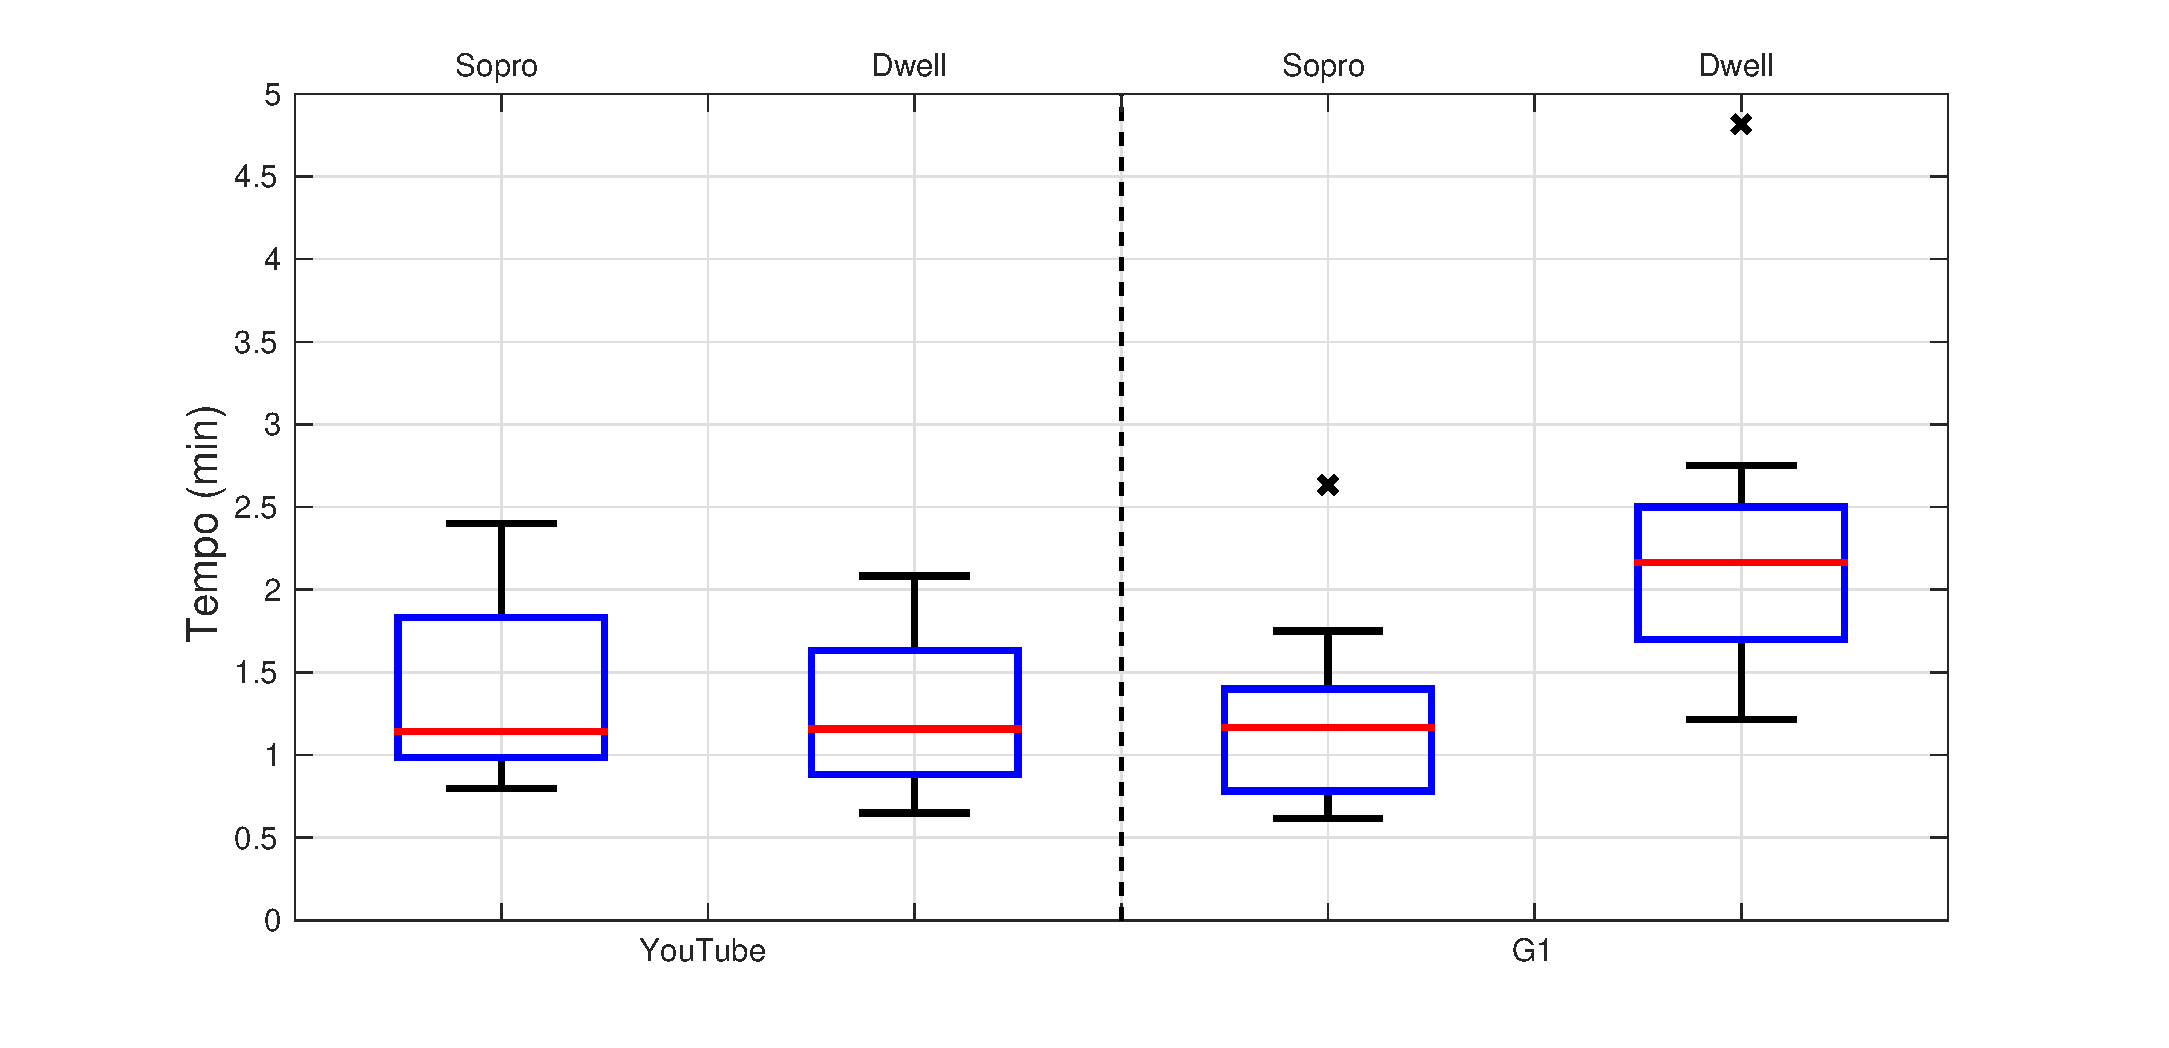
\includegraphics[width=.7\linewidth]{fig/time}
	\caption{Distribuição do tempo de conclusão das tarefas.}
	\label{fig:tempo}
\end{figure}

Analisando a Figura~\ref{fig:tempo}, é possível perceber que, para o YouTube, o
\textit{dwell time} foi o método em que a maioria das pessoas levou menos tempo
para completar a tarefa. Isso pode ser percebido pela amplitude das caixas.
A maioria das pessoas precisou de 50 segundos (50s) a 1 minuto e 40 segundos
(1m40s) para terminar a tarefa do YouTube. Por outro lado, com o dispositivo
baseado em sopro, a maioria das pessoas levou de 1min a 1min50s para concluir a
tarefa.

Já, para o \textit{website} G1, os participantes levaram menos tempo
para finalizar a tarefa utilizando o método de clique baseado em sopro.
A maioria precisou de 45s a 1min30s para terminar a tarefa do G1. Apenas uma
pessoa levou quase 3 minutos para concluir as tarefas do G1, o que explica o
valor de \textit{outlier} exibido como um ``x'' acima da respectiva caixa do
G1. Com o \textit{dwell time}, na tarefa do G1, também houve um caso
\textit{outlier} onde um voluntário completou a tarefa em quase 5 minutos, no
entanto, a maioria dos participantes precisou de 1min45s a 2min30s para terminar
essa tarefa, um tempo superior ao método de clique baseado em sopro.

Como o primeiro método de interação não convencional foi o dispositivo de sopro,
os participantes estavam mais familiarizados quando as tarefas foram executados
pela segunda vez (utilizando o \textit{dwell time}). Isso pode ser observado no
tempo em que os usuários gastaram para executar a tarefa do YouTube, onde o
\textit{dwell time} foi o método alternativo de clique em que  os participantes
levaram menos tempo para concluir a tarefa. No entanto, para o G1, mesmo os
participantes já sabendo exatamente todos os passos do tarefa (pois eles já
tinham executado-a anteriormente com o dispositivo de sopro), o tempo foi maior
com o \textit{dwell time}. Isso aconteceu porque o G1, assim como diversos
outros \textit{websites}, não é adaptado para tecnologias alternativas que usam
o \textit{dwell time} como método de clique, o que dificulta demais a seleção
correta dos itens desejados no menu, especialmente devido a proximidade entre os
itens, os quais são expandidos apenas passando o ponteiro do mouse sobre eles.

\end{subsection}

\begin{subsection}{Quantidade de Cliques}

A Figura~\ref{fig:cliques} mostra a quantidade de erros de clique (cliques
involuntários ou sem sucesso), cometidos pelos usuários em cada tarefa. Alguns
participantes realizaram a tarefa do YouTube usuando o \textit{dwell time} sem
erros de cliques, representado pela caixa em azul a partir do zero, fato que não
aconteceu com a ferramenta baseada em sopro. No entanto, na tarefa do G1, o
número de erros aumentou consideravelmente no \textit{dwell time}, onde a
maioria dos voluntários errou entre 4 a 12 vezes.

\begin{figure}[!h]
	\centering
	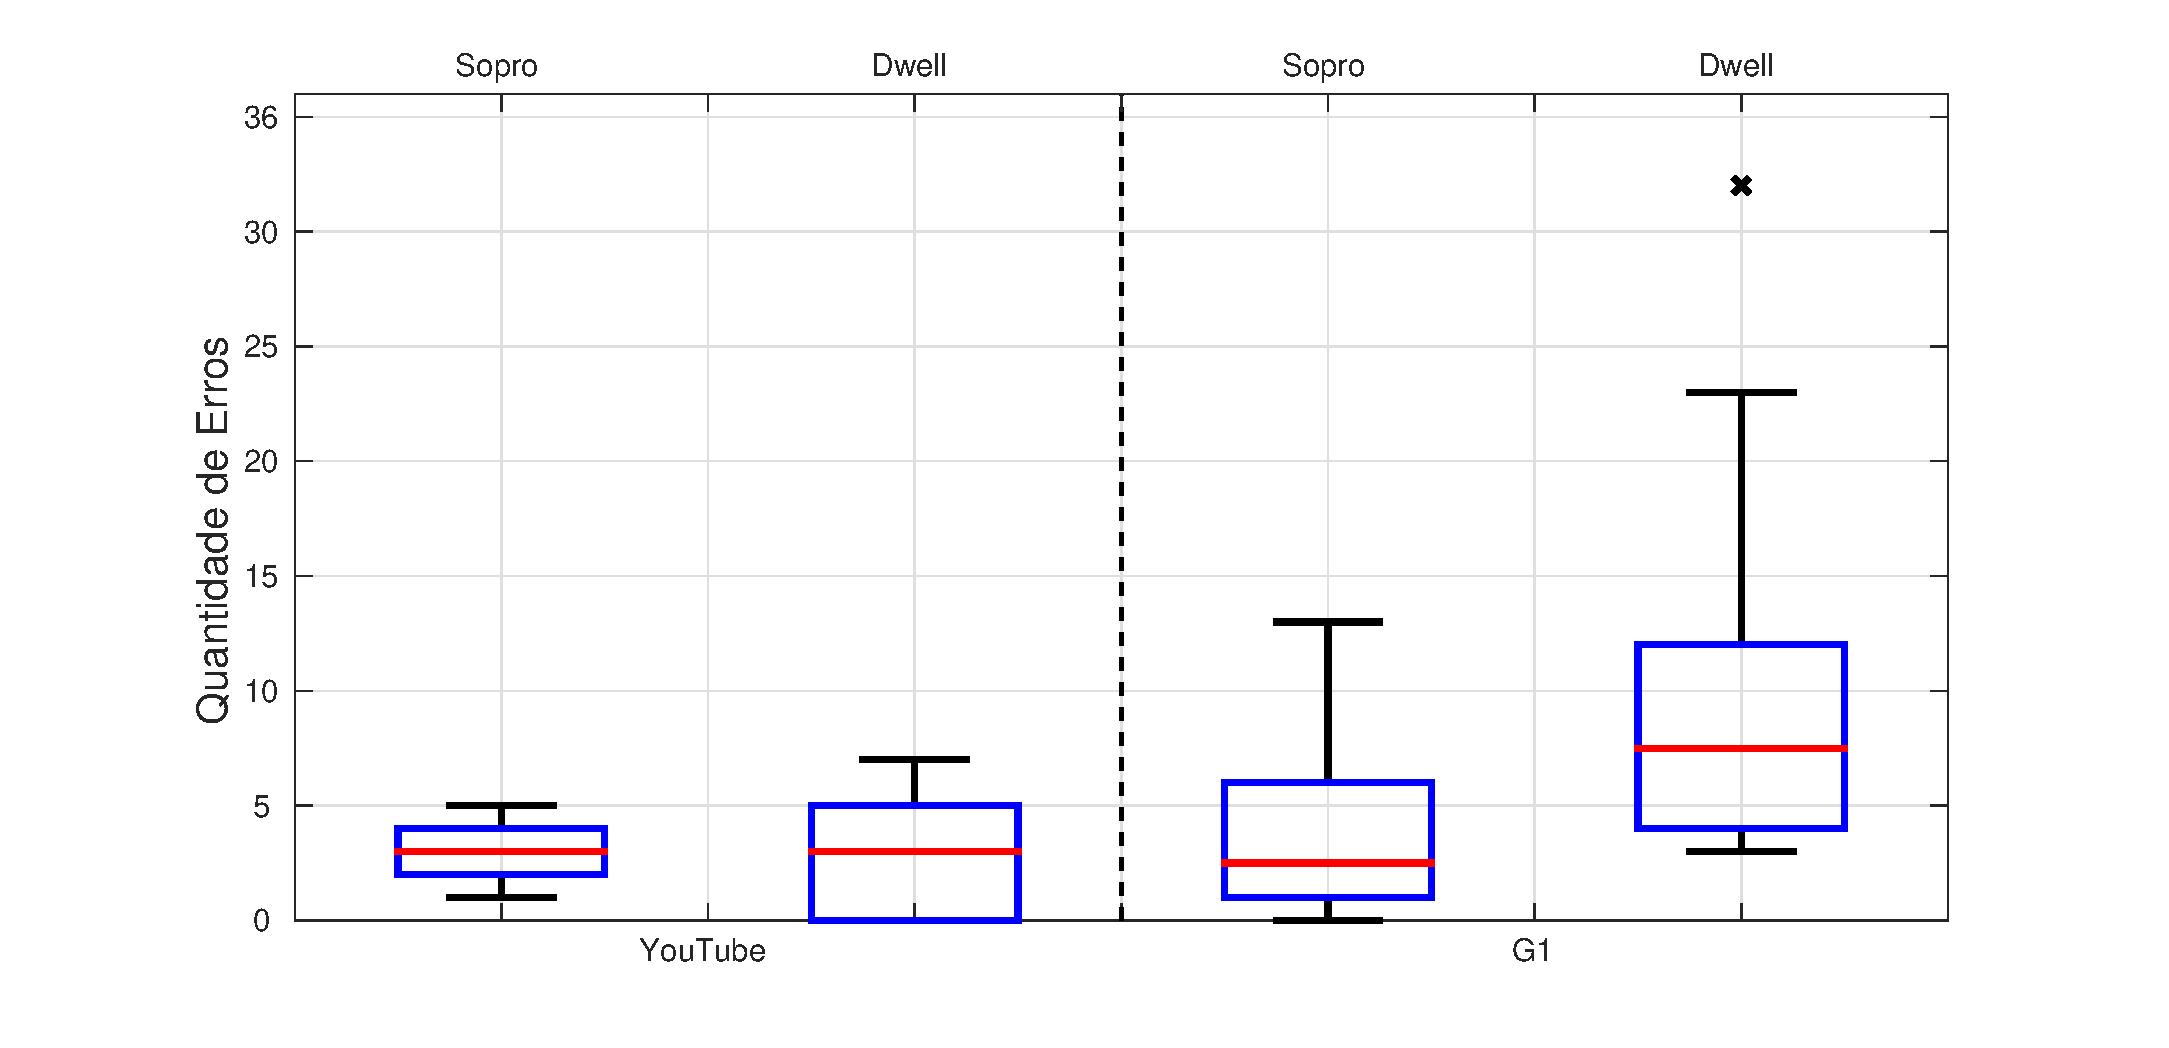
\includegraphics[width=.7\linewidth]{fig/erros}
	\caption{Distribuição da quantidade de erros cometidos em cada tarefa.}
	\label{fig:cliques}
\end{figure}

A maioria dos dos erros de cliques cometidos pelos participantes com o
dispositivo baseado em sopro foi causado por cliques sem sucesso, onde a pessoa
soprava diretamente no transdutor piezoelétrico e o clique não ocorria. Isso
aconteceu principalmente no YouTube, pois essa tarefa foi a primeira a ser
realizada pelos participantes e eles não sabiam ainda exatamente a intensidade
correta de sopro para que o clique ocorresse. Porém, isso não aconteceu com o
\textit{dwell time}, pois a função de clique é ativada depois de um certo
tempo em que o cursor do \textit{mouse} fica sobre uma mesma área. Portanto,
todos os erros cometidos pelos participantes utilizando o \textit{dwell time}
foram causados por cliques involuntários.

As Figuras~\ref{fig:dwellclicks} e~\ref{fig:puffclicks} mostram a quantidade
total de cliques executados pelos usuários utilizando o \textit{dwell time} e o
dispositivo baseado em sopro, respectivamente. A quantidade mínima necessária
para a conclusão das duas tarefas era de seis cliques para a tarefa do YouTube e
quatro cliques para a tarefa do G1. Foram considerados os cliques
realizados corretamente, os cliques involuntários e os
cliques errados (quando o usuário clicava intencionalmente em itens que não
estavam previstos nas tarefas).

É importante notar que eViacam apresentou alguns problemas em detectar a face do
partcipante, e isso afetou diretamente a quantidade de cliques realizados. A
detecção facial falhou diversas vezes quando o participante tentava posicionar o
ponteiro do \textit{mouse} nos cantos da tela. À medida que o cursor se
aproximava dos cantos, a velocidade no movimento do cursor (controlada pelo
rastreador de face do eViacam) diminuía, o que causou muitos cliques
involuntários quando os usuários estavam realizando as tarefas com o
\textit{dwell time}, pois o cursor ficava sobre uma determinada área por
tempo suficiente para que a ação de clique fosse executada.

\begin{figure}[!h]
	\centering
	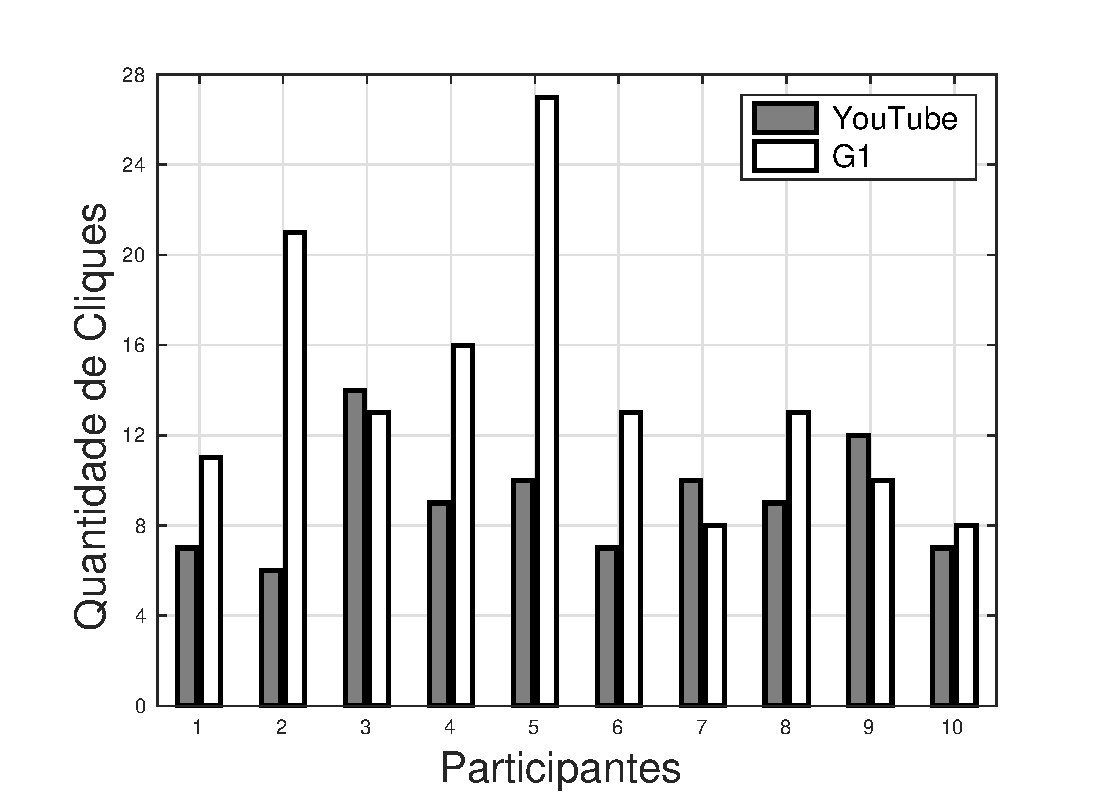
\includegraphics[width=1.00\linewidth]{fig/DwellClicks}
	\caption{Distribuição da quantidade de erros cometidos em cada tarefa.}
	\label{fig:dwellclicks}
\end{figure}

Devido a isso, a quantidade de cliques quando os usuários utilizaram o
\textit{dwell time}, como mostrado na Figura~\ref{fig:dwellclicks}, foi bastante
alta. No total, 90\% dos participantes não conseguiram concluir a tarefa do
YouTube com o valor mínimo de cliques estipulados (seis cliques). A situação
piorou na tarefa o G1, uma vez que nenhum participante conseguiu terminar a
tarefa realizando apenas a quantidade mínima de cliques, resultando em uma média 
bem alta: 14 cliques para uma tarefa que exigia apenas quatro.
  
A quantidade de cliques foi maior na tarefa do G1 devido a precisão
relativamente alta necessária para selecionar os pontos desejados. O voluntário
tentava clicar em ``economia'', mas acabava clicando no item ``educação'' devido
a grande proximidade desses itens localizados no menu do \textit{website}
(ver Figura~\ref{fig:g1}). Isso ocorreu com diversos participantes, que muitas
vezes ficaram frustrados por não conseguir clicar no item desejado.

\begin{figure}[!h]
	\centering
	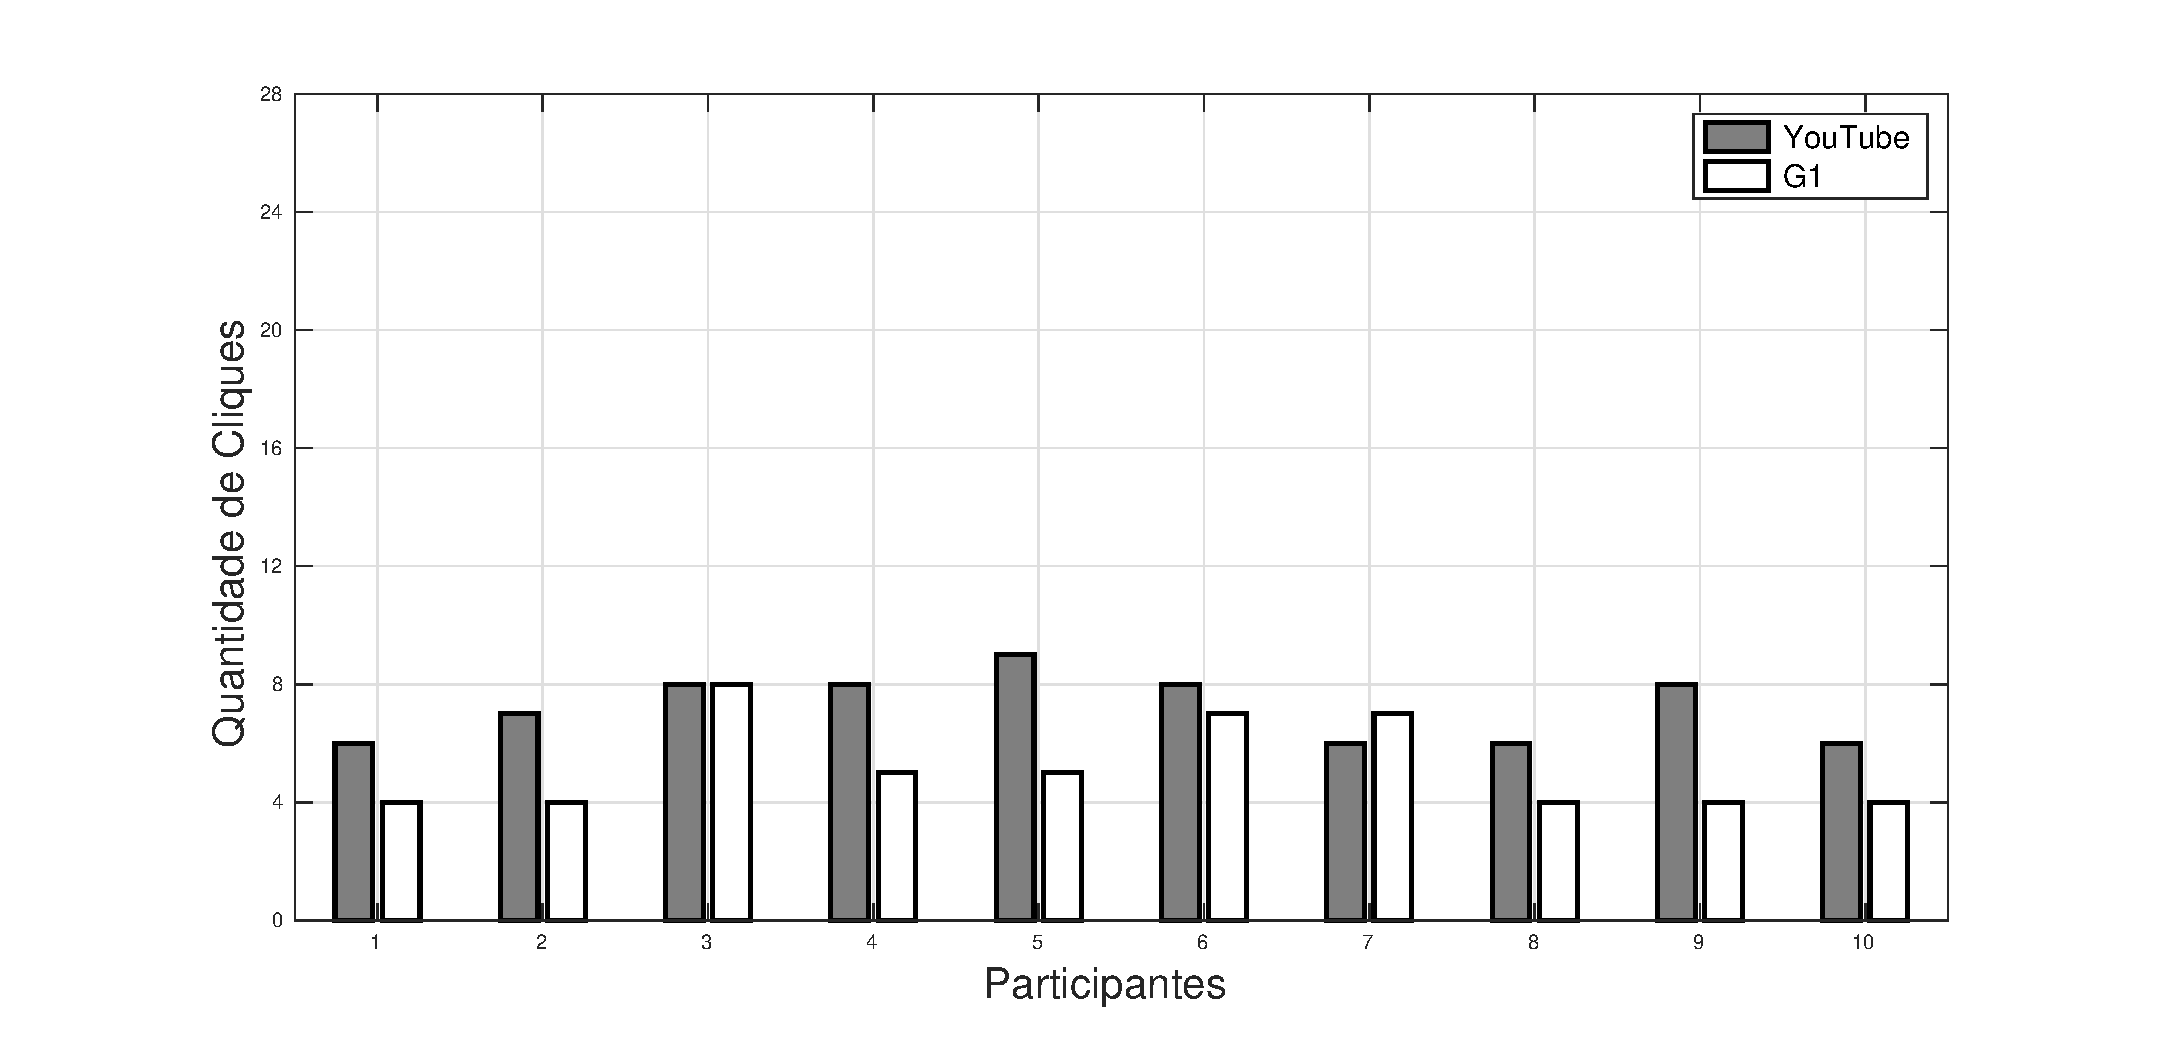
\includegraphics[width=1.00\linewidth]{fig/PuffClicks}
	\caption{Distribuição da quantidade de erros cometidos em cada tarefa.}
	\label{fig:puffclicks}
\end{figure}

No entanto, com o dispositivo baseado em sopro, os participantes realizaram
menos cliques do que com o \textit{dwell time}, como pode ser visto na
Figura~\ref{fig:puffclicks}. Na tarefa do YouTube, por exemplo, quatro pessoas
(os participantes 1, 7, 8 e 10) conseguiram concluir a tarefa utilizando somente
seis cliques. No G1, 50\% das pessoas completaram a tarefa utilizando o número
mínimo de cliques necessários, enquanto que os demais precisaram de oito clique
no máximo.

À primeira vista, quando os participantes utilizaram o protótipo baseado em
sopro, o maior número de cliques ocorreu na tarefa do YouTube. Isso de fato
aconteceu, mas devido ao eViacam, que muitas vezes falhava em detectar o rosto
do participante durante a tentativa de posicionar o cursor nos cantos inferiores
do monitor, como relatado anteriormente.
  
Na tarefa do G1, por outro lado, a dificuldade foi novamente devido as áreas
clicáveis do menu desse \textit{website} estarem muito próximas umas das
outras. No entanto, notou-se que algumas pessoas moviam levemente a cabeça
enquanto sopravam, principalmente devido à força aplicada no peito durante a
expiração do ar. Consequentemente, o cursor do \textit{mouse} também se movia e
esse movimento era suficiente para que o ponteiro se deslocasse para outra
região, fazendo o usuário clicar em um alvo indesejado.
\end{subsection}

\begin{subsection}{Questões de Múltipla Escolha}
A seguir, será mostrado os resultados das seis questões de múltipla escolha 
respondidas pelos voluntários. Essas questões podem ser visualizadas na
Tabela~\ref{tab:quest}.

\begin{table}[!h]
\centering
\small
\def\arraystretch{1.0}
\begin{tabular}{c|ll}
	\hline
	\hline
	 \textbf{Pergunta} &\multicolumn{2}{c}{\textbf{Resposta}} \\
	\hline
	 Como foi sua experiência usando esse método alternativo de clique? & 1 -- insuficiente        & 5 -- excelente   \\
	 O que você achou do tempo para realizar a tarefa?                  & 1 -- lento               & 5 -- rápido      \\
	 Como foi a precisão para realizar a tarefa?                        & 1 -- insuficiente        & 5 -- excelente   \\
	 Como foi o esforço cognitivo para realizar a tarefa?               & 1 -- alto                & 5 -- baixo       \\
	 Como foi o esforço físico para realizar a tarefa?                  & 1 -- alto                & 5 -- baixo       \\
	 Você se concentrou mais na tarefa ou no método de clique?          & 1 -- no método           & 5 -- na tarefa   \\
	%\hline
	%\textbf{\#}& \multicolumn{3}{c}{Based on your experience, what suggestions
	%would you give about the puff-based device?} \\
	\hline
	\hline
\end{tabular}
\caption{Perguntas utilizadas no questionário objetivo.}
\label{tab:quest}
\end{table}

As Figuras~\ref{fig:DwellQuestions} e~\ref{fig:PuffQuestions} mostram uma visão
geral de todas as respostas do questionário de múltipla escolha dadas pelos
participantes. A escala Likert foi utilizada para representar as respostas, que
variam de 1 a 5, tanto para o \textit{dwell time} quanto para o dispositivo
baseado em sopro.  A resposta 1, colorida em vermelho, significa muito ruim,
enquanto que a resposta 5, colorida em verde escuro, significa muito bom. Ao
realizar um rápida comparação entre as respostas, é possível afirmar que os
participantes se sentiram mais satisfeitos com o desempenho geral do dispositivo
de sopro do que com o \textit{dwell time}, pois a maioria das respostas
para o método de clique baseado em sopro, em ambas as tarefas, realizadas foram 4
ou 5, como mostrado na Figura~\ref{fig:PuffQuestions}, enquanto que as respostas
para o \textit{dwell time} variaram de 3 a 5, como mostrado na
Figura~\ref{fig:DwellQuestions}.  

\begin{figure}[!h]
	\centering
	\begin{minipage}[c]{\textwidth}
	\centering
	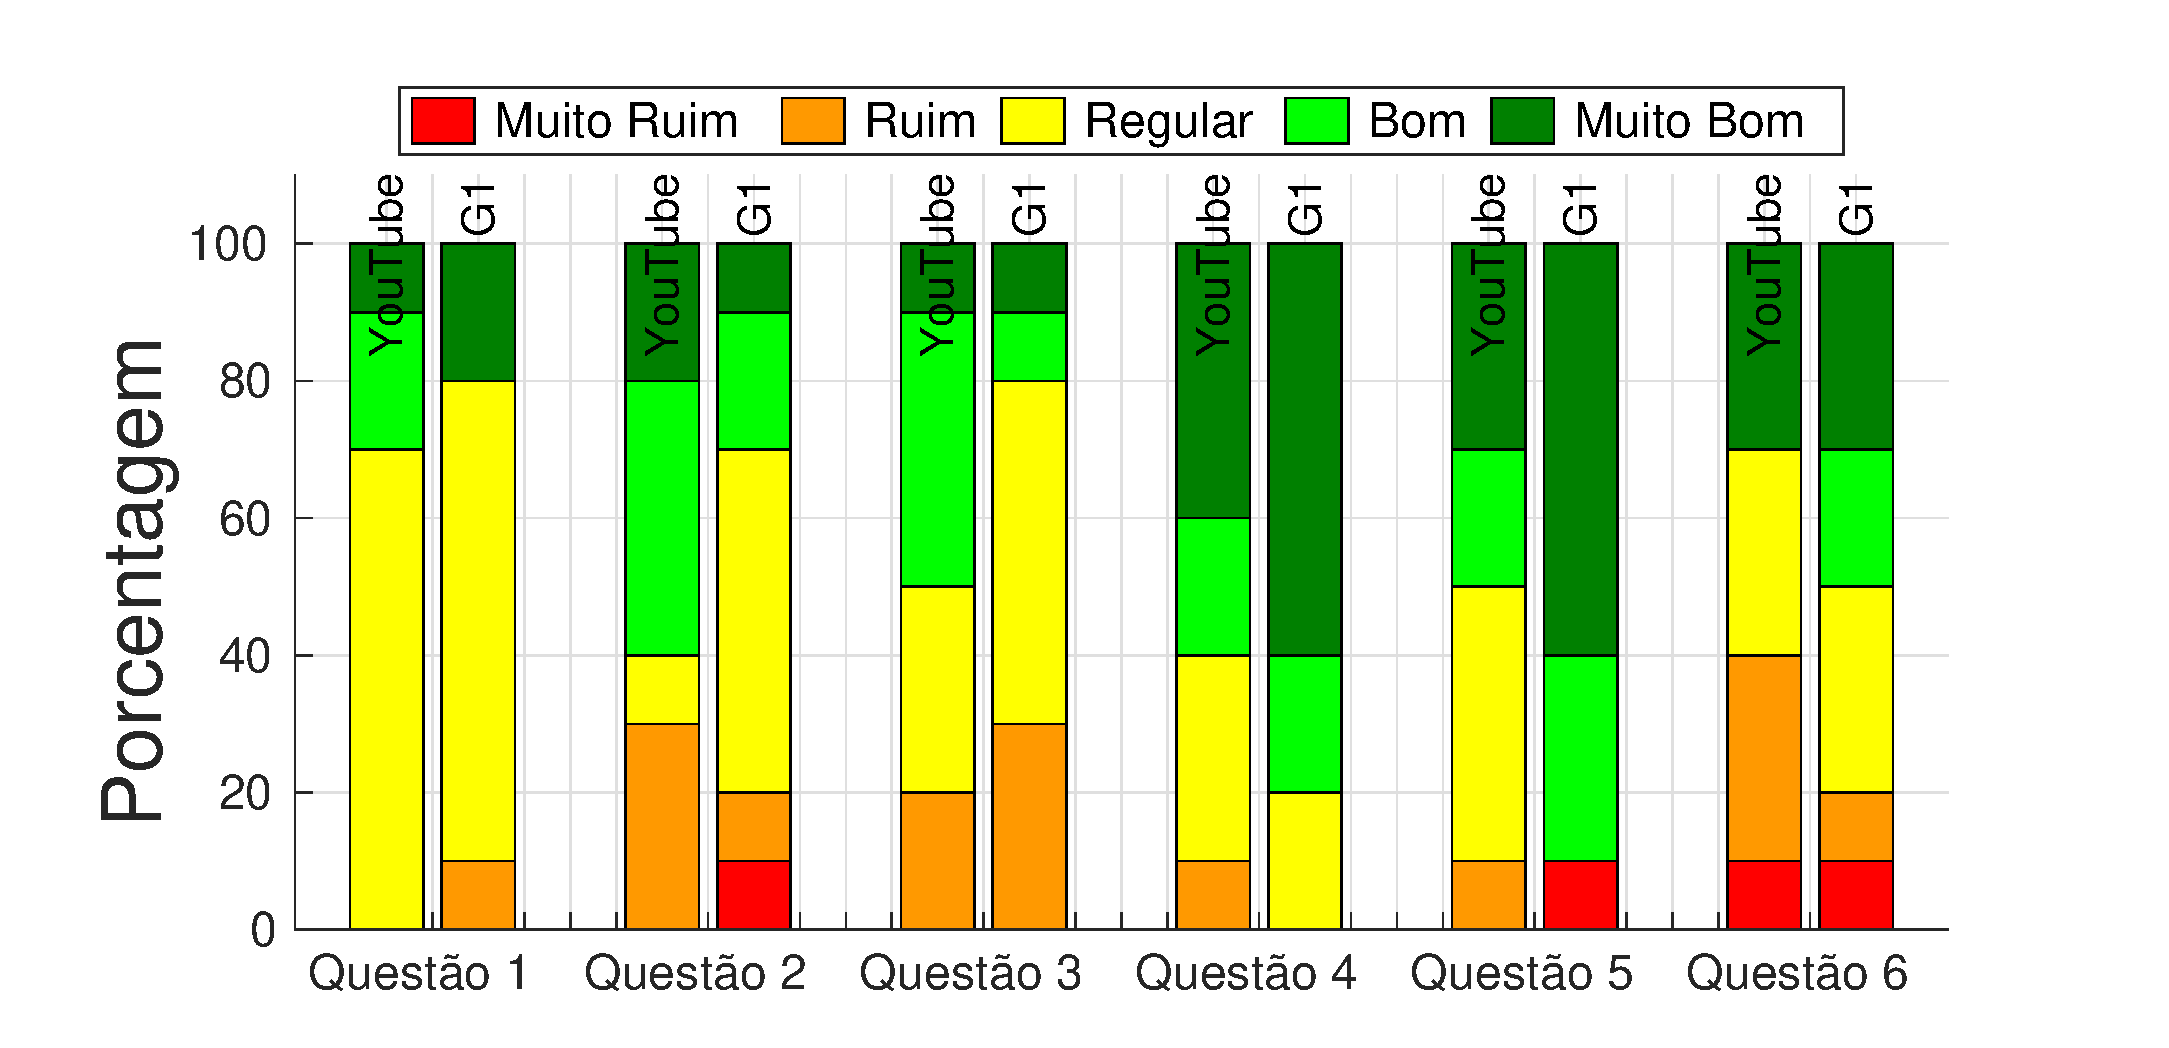
\includegraphics[width=0.9\linewidth]{fig/DwellQuestions}
	\caption{Escala Likert das respostas do \textit{dwell time}.} 
	\label{fig:DwellQuestions}
	\end{minipage}
\end{figure}

\begin{figure}[!h]
	\centering
	\begin{minipage}[c]{\textwidth}
	\centering
	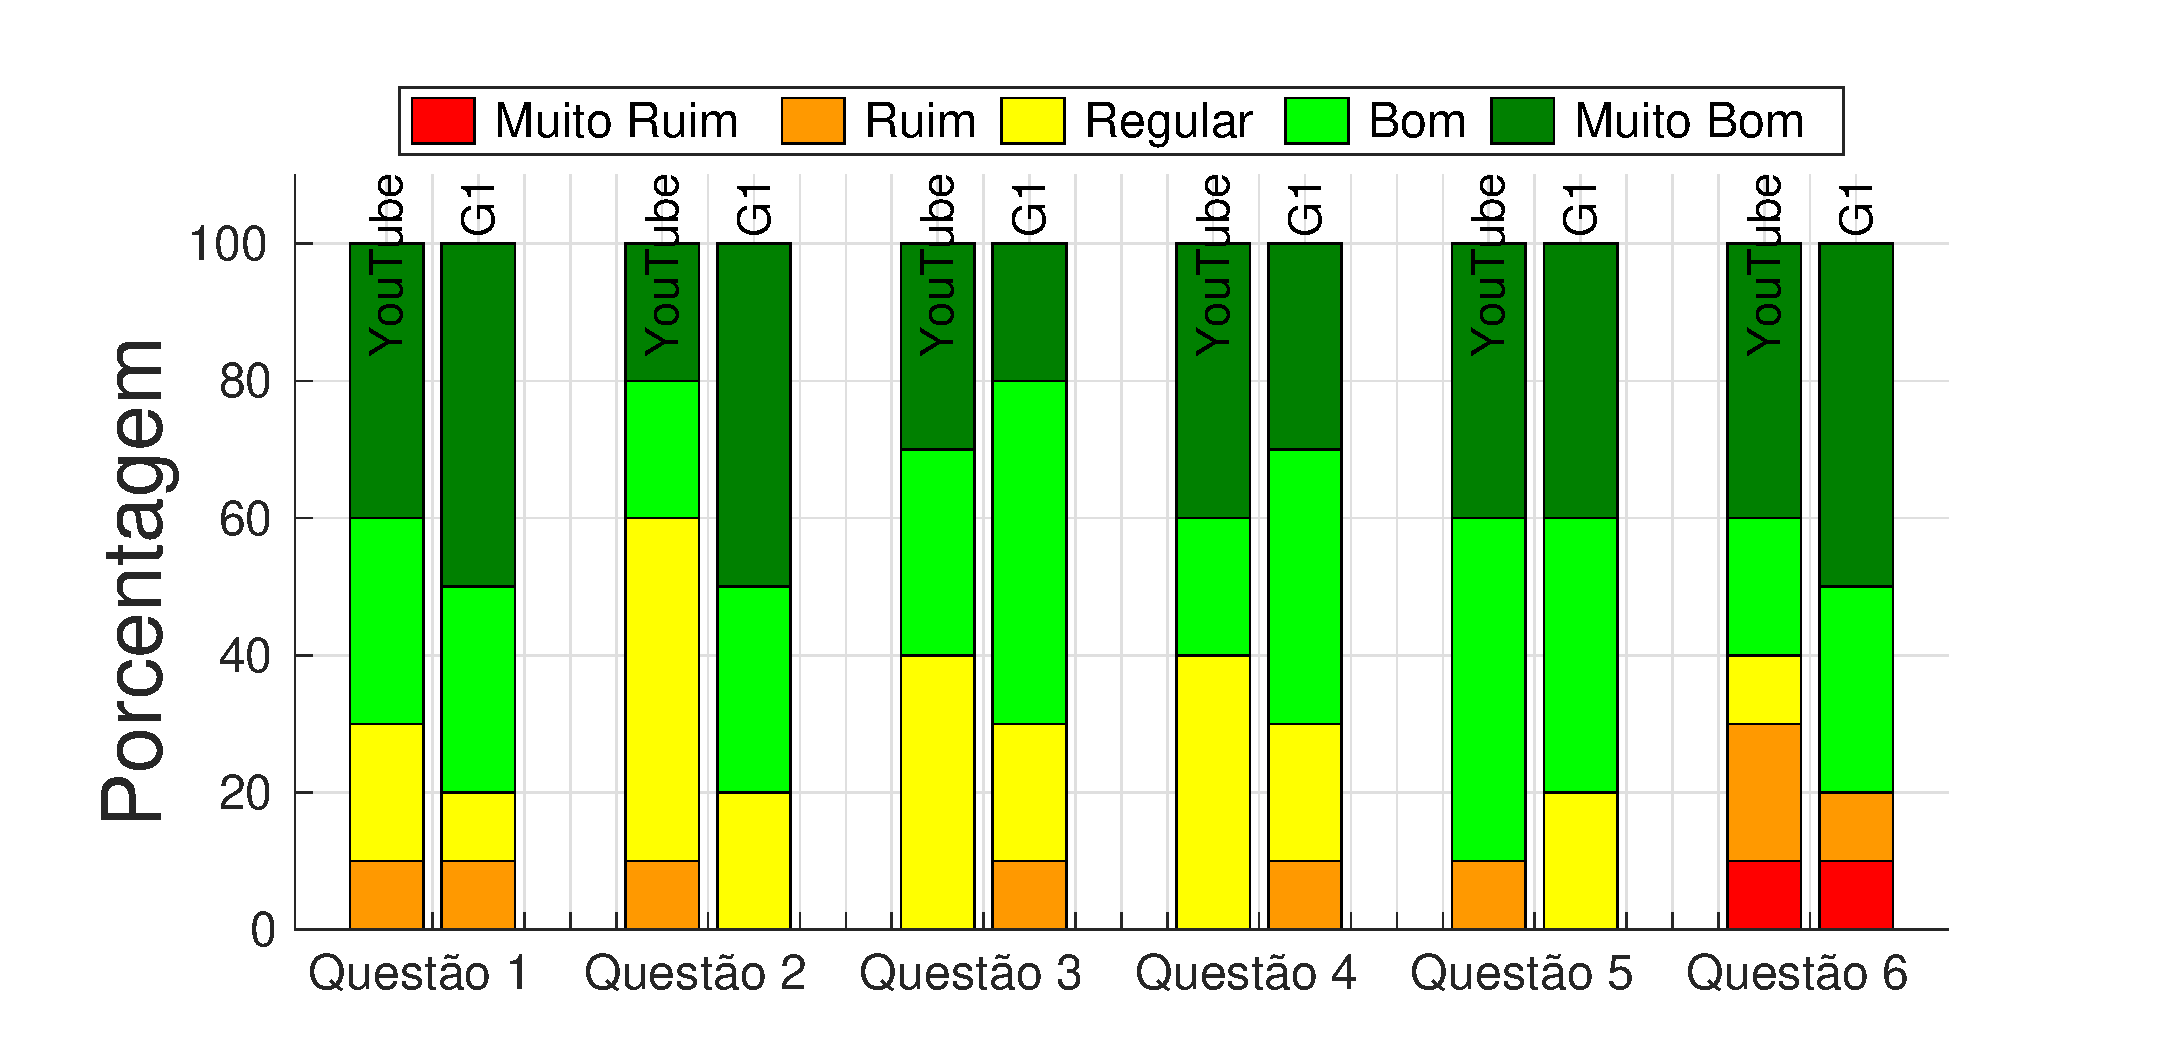
\includegraphics[width=0.9\linewidth]{fig/PuffQuestions}
	\caption{Escala Likert das respostas do protótipo baseado em sopro.}
	\label{fig:PuffQuestions}
	\end{minipage}
\end{figure}



É notório a quantidade superior de respostas que variaram de 1 a 3 para o
\textit{dwell time} em comparação com o clique baseado em sopro. Isso significa
quem a maioria das pessoas não ficaram tão satisfeitas com o desempenho do
\textit{dwell time}. De acordo com os participantes, essa insatisfação ocorreu
principalmente devido a tarefa do G1 ser considerada mais problemática de ser
realizada utilizando o \textit{dwell time}, pois eles precisaram mover o
cursor do \textit{mouse} mais lento que o normal devido a proximidade dos itens
clicáveis localizados no menu do \textit{website}. Diversas vezes, a lentidão do
ponteiro do \textit{mouse} provocou cliques involuntários devido o cursor ficar
sobre uma determinada área por tempo suficiente para a ocorrer a ativação do
clique.

Na questão 1, os usuários relataram que a exeperiência de uso, com o
\textit{dwell time}, foi regular, como pode ser percebido pela maior
concentração de retângulos em amarelo para ambas as tarefas realizadas. Por
outro, com o dispositivo baseado em sopro, a experiência de uso foi considerada
boa, visto que mais de 60\% dos participantes responderam 4 ou 5.  Quanto ao
tempo gasto para realizar uma tarefa, perguntado na questão 2, anlizando apenas
a tarefa do G1, novamente os usuários apontaram que o clique realizado com o
dispositivo baseado em sopro foi melhor, uma vez que apenas 30\% dos
participantes deu uma resposta abaixo de 3, um fato que não ocorreu para o
clique realizado com o \textit{dwell time}.

Os participantes também não ficaram satisfeitos com a precisão do \textit{dwell
time}, já que apenas 20\% dos voluntários deu nota 4 ou 5 para a pergunta 3 na
tarefa do G1. No YouTube, os participantes não tiveram dificuldade em realizar a
tarefa, visto que não era necessário uma grande precisão para executá-la. 

O esforço cognitivo, perguntado na questão 3, foi muito similar para ambos os
métodos de clique. Contudo, analisando a questão 4, onde se perguntava sobre o
esforço físico para realizar as tarefas, é possível notar que na tarefa do
YouTube, o dispositivo baseado em sopro provocou menos esforço físico nos
participantes, pois 90\% das respostas foram 4 ou 5 enquanto que apenas 50\%
das repostas foram 4 ou 5 para o \textit{dwell time}. Por outro lado, na tarefa
do G1, o \textit{dwell time} foi o método que necessitou menos esforço físico
para realizar a tarefa, pois 60\% das respostas foi 5 e outros 30\% das
respostas foi 4. Essa quantidade foi maior que as repostas para o método de
clique baseado em sopro, onde 40\% dos usuários respondeu 5 e outros 40\%
respondeu 4.

A razão pela qual o método de clique baseado em sopro exigiu mais esforço físico
para realizar a tarefa do G1 pode ser a dificuldade que os voluntários tiveram
em realizar a ação de sopro sem movimentar muito a cabeça. Como os itens do menu
do G1 são bastantes próximos uns dos outros, alguns movimentos (incluindo os
executados durante a inspiração e expiração pela boca ao executar a ação de
sopro, que afeta praticamente todo o torso humano), deslocavam o ponteiro do
alvo desejado.

Por fim, é possível observar na última questão que os participantes se sentiram
mais à vontade ao utilizar o dispositivo baseado em sopro, pois a maioria
respondeu 4 ou 5, o que significa que os voluntários se concentraram mais na
realização da tarefa do que no método de clique. Esse fato não se confirmou com o
\textit{dwell time}, pois a maioria das respostas variou de 1 a 3, ou seja, esse
método de clique interferiu na concentração dos participantes na realização das
tarefas. 

\end{subsection}

\begin{subsection}{Discussão Sobre a Questão Subjetiva}

No final dos testes, cada participante foi convidado a responder em um
formulário virtual a seguinte pergunta: ``Com base na sua experiência de uso,
que sugestões você daria para melhoria do dispositivo baseado em sopro?''. Eles 
foram instruídos a se sentir completamente livres para escrever críticas e 
apontar sugestões para a melhoria do dispositivo proposto. Todas as respostas
foram lidas e serão sintetizadas a seguir.

%O maior problema identificado pela maioria dos participantes foi uso do
%\textit{software} eViacam. A falha no rasteamento da face do usuário ao
%posicionar o cursor do \textit{mouse} nos cantos da tela e em ícones pequenos
%frustrou bastante os participantes, que sugeriram a troca do \textit{software}
%de controle do ponteiro do \textit{mouse}.

O dispositivo baseado em sopro proposto neste trabalho foi considerado uma boa
ferramenta para ser utilizada como um método alternativo de clique. Apesar do
bom desempenho do protótipo desenvolvido, houveram alguns problemas encontrados
pelos participantes, principalmente no que diz respeito a cliques involuntários.
Os voluntários sugeriram a substituição do \textit{headset} utilizado como
suporte de sustentação do acionador externo desenvolvido, pois houveram alguns
choques mecânicos causados por essa ferramenta quando os participantes moviam
a cabeça muito rápido.

Houveram também alguns casos onde o participante realizou a ação de sopro e o
clique não ocorreu. Isso aconteceu devido a intensidade do sopro não ser
suficiente para a ativação do clique. Para a maioria dos participantes, a
sensibilidade do dispositivo baseado em sopro estava adequada, pois era
necessário um sopro relativamente fraco para a ativação do clique. No entanto,
alguns voluntários relataram que se sentiriam mais confortáveis se a
sensibilidade fosse aumentada. %Há um potenciômetro acoplado no dispositivo
%proposto que permite o ajuste da sensibilidade, porém apesar de estar ajustado
%em um valor que não necessitava um sopro muito forte nem muito fraco, essa
%sensibilidade gerou desconforto entre alguns usuários. A sugestão dada pelos
%participantes foi a disponibilidade de três níveis de ajuste da sensibilidade
%para que cada usuário possa escolher a intensidade de sopro ideal. 
Eles também enfatizaram que o  dispositivo poderia ter um \textit{feedback}
visual a fim de mostrar para o usuário qual o nível de sensibilidade está
definido no momento.


\end{subsection}

\end{section}

\end{chapter}

\begin{chapter}{Considerações Finais}
Este trabalho apresentou uma proposta de um dispositivo \textit{open-source},
cujo método de entrada é baseado em sopro, que pode ser utilizado como método
alternativo para o controle de eventos de clique de um \textit{mouse}. Para
garantir que o projeto seja d baixo custo, um \textit{software} foi desenvolvido
para comunicar o dispositivo proposto com o computador através da interface de
aúdio. O código fonte e o projeto completo do \textit{hardware} estão
disponíveis ao público no GitHub.

Com base na opinião dos voluntários e no menor numero de erros de cliques
realizados, pode-se concluir que o protótipo desenvolvido neste trabalho é uma
alternativa melhor que o método do \textit{dwell time} para a execução da ação
de clique. Verificou-se que o dispositivo baseado em sopro proposto oferece mais
liberdade para os usuários realizarem tarefas como assistir a um vídeo ou navegar
em um \textit{site} de notícias apesar das limitações impostas pelo
\textit{software} eViacam ao tentar alcaçar os cantos da tela e posicionar o
cursor no alvo correto em itens que se alteram dinâmicamente conforme o ponteiro
passa sobre esses itens, respectivamente.

É importante mencionar que o protótipo desenvolvido foi inspirado por diversos
acionadores externos que têm como sáida o conector de áudio P2 Jack. Esses
dispositivos são tilizados em vários contextos diferentes para ser um
instrumento de interação que geralmente substitui botões ou teclas, que muitas
vezes são uma barreira para as PCD. Portanto o dispositivo projetado neste
trabalho pode ser utilziado como um ferramenta de propósito geral no contexto de
Tecnologia Assistiva para ajudar as PCD realizarem interações de forma
independente com outros dispositivos. Além disso, pode ser uma boa alternativa
aos acionadores externos comerciailizados, pois a maioria desses dispositivos
possuem um alto preço no mercado.

\begin{section}{Trabalhos Futuros}

A ferramenta baseada em sopro desenvolvida neste trabalho foi inicialmente
destinada a ser usada nos sistemas operacionais Windows, Linux e Android. No
entanto, o \textit{software} responsável por captar sinais de áudio e
convertê-los em eventos de cliques foi implementado apenas para plataformas
baseadas em Linux. É necessário desenvolver um software capaz de rodar no
Windows também, provavelmente utilizando a biblioteca de \textit{stream} de
áudio ASIO~\cite{asio} que possui suporte do PortAudio~\cite{portaudio} -- uma
biblioteca \textit{open-source} que permite manipular os sinais da interface de
áudio utilizado a linguagem C++	 Para sistemas Android, por outro lado, a classe
\emph{KeyEvent} tem uma implementação nativa para capturar os cliques do botão
do fone de ouvido através da \textit{flag} de evento
\emph{KEYCODE\_HEADSETHOOK}, fazendo com que o \textit{software} que captura os
dados de áudio não seja mais necessário.

Para evitar os cliques involuntários causados pelo \textit{headset} utilizado
como suporte para o dispositivo baseado em sopro, uma boa alternativa seria
utilizar uma solução semelhante a~\cite{ok}, onde um tubo de PVC fica fixo na
frente do usuário. A outra extremidade do tubo seria colocado em cima do
transdutor piezoelétrico. Dessa forma, choques acidentais com o dispositivo de
sopro seriam evitados, o que resultaria na diminuição dos casos de cliques
involuntários. Contudo, ao utilizar essa solução será necessário substituir o
programa que realiza o controle do cursor do \textit{mouse}. O ideal seria
utilizar um \textit{software} que realiza o controle do ponteiro através dos
movimentos dos olhos, pois o tubo de PCV deverá fixo, impossibilitando o uso de
métodos que utilizem os movimentos da cabeça do usuário como controle do cursor
do \textit{mouse}. Uma segunda alternativa seria construir uma espécie de
capacete qe poderia ser construído utilizando impressoras 3D. Esse capacete
ficaria posicionado na cabeça do usuário, porém essa solução poderia causar
desconforto nos usuários.  

Também é necessário investigar algumas possibilidades de sensores a serem
utilizados como alternativa ao piezo. Como o funcionamento desse transdutor é
causado por estresses mecânicos, qualquer choque mecânico --- a vibração causada
pela movimentação rápida da cabeça, por exemplo --- pode ser suficiente para
ativar o evento de clique. Dispositivos como ~\cite{ok} utilizam  um microfone
de eletreto como sensor para detectar a ação de sopro, então esse sensor pode
ser uma boa solução para substituir o piezo. A desvantagem de usar microfones de
eletreto é que eles são sensíveis a fala, um fato que não se confirma com o
dispositivo proposto neste trabalho que não permite a ativação do clique através
da pressão do ar produzida pela voz humana. Contudo, alguns filtros analógicos
poderiam ser utilizados para garantir a confiabilidade do microfone de eletreto
utilizado como sensor de sopro. 

Outra possibilidade seria usar um sensor de pressão atmosférica (barômetro) para
melhorar a detecção de sopro. O sensor BMP180~\cite{bmp180} é amplamente
utilizado em projetos eletrônicos devido seu baixo custo e facilidade de uso.
Portanto esse sensor poderia ser uma boa alternativa ao piezo.

Seria interessante utilizar o software desenvolvido em conjunto com outros tipos
de interação não convencional, a fim de expandir as possibilidades de interação,
tornando o dispositivo multimodal. Acionadores  que utilizam circuitos
eletromiográficos podem ser usados como um método alternativo de clique, pois
há diversos trabalhos que mostram a eficácia deste tipo de método para tarefas
que demandam um funcinamento de lógica binário. Métodos baseados em aproximação
como o acionador construído em~\cite{Batista17} e até mesmo em dispositivos
que necessitam de contato físico como~\cite{ok} poderiam ser utilizados como
método de interação. Dessa forma, o usuário seria capaz de escolher o melhor
método de interação que se adpta às suas necessidades, o que acabaria ajudando
um maior número de deficiências.

\end{section}

\end{chapter}


%%%%%%%%%%%%%%%%%%%%%%%%%%%%%%%%%%`
%   Referencias bibliograficas   %
%%%%%%%%%%%%%%%%%%%%%%%%%%%%%%%%%%

%\renewcommand\bibname{References}
%\bibliographystyle{../../../public/ABNT-20020112}
%\bibliographystyle{../public/IEEEtran}
%\bibliographystyle{../../../Public/IEEEtran_pt}
\bibliographystyle{IEEEtran}
\bibliography{referencias}

%temorary tag just while there is no \citation
%eliminates no \citation error
\nocite{*}

\clearpage

%%%%%%%%%%%%%%%%%%%%%
%   Appendix        %
%%%%%%%%%%%%%%%%%%%%%
%\appendix

%\input{apendice.tex}
%\input{appendix/append_fpga_flow}
%\input{appendix/append_ad9361_driver}

%%%%%%%%%%%%%%%%%%%%%
%   blank page      %
%%%%%%%%%%%%%%%%%%%%%

\newpage
\thispagestyle{empty}
\mbox{}

%% -- Termino do TCC
\end{document}

